% Document type and layout configurations
\documentclass[pdfa=true]{cacthesis}

% pdf libraries
\usepackage{pdfpages}
\usepackage[a-2b]{pdfx}

% Language configurations
\usepackage[main=english]{babel}
\usepackage[autostyle]{csquotes}

% Literature configurations
\usepackage[
style=alphabetic,
sorting=ynt
]{biblatex}
\addbibresource{bibliography.bib}

% Glossary configurations
\usepackage[acronym,nonumberlist,section=chapter]{glossaries}
\makeglossaries
\newacronym{eudi}{EUDI}{European Digital Identity}
\newacronym{aml}{AML}{Anti-Money Laundering Directive}
\newacronym{mica}{MiCA}{Markets in Crypto-Assets Regulation}
\newacronym{kyc}{KYC}{Know Your Customer}
\newacronym{hd}{HD}{Hierarchical Deterministic}
\newacronym{bip32}{BIP32}{Bitcoin Improvement Proposal 32}
\newacronym{bip39}{BIP39}{Bitcoin Improvement Proposal 39}
\newacronym{bip44}{BIP44}{Bitcoin Improvement Proposal 44}
\newacronym{ppt}{PPT}{probabilistic polynomial-time}
\newacronym{jwt}{JWT}{JSON Web Token}
\newacronym{sdjwt}{SD-JWT}{Selective Disclosure JSON Web Token}
\newacronym{oid4vci}{OID4VCI}{OpenID for Verifiable Credential Issuance}
\newacronym{oid4vp}{OID4VP}{OpenID for Verifiable Presentations}
\newacronym{zkp}{ZKP}{Zero-Knowledge-Proof}
\newacronym{zksnark}{zk-SNARK}{Zero-Knowledge Succinct Non-Interactive Argument of Knowledge}
\newacronym{crs}{CRS}{Common Reference String}
\newacronym{r1cs}{R1CS}{Rank-1 Constraint System}
\newacronym{air}{AIR}{Algebraic Intermediate Representations}
\newacronym{ecdsa}{ECDSA}{Elliptic Curve Digital Signature Algorithm}
\newacronym{oidc}{OIDC}{OpenID Connect}
\newacronym{np}{NP}{nondeterministic polynomial-time}
\newacronym{jws}{JWS}{JSON Web Signature}
\newacronym{fri}{FRI}{Fast Reed–Solomon Interactive Oracle Proof of Proximity}
\newacronym{srs}{SRS}{Structured Reference String}
\newacronym{qap}{QAP}{Quadratic Arithmetic Program}
\newacronym{msm}{MSM}{Multi-Scalar Multiplication}
\newacronym{fft}{FFT}{Fast Fourier Transform}
\newacronym{eddsa}{EdDSA}{Edwards-curve Digital Signature Algorithm}
\newacronym{iop}{IOP}{Interactive Oracle Proof}
\newacronym{ivc}{IVC}{Incrementally Verifiable Computation}

% Diagram configurations
\usepackage{tikz}
\usetikzlibrary{arrows.meta, fit, positioning, shapes.geometric}
\usepackage[edges]{forest}
\usepackage{pgfplots}
\pgfplotsset{compat=1.18}

% Color library
\usepackage{xcolor}

% Table libraries
\usepackage{tabularx}
\usepackage{booktabs}

% List libraries
\usepackage{enumitem}

% Code libraries
\usepackage{listings}
\usepackage{caption}
\usepackage{algorithm}
\usepackage{algpseudocode}

% Listings configurations
\lstset{
	breaklines=true,
	breakatwhitespace=true,
	basicstyle=\ttfamily\small,
	numbers=left,
	numberstyle=\tiny,
	frame=single,
	captionpos=b,
	tabsize=2,
	showstringspaces=false,
	columns=flexible,
}

% Math libraries
\usepackage{amsmath,amssymb}
\usepackage{amsthm}
\newtheorem{definition}{Definition}[chapter]
\usepackage{bm}

% Crypto library
\usepackage{cryptocode}

% Note library
\usepackage{todonotes}

% Link library
\usepackage{hyperref}

\begin{document}
		
	% Activate frontmatter configuration
	\frontmatter
	
	% Define meta-data for \maketitle
	\title{Bridging EUDI Wallets and Web3 via zk-SNARKs}
	\author{Philipp Sommer}
	\date{\today}
	\subject{Master Thesis}
	\publishers{
		\small
		\begin{tabular}{r l}
			Supervisors:	& Prof. Sebastian Faust, Ph.D. \\
							& M.Sc. Philipp-Florens Lehwalder \\
		\end{tabular}
	}
	% Create title page
	\maketitle
	
	% Use declaration file
	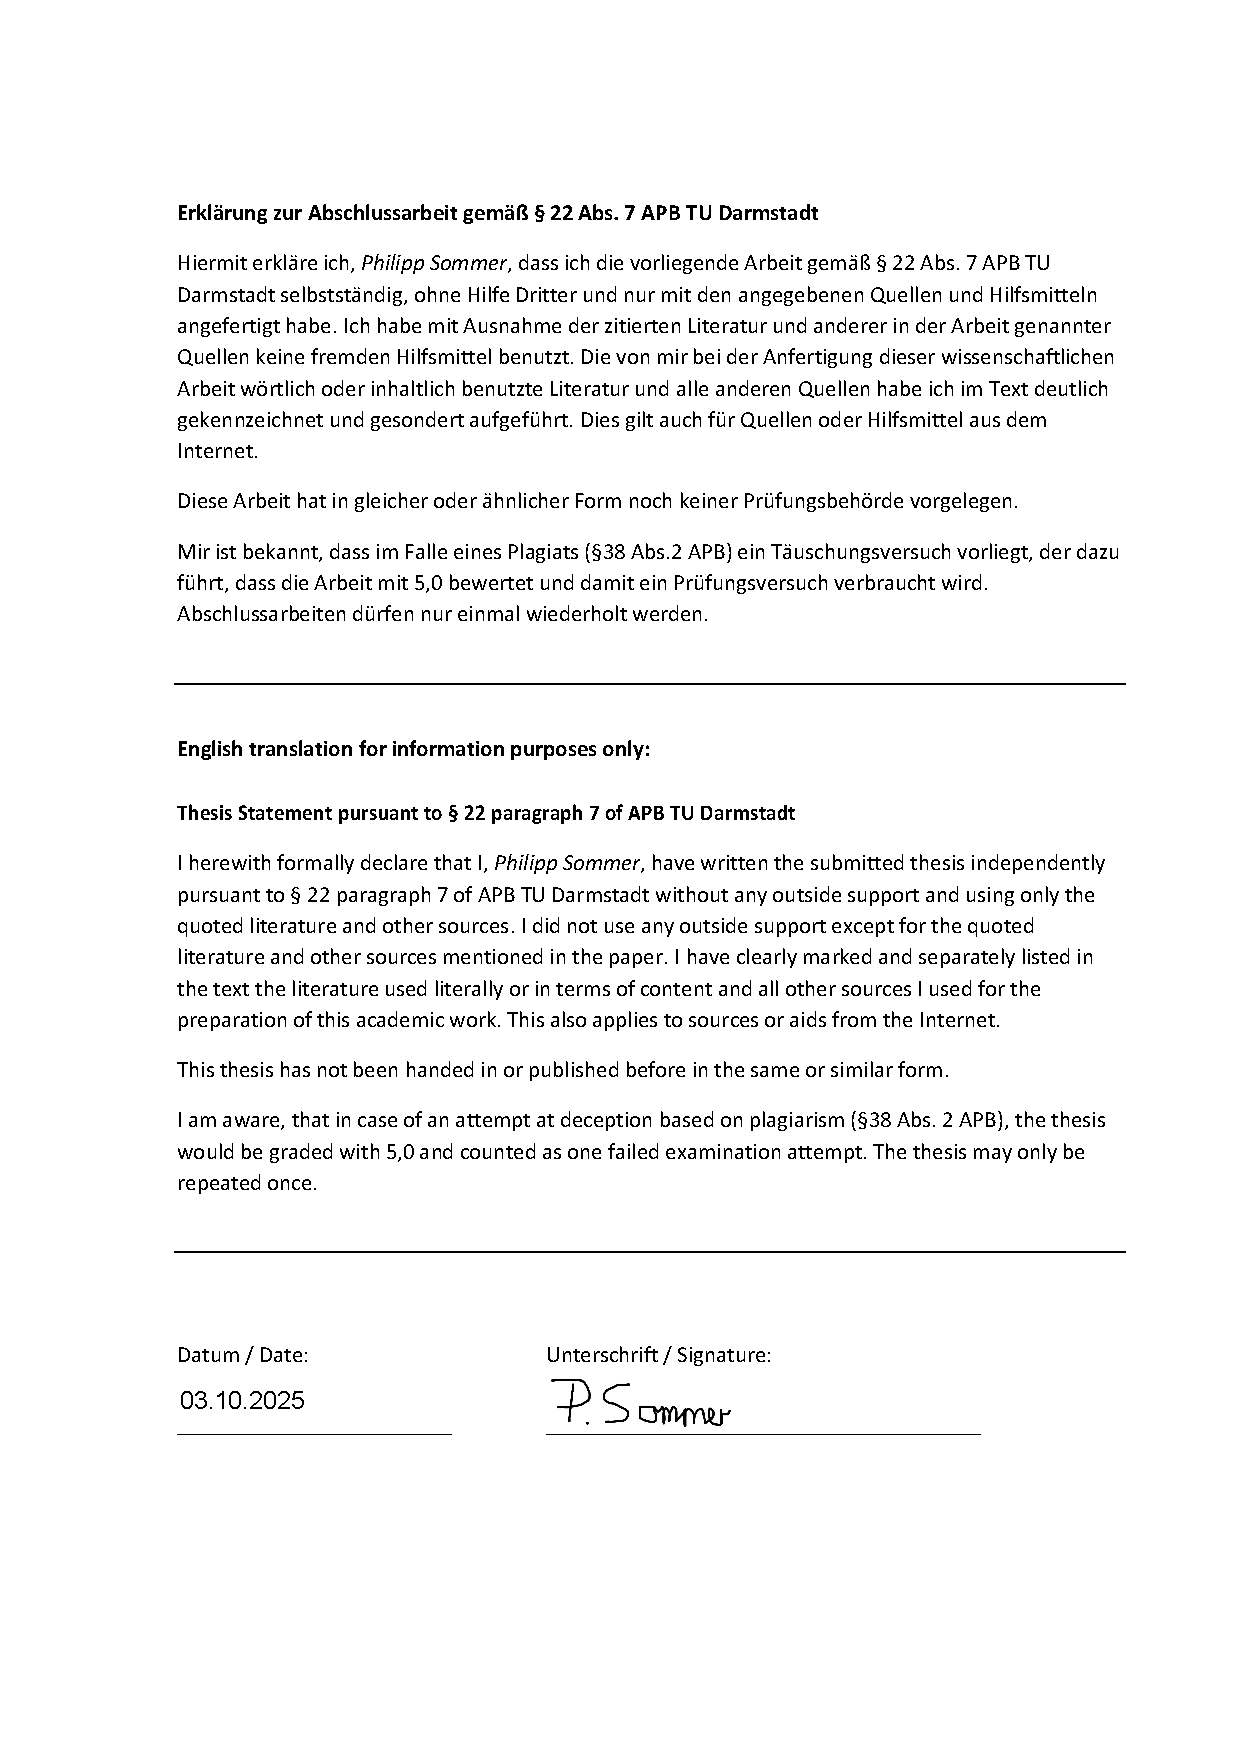
\includepdf{declaration.pdf}
	\section*{Angabe zu eingesetzten KI-Hilfsmitteln / Declaration on the Use of AI Tools}
Im Rahmen dieser Arbeit wurden die folgenden KI-Hilfsmittel verwendet. 
Es wurden ausschließlich Tools eingesetzt, die mit den in den Allgemeinen Prüfungsbestimmungen (APB) vorgegebenen Regeln im Einklang stehen und der guten wissenschaftlichen Praxis entsprechen. Die Angaben dienen der Transparenz hinsichtlich Art, Zweck und Umfang der Verwendung.

\medskip

\noindent
\textit{During the preparation of this thesis, the following AI tools were used. Only tools that comply with the rules of the Allgemeinen Prüfungsbestimmungen (APB) and conform with academic integrity were used. This declaration aims to ensure transparency regarding the type, purpose, and extent of usage.}

\medskip
\vspace{0.5cm}
% \begin{tabularx}{\textwidth}{|X|X|X|}
\begin{tabularx}{\textwidth}{|>{\raggedright\arraybackslash}X|
		>{\raggedright\arraybackslash}X|
		>{\raggedright\arraybackslash}X|}
	\hline
	\textbf{KI-Hilfsmittel / AI Tool} & \textbf{Verwendungszweck / Purpose of Use} & \textbf{Einsatzbereich / Scope of Use} \\
	\hline
	ChatGPT (GPT-4o, GPT-5) & Linguistic support, formulation, and refinement of pre-written content & Editing and improving clarity and style of self-written text. No generation of scientific results or novel content. \\
	\hline
	GitHub Copilot (GPT-4o, GPT-5, Claude Sonnet 4) & Programming assistance, syntax suggestions, and code snippets & Support for implementation details. Used to accelerate coding, not for conceptual design or evaluation. \\
	\hline
	ChatGPT Codex & Problem-solving support when stuck with specific coding issues. Analysis of existing code and suggestion of potential fixes & Used occasionally for debugging and generating repair suggestions when independent solutions were not successful. Final integration and validation done independently. \\
	\hline
\end{tabularx}
\vspace{1cm}

\noindent

	
	\glsdisablehyper
	
	% Force page-break before abstract
	\newpage
	% Use abstract file
	\section*{Abstract}
This thesis investigates how \acrshort{zksnark}s can be applied to bridge EU regulatory requirements, such as identity binding in financial transactions, with the privacy principles of Web3. The central research question is whether monolithic or recursive proof composition offers better efficiency when binding \acrshort{eudi} credentials to blockchain wallets. At its core, the thesis introduces the credential–wallet binding proof ($\pi_{\text{cred-bind}}$), which enables a user to prove possession of a valid \acrshort{eudi} credential together with control of a blockchain wallet public key. This construction is extended with the derived key binding proof ($\pi_{\text{key-bind}}$), which recursively verifies $\pi_{\text{cred-bind}}$ and establishes the binding for child public keys. Both proofs are designed to satisfy the standard \acrshort{zksnark} properties of completeness, knowledge soundness, and zero-knowledge.

We implement $\pi_{\text{cred-bind}}$ as a monolithic Groth16 proof using Circom, snarkjs, and RapidSnark, and also as a monolithic Plonky2 proof, while $\pi_{\text{key-bind}}$ is realized as a recursive Plonky2 proof. All implementations incorporate targeted optimizations to improve proving efficiency while preserving correctness and security. Our evaluation shows that the Groth16 instantiation achieves the highest efficiency, with proof generation in 8.24 seconds, a proof size of 803 bytes, and verification in 0.01 seconds, outperforming both Plonky2 variants. Within Plonky2, recursion yields clear efficiency gains over its monolithic baseline, reducing proving time from 85.05 to 18.39 seconds and proof size from 179.6 to 163 kB.

A simplified cost model explains these results: Groth16 benefits from small constant factors and constant-size proofs, while Plonky2 incurs higher costs due to domain padding and the overhead of FFTs, Merkle commitments, and FRI queries. Nova was also considered as a folding-based alternative, but full integration was not possible because gadget support for the required curves is still missing.

The results highlight three main contributions of this work. First, the definition of two new \acrshort{zksnark}-based proofs for linking \acrshort{eudi} credentials with blockchain wallets. Second, the implementation of both monolithic and recursive approaches in Groth16 and Plonky2. Third, an empirical evaluation and cost model to clarify the performance trade-offs. Taken together, these findings demonstrate that \acrshort{zksnark}s provide a viable cryptographic bridge between EU-compliant digital identity and decentralized wallets. They show that Groth16 currently offers the most efficient solution, while recursion within Plonky2 improves performance internally but remains less competitive across systems. This establishes both the feasibility and the limitations of privacy-preserving yet regulation-compliant identity integration in Web3.
	% Force page-break after abstract
	\newpage
	
	% Create table of contents, figures, tables
	\tableofcontents
	\cleardoublepage
	\phantomsection
	\addcontentsline{toc}{chapter}{List of Abbreviations}
	\printglossary[type=\acronymtype, title=List of Abbreviations, toctitle=List of Abbreviations]
	\listoffigures
	\listoftables
	
	% Activate mainmatter configuration
	\mainmatter
	
	% Use chapter files
	\chapter{Introduction}
\label{chap:introduction}

\section{Motivation and problem statement}
\label{sec:motivation-problem-statement}
% EU context
In recent years, the concept of digital identity has become a central element of the digital transformation in the European Union (EU). To address the fragmentation of national solutions and to ensure secure, interoperable, and privacy-preserving identity management, the EU launched the \textit{\acrfull{eudi}} initiative~\cite{EUCommission2021, EURegulation2024}. At its core is the \textit{\acrshort{eudi} Wallet}, a user-controlled application for storing and presenting legally verified credentials such as identification data, certificates, and electronic signatures. Under Regulation (EU 2024/1183), each Member State must provide a compliant wallet. The \acrshort{eudi} Wallet serves as a cryptographic anchor for legally verified credentials and enables user-controlled identity management across borders and sectors. However, the \acrshort{eudi} framework is closely tied to broader EU regulation, including the \textit{\acrfull{aml}} and the \textit{\acrfull{mica}}~\cite{EUDirective2015AML,EURegulation2023MiCA}. These measures require that users in financial services and regulated value transfers can be linked to verifiable legal identities, typically through \textit{\acrfull{kyc}} procedures and digitally signed credentials. Together, they position the \acrshort{eudi} Wallet as a central element of the EU's digital identity ecosystem. Through trusted credentials and selective disclosure, the wallet provides a standardized basis for privacy-preserving digital identity management across the EU.

% Web3 context
In contrast to this regulatory vision, Web3 represents a fundamentally different paradigm for identity and interaction. It promotes decentralization, user autonomy, pseudonymity, and self-sovereign identity systems \cite{bambacht2022web3}. These principles are reflected in blockchain-based architectures, which deliberately avoid inherent links to users’ real-world identities. A common technical component in such systems is the use of \acrfull{hd} wallets, most notably specified in \acrfull{bip32} \cite{bip32, Das2019, narayanan2016bitcoin}. HD wallets derive child keys from a parent key, which prevents key reuse and preserves unlinkability across multiple interactions, while never embedding legal identity information. This architecture supports privacy and censorship resistance, allowing pseudonymous interaction without relying on trusted intermediaries. At the same time, it conflicts with EU regulatory frameworks that require strong identity binding in financial and legally accountable applications. Directly linking an \acrshort{eudi} credential to a wallet key would break unlinkability, undermining Web3’s privacy guarantees. Moreover, prior work shows that key compromise in \acrshort{hd} wallets can propagate along the hierarchy, potentially exposing large parts of a user’s assets~\cite{Das2019}. Thus, weakening unlinkability not only threatens privacy but also creates concrete security risks such as large-scale key exposure and asset loss.

% Problem statement
Bridging the gap between the requirements of regulatory identity verification and the privacy-preserving design principles of decentralized architectures presents a fundamental design challenge at the intersection of these two paradigms. This challenge arises on two levels. First, users must be able to prove that they possess a valid \acrshort{eudi} credential and control a specific blockchain wallet typically represented by a public key, without revealing any link between their legal identity and the wallet. Second, users must demonstrate that a child key used in a transaction has been correctly derived from a parent key of the wallet, without compromising the unlinkability between individual transactions. In both cases, the goal is to preserve privacy while enabling compliance, without disclosing identifying attributes or wallet internals. This conflict between regulatory identity binding and cryptographic unlinkability can be addressed using a \acrfull{zkp}, which is a group of cryptographic protocols that allows one party (the prover) to convince another party (the verifier) that a statement is true, without revealing any information beyond the validity of the statement itself \cite{narayanan2016bitcoin, 10.1145/22145.22178}. A particularly promising type of \acrshort{zkp}s is the \acrfull{zksnark}. The term refers to proof systems which enable short, non-interactive, and efficiently verifiable proofs for general statements expressed over arithmetic circuits \cite{liang2025}. Importantly, they offer strong privacy guarantees, making them ideal for regulatory-compliant yet privacy-preserving blockchain use cases \cite{rosenberg2023, Baldimtsi_2024}. At a methodological level, \acrshort{zksnark}s can be realized either by encoding all required constraints in a single circuit, or by composing multiple proofs in a recursive manner. Which of these two composition strategies yields better efficiency in the specific context of binding EU-compliant credentials to blockchain wallets constitutes the central question of this thesis.

\section{Contribution and structure}
\label{sec:contribution-structure}
This thesis addresses the challenge of bridging the gap between regulatory identity compliance and privacy-preserving identity management in decentralized systems. The main contribution consists of the design and implementation of zero-knowledge circuits for the following statements:

The first is the \emph{credential–wallet binding}, which enables a user to prove possession of a valid \acrshort{eudi} credential while demonstrating control over a blockchain wallet represented by a public key. Both the credential and the wallet’s secret key remain private witness inputs to the \acrshort{zksnark}, ensuring that no direct link between them is revealed. The second is the \emph{derived key binding}, which proves that a child public key used in a transaction has been correctly derived from a parent public key of the wallet. Here, the child key is public, whereas the parent key remains part of the private witness, thus preserving unlinkability between individual transactions.

\medskip
The two statements are implemented using distinct composition approaches. The credential–wallet binding proof is realized as a monolithic circuit that encapsulates all required constraints in a single proof. The derived key binding proof, in contrast, follows a recursive composition, in which the circuit not only enforces correct key derivation but also verifies a previously generated credential–wallet binding proof. This separation supports flexible deployment and enables a structured evaluation of performance trade-offs between the two approaches.
\begin{quote}
	\textbf{Research question:} 
	\textit{Which composition approach, monolithic or recursive, offers better efficiency in terms of proof size, generation time, and verification performance when binding EU-compliant credentials to blockchain wallet operations using \acrshort{zksnark}s?}
\end{quote}
To address this question, the thesis implements and optimizes both approaches and compares their practical performance to assess their suitability for real-world applications. The structure of the thesis is as follows. Chapter~\ref{chap:preliminaries} introduces the foundational concepts and technologies used throughout this work, including wallets, hierarchical key derivation schemes, and \acrshort{zksnark}s. Chapter~\ref{chap:construction} defines the system model with roles, assumptions, and requirements, and then presents the construction of the \acrshort{zksnark}-based proof systems. Chapter~\ref{chap:implementation-evaluation} describes the realization of both proofs using monolithic and recursive composition, together with selected design decisions and implementation-specific optimizations. It further reports the empirical evaluation of proof size, generation time, and verification time, and discusses the implications of the results for real-world deployments. Finally, Chapter~\ref{chap:conclusion} summarizes the findings of the thesis and outlines directions for future work.

\section{Related work}
\label{sec:related-work}
Recent advances in \acrshort{zkp}s have sparked interest in applying \acrshort{zksnark}s to identity-related use cases in decentralized environments. Prominent examples include \textit{zkLogin} and \textit{zkCreds}, which demonstrate how existing identity credentials can be combined with \acrshort{zksnark}s to enable privacy-preserving authentication and credential systems~\cite{Baldimtsi_2024,rosenberg2023}. \textit{zkLogin} leverages \acrfull{oidc} tokens from traditional identity providers to enable pseudonymous login to blockchain applications using \acrshort{zksnark}s. The authors identify latency as a major challenge in mobile scenarios and propose hybrid delegation schemes and proof caching to reduce user-perceived delay. In contrast, \textit{zkCreds} constructs anonymous credentials from existing identity documents using general-purpose \acrshort{zksnark}s, proving in zero knowledge that a committed credential matches signed legacy data (e.g., e-passport), with issuance recorded via a Merkle-based bulletin board. Their system faces efficiency bottlenecks due to the complexity of verifying Merkle tree inclusion proofs and advanced circuit features such as linkable show proofs and clone resistance, which increase proving costs. Beyond such blockchain-oriented systems, other work has focused on credential schemes with a stronger emphasis on selective disclosure and compatibility with existing infrastructures. Frigo and Shelat propose an anonymous credential scheme leveraging the \acrfull{ecdsa}, and highlight that widely used curves such as \textit{secp256r1} are not optimized for \acrshort{zksnark} circuits due to their non-native arithmetic. Instead of relying on ad-hoc gadgets, they construct a dedicated sum-check and Ligero-based proof system tailored for \textit{secp256r1}, and demonstrate that verification can be performed within tens of milliseconds even on mobile devices~\cite{cryptoeprint:2024/2010}. Paquin et al. introduce \textit{Crescent}, an anonymous credential system that enables selective disclosure of existing credentials such as mobile driver’s licenses. Their construction relies on \acrshort{zksnark}-based verification of \acrshort{ecdsa}-signed credentials, thereby providing privacy guarantees such as unlinkability without requiring the involvement of new issuing authorities or fundamental changes to existing credential infrastructures~\cite{cryptoeprint:2024/2013}. Other initiatives such as \textit{zkKYC} and Sun et al. investigate zero-knowledge-based approaches for \acrshort{kyc} compliance in decentralized finance (DeFi) and general public blockchain environments~\cite{cryptoeprint:2022/321,su142114584}. Rathee et al. identify the cost of on-chain credential verification with \acrshort{zksnark}s as a major scalability constraint and propose batching strategies and audit-token reuse to reduce per-user overhead~\cite{cryptoeprint:2022/1286}. Furthermore, Biedermann et al. present a systematization of efforts to connect \acrshort{eudi} infrastructure with decentralized Web3 technologies~\cite{Biedermann_2024}. Their work outlines conceptual and technical challenges but remains theoretical and does not provide a concrete implementation. Buterin et al. emphasize the need for privacy-preserving compliance mechanisms in blockchain systems and highlight the role of \acrshort{zkp}s as a central tool in achieving this balance~\cite{BUTERIN2024100176}.

While prior approaches demonstrate the potential of \acrshort{zkp}s for privacy-preserving identity verification, they remain limited in scope. Blockchain-oriented systems such as \textit{zkLogin}, \textit{zkCreds}, or \textit{zkKYC} do not address EU-compliant credentials, whereas credential-focused work such as \textit{Crescent} or the scheme by Frigo and Shelat does not provide a concrete mechanism to bind \acrshort{eudi} credentials to blockchain wallets. In particular, no available implementation guarantees unlinkability both between a user’s credential and the parent key of a blockchain wallet and among the child keys derived from that parent key.

This thesis addresses this gap by designing a \acrshort{zksnark}-based proof system that combines credential–wallet binding with derived key binding. The system enables a user to prove possession of a valid \acrshort{eudi} credential and control over a blockchain wallet, without revealing either element or creating a direct link between them. It further allows the user to prove that a child key was correctly derived from a parent key of the wallet while maintaining unlinkability. By implementing the system both as a monolithic circuit and in a recursive composition, the thesis examines whether recursion yields efficiency gains in proof size, generation time, and verification performance.

	\chapter{Preliminaries}
\label{chap:preliminaries}
This chapter introduces the conceptual and technical foundations necessary to understand the design and implementation of the proposed solution for privacy-preserving identity binding. It provides an overview of digital wallets and key derivation mechanisms used in decentralized systems, outlines the structure and objectives of the \acrshort{eudi} Wallet, and explains \acrshort{zksnark}s used in this work.

\section{Cryptographic wallets}
\label{sec:blockchain-wallets}
\providecommand{\WalletOverviewFigure}{
	\begin{figure}[htbp]
		\centering
		\begin{tikzpicture}[
			node distance=1.2cm and 1.6cm,
			every node/.style={font=\footnotesize\ttfamily},
			align=center,
			box/.style={draw, minimum width=4.2cm, minimum height=3.6cm}
			]
			
			\node[box] (wallet1) {
				Wallet 1\\[0.3cm]
				Secret key:\\
				0245a349...6130\\[0.3cm]
				Public key:\\
				0357048e...ce2b
			};
			
			\node[box, right=of wallet1] (wallet2) {
				Wallet 2\\[0.3cm]
				Secret key:\\
				df60ed2d...f9bb\\[0.3cm]
				Public key X:\\
				d50cf8d1...ed45\\[0.3cm]
				Public key Y:\\
				71bf8c8b...e08e
			};
			
			\node[box, right=of wallet2] (wallet3) {
				Wallet 3\\[0.3cm]
				Secret key:\\
				8c10c0c2...42e6\\[0.3cm]
				Public key:\\
				037f9449...a3abc
			};
			
			\node[below=2.6cm of wallet1] (addr1) {\shortstack{Address (BTC)\\16tay2XDBFSV3tBpTNfHCyRAt\\WarT1hWdE}};
			\node[below=2.6cm of wallet2] (addr2) {\shortstack{Address (ETH)\\0x35a53747aba81a63\\579b6c534d16db98\\1d677889}};
			\node[below=2.6cm of wallet3] (addr3) {\shortstack{Address (BTC)\\18kh6FQB7QwC9NBynN7pNWhe\\b6CmsDNSdR}};
			
			\draw[->] (wallet1.south) -- node[right, yshift=-4pt] {\scriptsize Derivation} (addr1.north);
			\draw[->] (wallet2.south) -- node[right, yshift=-4pt] {\scriptsize Derivation} (addr2.north);
			\draw[->] (wallet3.south) -- node[right, yshift=-4pt] {\scriptsize Derivation} (addr3.north);
			
			\node[fit=(wallet1)(wallet2), draw, dashed, label=above:{Account 1}, inner sep=0.5cm, minimum height=5.1cm] (acc1) {};
			\node[fit=(wallet3), draw, dashed, label=above:{Account 2}, inner sep=0.5cm, minimum height=5.1cm] (acc2) {};
			
			\node[fit=(acc1)(acc2), draw, dashed, label=above:{Example identity}, inner sep=0.5cm] (identity) {};
			
		\end{tikzpicture}
		\caption{Relationship between identity, accounts, wallets, key pairs, and blockchain addresses.}
		\label{fig:wallet-overview}
	\end{figure}
}

\providecommand{\BIPWalletFigure}{
	\begin{figure}[htbp]
		\centering
		\begin{tikzpicture}[
			level 1/.style={sibling distance=4cm},
			level 2/.style={sibling distance=2cm},
			level 3/.style={sibling distance=2cm},
			every node/.style={circle, draw, minimum size=1cm, align=center, font=\small},
			selected/.style={fill=gray!30},
			dashed edge/.style={draw, thick, dashed},
			solid edge/.style={draw, thick}
			]
			
			\node[selected]{m}
			child[solid edge] {node[selected] {$0'$}
				child[dashed edge] {node {0}}
				child[solid edge] {node[selected] {1}
					child[dashed edge] {node {0}}
					child[dashed edge] {node {1}}
					child[solid edge] {node[selected] {$2'$}}
				}
				child[dashed edge] {node {2}}
			}
			child[dashed edge] {node {1}}
			child[dashed edge] {node {2}};
			
		\end{tikzpicture}
		\caption{Derivation path $m/0'/1/2'$ in a BIP32 hierarchical tree.}
		\label{fig:bip32-path}
	\end{figure}
}

\providecommand{\StatefulWalletFigure}{	
	\begin{figure}[htbp]
		\centering
		\begin{tikzpicture}[
			every node/.style={font=\sffamily\small},
			box/.style={draw, fill=gray!20, rounded corners, minimum width=1.4cm, minimum height=0.9cm, align=center},
			proc/.style={draw, rounded corners, minimum width=1.6cm, minimum height=0.9cm},
			arrow/.style={-Stealth, thick},
			]
			
			\node[proc] (keygen) at (0,0) {\texttt{KeyGen}};
			
			\node[box] (pk0) at (2.2,1.8) {pk\textsubscript{0}};
			\node[box] (sk0) at (2.2,-1.8) {sk\textsubscript{0}};
			\node[box] (st) at ($(pk0)!0.5!(sk0)$) {$st$}; % <-- Neu positioniert in der Mitte
			
			\node[box] (id) at (4.5,0) {$i$};
			
			\node[proc] (pkder) at (4.5,1.8) {\texttt{PKDer}};
			\node[proc] (skder) at (4.5,-1.8) {\texttt{SKDer}};
			
			\node[box] (pki) at (6.7,1.8) {pk\textsubscript{i}};
			\node[box] (ski) at (6.7,-1.8) {sk\textsubscript{i}};
			
			\draw[arrow] (keygen) -- (st);
			\draw[arrow] (st) -- (pk0);
			\draw[arrow] (st) -- (sk0);
			
			\draw[arrow] (pk0) -- (pkder);
			\draw[arrow] (st) -- (pkder);
			\draw[arrow] (id) -- (pkder);
			\draw[arrow] (pkder) -- (pki);
			
			\draw[arrow] (sk0) -- (skder);
			\draw[arrow] (st) -- (skder);
			\draw[arrow] (id) -- (skder);
			\draw[arrow] (skder) -- (ski);
			
		\end{tikzpicture}
		\caption{Session key derivation in a stateful wallet}
		\label{fig:stateful-wallet}
	\end{figure}
}


\paragraph{Definition and purpose}
A cryptographic wallet is a data structure that manages pairs of secret and public keys. These keys are used to authorize blockchain transactions and to demonstrate control over specific addresses. Ownership of assets is not determined by the wallet itself but by the ability to generate valid digital signatures with the corresponding secret key. In most blockchain protocols, addresses are derived from public keys via cryptographic hash functions (e.g., RIPEMD-160 in Bitcoin or Keccak-256 in Ethereum)~\cite{buterin2014ethereum}. Public keys therefore constitute the cryptographic basis from which blockchain-specific addresses are generated. Since this work does not rely on address semantics, wallets are represented directly by their public keys, independent of protocol-specific address formats. Beyond transaction authorization, recent work has highlighted the emerging role of wallets as cryptographic anchors in decentralized identity systems, where they enable secure key derivation and verifiable user control~\cite{Das2019,Das2021}.


\paragraph{Wallet types}
From a key management perspective, wallets can be classified into non-deterministic, deterministic, and hierarchical deterministic (HD) designs \cite{antonopoulos2023}. Non-deterministic wallets generate each key independently using fresh randomness, offering high entropy and forward secrecy, but suffering from backup complexity and lack of structure \cite{narayanan2016bitcoin}. Deterministic wallets resolve this by using a fixed root secret (the master seed) from which all subsequent key pairs are derived using deterministic key derivation functions \cite{Das2019}. HD wallets, a subclass of deterministic wallets, extend this idea by introducing a tree structure that enables organized derivation of keys for different applications, accounts, or assets \cite{bip32, bip44}. This model supports structured backups, flexible key derivation, and organized key separation across applications or accounts \cite{antonopoulos2023}.

\paragraph{\acrshort{hd} wallets}
The \acrshort{hd} wallet standard is specified across the three key Bitcoin Improvement Proposals \acrshort{bip32}, \acrshort{bip39}, and \acrshort{bip44}~\cite{bip32,bip39,bip44}. In addition, \acrshort{hd} wallets are widely used in modern decentralized systems and are implemented in software, hardware, and browser-based environments. The core functionality of these wallets is formalized below. Although there is no formal cryptographic definition of \acrshort{hd} wallets in the literature, the following description summarizes their core functions as implemented in \acrshort{bip32}-based schemes.

\begin{definition}[\acrshort{hd} Wallet]
	A \textit{\acrshort{hd} wallet} is a deterministic key management scheme specified by the following algorithms:
	
	\begin{itemize}
		\item $(pk_0, sk_0, cc_0) \leftarrow \texttt{KeyGen}(s)$: A \acrfull{ppt} algorithm that takes as input a uniformly random seed $s$ and outputs a master secret key $sk_0$, a corresponding public key $pk_0$, and a chain code $cc_0$.
		
		\item $(sk_i \text{ or } pk_i, cc_i) \leftarrow \texttt{KeyDer}(sk_p, pk_p, cc_p, i)$: A deterministic algorithm that takes as input a parent key pair $(sk_p, pk_p)$, a chain code $cc_p$, and an index $i$, and outputs a child key $sk_i$ or $pk_i$ and a new chain code $cc_i$.\footnote{The \texttt{KeyDer} function abstracts over both hardened and non-hardened derivations as defined in the \acrshort{bip32} specification. The exact derivation logic is shown in Table~\ref{tab:hd-derivation}.}
		
		\item $\sigma \leftarrow \texttt{Sign}(sk, m)$: A deterministic signing algorithm that takes as input a secret key $sk$ and a message $m$, and outputs a digital signature $\sigma$ over $m$.
		
		\item $b \leftarrow \texttt{Verify}(pk, m, \sigma)$: A deterministic verification algorithm that takes as input a public key $pk$, a message $m$, and a signature $\sigma$, and outputs a bit $b \in \{0,1\}$, where $b = 1$ if $\sigma$ is a valid signature on $m$ under $pk$, and $b = 0$ otherwise.
	\end{itemize}
\end{definition}

These functions form the foundation for secure key management, identity binding, and transaction authorization in blockchain applications. Furthermore, \acrshort{bip32} defines how keys and associated chain codes are recursively derived in a tree structure. Each node can produce child keys either through non-hardened or hardened derivation paths. Non-hardened derivations allow public key delegation, where child public keys can be derived from a parent public key and chain code. Hardened derivations require the parent secret key and prevent certain compromise scenarios like recovering a parent secret key from a child secret key and the parent public key. The derivation process begins with a root seed, which is converted into a master key and chain code as defined above by the \texttt{KeyGen} algorithm. Subsequent child keys are derived recursively using the algorithms specified in table~\ref{tab:hd-derivation}.

\begin{table}[htbp]
	\centering
	\begin{tabular}{c|c}
		\toprule
		\textbf{Non-hardened derivation} & \textbf{Hardened derivation} \\
		\midrule
		Secret key derivation: & Secret key derivation: \\
		$(sk_i, cc_i) \leftarrow \texttt{KeyDer}(sk_p, cc_p, i)$ & $(sk_i, cc_i) \leftarrow \texttt{KeyDer}(sk_p, cc_p, i')$ \\
		Public key derivation: & Public key derivation: \\
		$(pk_i, cc_i) \leftarrow \texttt{KeyDer}(pk_p, cc_p, i)$ & $pk_i \leftarrow \texttt{KeyDer}(sk_i)$ \\
		\bottomrule
	\end{tabular}
	\caption{Comparison of \acrshort{bip32} derivation types.}
	\label{tab:hd-derivation}
\end{table}

In most blockchain applications, \acrshort{hd} wallets are instantiated over elliptic-curve key pairs based on \acrshort{ecdsa} with the curve \emph{secp256k1}. This curve is specified by the Standards for Efficient Cryptography Group (SECG) and widely used in Bitcoin and Ethereum~\cite{SEC2}. It is also listed among the cryptographic algorithms approved for use in the EU context~\cite{SOGIS-ACM-1.3}.

Each key in the \acrshort{hd} wallet hierarchy is identified using a path notation of the form \texttt{m/level1/level2/.}. Hardened derivations are denoted by an apostrophe, e.g., \texttt{m/44'/0'/0'/0/0}. \acrshort{bip39} introduces mnemonic phrases as a human-readable representation of the master seed, improving usability and security. \acrshort{bip44} further formalizes the derivation path into five semantic levels: \texttt{m / purpose' / coin\_type' / account' / change / address\_index}. This allows wallet applications to organize keys for different cryptocurrencies, user accounts, and address purposes in a standardized and interoperable way. For the purposes of this thesis, we abstract from the full \acrshort{bip44} hierarchy and adopt a flat derivation model. Concretely, the designated parent key $pk_0$ is placed at the account level (\texttt{m/44'/0'/0'}), and child keys $pk_i$ are derived in a single non-hardened step as \texttt{m/44'/0'/0'/i}, thereby omitting the intermediate \texttt{change} and \texttt{address\_index} levels. Figure~\ref{fig:bip32-path} illustrates a derivation path within the \acrshort{bip32} hierarchical tree.

\BIPWalletFigure

\paragraph{Stateful wallets}
This type of wallet extends deterministic key derivation by introducing an internal state that evolves over time. \acrshort{hd} wallets as defined in \acrshort{bip32}~\cite{bip32} are stateless. Every key can be recomputed solely from the seed and index, and no information about past derivations is stored. In contrast, stateful wallets maintain an additional parameter \emph{st} that is updated on each derivation, for example by incrementing a counter or recording previously used indices. This evolving state enables advanced key management patterns such as controlled key rotation, one-time keys, or unlinkable session identifiers. Even if the same index is reused, the derivation yields different results, supporting properties like forward secrecy and prevention of address reuse. Structurally, stateful wallets still rely on a seed-based hierarchy but deviate from the fixed tree structure of \acrshort{hd} wallets. As a result, some interoperability guarantees of \acrshort{bip32}-compliant designs are lost, while more dynamic and context-sensitive key derivation strategies become possible, which are particularly relevant in identity-oriented systems~\cite{Das2021,erinle2025sokdesignvulnerabilitiessecurity}.

\section{EUDI Wallet}
\label{sec:eudi-wallet}
\providecommand{\EudiFigure}{	
	\begin{figure}[h!]
		\centering
		\begin{tikzpicture}[
			font=\sffamily\small,
			node distance=0.7cm,
			box/.style={draw, rounded corners, fill=gray!10, minimum width=6cm, minimum height=1.4cm, align=left},
			centerlabel/.style={font=\bfseries\large, align=center},
			arr/.style={-Stealth, thick}
			]
			
			\node[centerlabel] at (0,6.6) {EUDI Wallet Architecture};
			
			\node[centerlabel] at (0,5.8) {Protocol layer};
			\node[box] (oid4vci) at (-3,4.8) {\textbf{OID4VCI} \\ Receive credentials from issuer};
			\node[box] (oid4vp) at (3,4.8) {\textbf{OID4VP} \\ Present credentials to verifier};
			
			\node[centerlabel] at (0,3.6) {Credential layer};
			\node[box] (cred1) at (-3,2.6) {\textbf{Verifiable Credential 1}\\ Claims: name, birthdate};
			\node[box] (cred2) at (3,2.6) {\textbf{Verifiable Credential 2}\\ Claims: nationality};
			
			\node[centerlabel] at (0,1.4) {Crypto layer};
			\node[box] (crypto1) at (-3,0.4) {\textbf{Key Pair 1}\\ $sk_1$, $pk_1$ \\ Bound to cred1 ($pk_1$ in cnf)};
			\node[box] (crypto2) at (3,0.4) {\textbf{Key Pair 2}\\ $sk_2$, $pk_2$ \\ Bound to cred2 ($pk_2$ in cnf)};
			
			\draw[arr] (oid4vci) -- (cred1);
			\draw[arr] (oid4vp) -- (cred2);
			
			\draw[arr] (cred1) -- (crypto1);
			\draw[arr] (cred2) -- (crypto2);
			
		\end{tikzpicture}
		\caption{Modular components of the EUDI Wallet reference implementation.}
		\label{fig:eudi-wallet}
	\end{figure}
}


\paragraph{Overview}
The reference implementation of the \acrshort{eudi} Wallet, maintained by the European Commission as an open-source project\footnote{\url{https://github.com/eu-digital-identity-wallet}},
is organized into modular components that separately handle cryptographic key management, credential storage, and protocol interactions. The following description summarizes only the technical aspects that are directly relevant to the construction presented in this thesis. 

The architecture follows a layered model comprising three components. The \emph{crypto layer} manages elliptic curve key pairs used for signing and verification operations. It provides secure key generation, storage, and usage mechanisms within the wallet environment~\cite{EUDI-ARF}. The \emph{credential layer} stores and manages verifiable credentials, in particular in the form of Selective Disclosure JSON Web Tokens (SD-JWTs). It handles their internal structure and mechanisms for selective disclosure of individual attributes~\cite{IETF-SDJWT-07}. Finally, the \emph{protocol layer} governs interactions with external parties. 
It implements \acrfull{oid4vci} to receive verifiable credentials from issuers and \acrfull{oid4vp} to present credentials to verifiers~\cite{openid-4-verifiable-credential-issuance-1_0,openid-4-verifiable-presentations-1_0}. These protocols orchestrate credential issuance and presentation workflows, but do not process or inspect credential contents themselves.

The \acrshort{eudi} Wallet employs elliptic-curve key pairs based on \acrshort{ecdsa} over \emph{secp256r1} (NIST P-256), a curve specified by NIST and listed among the cryptographic algorithms approved in the EU context~\cite{NIST-SP-800-186,SOGIS-ACM-1.3}. At the same time, the current reference implementation does not support internal key derivation mechanisms. All cryptographic keys are generated independently and stored securely in the local wallet environment~\cite{EUDI-ARF}. However, the modular design allows for future extensions. In this thesis, selected components of the crypto and credential layers are replicated in a simplified form to create mock credentials and key material. These are used to define the witness and statement formats required for constructing \acrshort{zksnark}s. Formally, key generation in the \acrshort{eudi} Wallet can be expressed as:
\[
(sk_c, pk_c) \leftarrow \texttt{KeyGen}(s).
\]
Here, $s$ is a uniformly random seed. The public key is obtained deterministically by elliptic-curve scalar multiplication:
\[
pk_c \leftarrow \texttt{KeyDer}(sk_c) = G \cdot sk_c.
\]
In this expression, $G$ denotes the generator point of the chosen elliptic curve. This captures the actual mechanism of the reference implementation, while abstracting from internal state variables that are not considered in the construction of this thesis.

Figure~\ref{fig:eudi-wallet} provides a schematic overview of the relevant components of the \acrshort{eudi} Wallet reference implementation. It illustrates how cryptographic keys are used for credential issuance and presentation, and how different layers interact to support secure and privacy-preserving credential workflows. The diagram abstracts over implementation-specific aspects such as storage formats, secure enclaves, and recovery mechanisms, and serves as a conceptual basis for the modeled artifacts used in this thesis.

\EudiFigure

\paragraph{\acrshort{sdjwt}s}
As stated above, the \acrshort{eudi} Wallet uses \acrshort{sdjwt}s within the credential layer. \acrshort{sdjwt}s enable selective disclosure, allowing users to reveal only specific attributes from a credential while keeping all others confidential. This aligns with privacy requirements in regulatory contexts, where proof of identity or entitlement is needed without full data exposure. A \acrshort{sdjwt} is constructed by replacing sensitive attribute values in the JWT payload with salted cryptographic hash values. Each attribute is combined with a random salt and hashed using SHA-256. The resulting hash values are placed in the \texttt{\_sd} array of the payload, while the original values are kept separately as \textit{disclosures}. Each disclosure contains the original attribute name, value, and the corresponding random salt. During credential presentation, the user transmits only the disclosures they wish to reveal. The verifier recomputes the salted hash of each disclosed attribute and checks whether it matches one of the entries in the \texttt{\_sd} array. To ensure authenticity and integrity, the base64url-encoded header and payload are digitally signed by the issuer using \acrshort{ecdsa}. This allows a single credential, issued and signed once, to support multiple selective presentations without requiring re-issuance or re-signing~\cite{IETF-SDJWT-07}. In the following paragraph, we abstract this issuance process into a high-level algorithm, denoted \(\texttt{Issue}(attrs, pk_c, sk_I)\). The complete decoded \acrshort{sdjwt} including a header, payload and signature, as well as a disclosure array with exemplary identity attributes is shown in Appendix~\ref{app:sdjwt}.

\paragraph{Credential issuance}
To formally capture the creation of a signed \acrshort{sdjwt} credential, we model the process as an algorithm \(\texttt{Issue}(attrs, pk_c, sk_I)\), which takes as input a set of user attributes, a public key $pk_c$, and the issuer’s secret key $sk_I$. The algorithm is defined as the composition of the following steps:
\begin{enumerate}
	\item \textit{Attribute commitment:} Each attribute in $attrs$ is salted and hashed with SHA-256, yielding commitments that enable selective disclosure as defined in the current \acrshort{sdjwt} draft~\cite{IETF-SDJWT-07}.
	\item \textit{Key binding:} The prover’s public key $pk_c$ is embedded into the \acrshort{jwt} payload via a key confirmation claim (\texttt{cnf.jwk}).
	\item \textit{Digital signature:} The resulting header–payload structure is signed by the issuer using \acrshort{ecdsa} over \emph{secp256r1}, following the \acrfull{jws} framework~\cite{RFC7515}.
\end{enumerate}
We write:
\[
c \leftarrow \texttt{Issue}(attrs, pk_c, sk_I).
\]
Thereby denoting the resulting credential $c$, which is publicly verifiable against the issuer’s public key. In the remainder of this thesis, \(\texttt{Issue}\) is treated as an abstract primitive encapsulating attribute commitment, key binding, and credential signing.

\section{\acrshort{zksnark}s}
\label{sec:zksnarks}
\providecommand{\CircuitConstraintFigure}{
	\begin{figure}[htbp]
		\centering
		\begin{tikzpicture}[
			gate/.style={draw, rounded corners, fill=gray!10, minimum width=1.2cm, minimum height=0.8cm},
			var/.style={draw, circle, fill=blue!10, minimum size=0.8cm},
			r1cs/.style={draw, rectangle, fill=orange!15, minimum width=1.2cm, minimum height=0.8cm},
			font=\sffamily\small
			]
			
			\node[var] (x1) at (-3, 2.5) {$x$};
			\node[gate] (add3) at (-1.5, 2.5) {Add};
			\node[var] (const3) at (-3, 3.5) {$3$};
			\draw[->] (x1) -- (add3);
			\draw[->] (const3) -- (add3);
			
			\node[var] (x2) at (-3, 0.5) {$x$};
			\node[gate] (sub2) at (-1.5, 0.5) {Sub};
			\node[var] (const2) at (-3, -0.5) {$2$};
			\draw[->] (x2) -- (sub2);
			\draw[->] (const2) -- (sub2);
			
			\node[gate] (mul) at (0, 1.5) {Mul};
			\draw[->] (add3) -- (mul);
			\draw[->] (sub2) -- (mul);
			
			\node[var] (z) at (1.5, 1.5) {$z$};
			\draw[->] (mul) -- (z);
			
			\node at (-4, 1.5) {\textbf{Arithmetic Circuit}};
			
			\node[r1cs] (a1) at (3.5, 3.5) {$\vec{A}_1$};
			\node[r1cs, right=0.3cm of a1] (b1) {$\vec{B}_1$};
			\node[r1cs, right=0.3cm of b1] (c1) {$\vec{C}_1$};
			\node at ([xshift=1.5cm]c1.east) {\scriptsize encodes $x + 3$};
			
			\node[r1cs] (a3) at (3.5, 2.0) {$\vec{A}_3$};
			\node[r1cs, right=0.3cm of a3] (b3) {$\vec{B}_3$};
			\node[r1cs, right=0.3cm of b3] (c3) {$\vec{C}_3$};
			\node at ([xshift=2.4cm]c3.east) {\scriptsize encodes $(x+3)(x-2) = z$};
			
			\node[r1cs] (a2) at (3.5, 0.5) {$\vec{A}_2$};
			\node[r1cs, right=0.3cm of a2] (b2) {$\vec{B}_2$};
			\node[r1cs, right=0.3cm of b2] (c2) {$\vec{C}_2$};
			\node at ([xshift=1.5cm]c2.east) {\scriptsize encodes $x - 2$};
			
			\node at (5.5, 4.5) {\textbf{Rank-1 Constraint System (R1CS)}};
			
			\draw[->, thick, dashed] (add3.east) .. controls (1.2, 2.5) and (2.5, 3.5) .. (a1.west);
			\draw[->, thick, dashed] (sub2.east) .. controls (1.0, 0.5) and (2.5, 0.5) .. (a2.west);
			\draw[->, thick, dashed] (mul.east) .. controls (1.5, 3.2) and (2.5, 2.2) .. (a3.west);
			
		\end{tikzpicture}
		\caption{Translation of expression $z = (x + 3)(x - 2)$ into a R1CS.}
		\label{fig:circuit-constraint}
	\end{figure}
}


\paragraph{Mathematical foundations}
All \acrshort{zksnark} constructions operate over algebraic structures such as fields $\mathbb{F}_p$ and groups $\mathbb{G}_i$, which are assumed to be known to the reader.

\paragraph{Overview and properties}
Zero-Knowledge Succinct Non-Interactive Arguments of Knowledge (zk-SNARKs) are cryptographic proof systems that allow a prover to convince a verifier of the validity of a statement without revealing any additional information. They are widely used in privacy-preserving applications and decentralized systems due to their efficiency and confidentiality guarantees~\cite{liang2025, nitulescu2020zk}.

\begin{definition}[\acrshort{zksnark}~{\cite{cryptoeprint:2022/1286, boneh2020moderncrypto}}]
	A \textit{\acrshort{zksnark}} for a \acrfull{np} relation $R \subseteq \mathcal{X} \times \mathcal{W}$, where membership $(x, w) \in R$ can be verified in polynomial time with $x$ denoting the public statements and $w$ the private witnesses, is defined by a tuple of \acrshort{ppt} algorithms $(\texttt{Setup}, \texttt{Prove}, \texttt{Verify})$ with the following behavior:
	
	\begin{itemize}
		\item $\mathsf{pp} \leftarrow \texttt{Setup}(1^\lambda, R)$: A \acrshort{ppt} algorithm that takes as input a security parameter $\lambda$ and a relation $R$, and outputs public parameters $\mathsf{pp}$.
		
		\item $\pi \leftarrow \texttt{Prove}(\mathsf{pp}, x, w)$: A \acrshort{ppt} algorithm that takes as input the public parameters $\mathsf{pp}$, a statement $x \in \mathcal{X}$, and a witness $w \in \mathcal{W}$ such that $(x, w) \in R$, and outputs a proof $\pi$.
		
		\item $b \leftarrow \texttt{Verify}(\mathsf{pp}, x, \pi)$: A deterministic algorithm that takes as input the public parameters $\mathsf{pp}$, a statement $x \in \mathcal{X}$, and a proof $\pi$, and outputs a bit $b \in \{0,1\}$, where $b = 1$ if the proof is accepted and $b = 0$ otherwise.
	\end{itemize}
	
	The system satisfies the following properties:
	\begin{description}[leftmargin=0cm]
		\item[Completeness:] For all $(x, w) \in R$, it holds that $\texttt{Verify}(\mathsf{pp}, x, \texttt{Prove}(\mathsf{pp}, x, w)) = 1$.
		\item[Knowledge soundness:] For any \acrshort{ppt} adversary $\mathcal{A}$ producing a statement $x \in \mathcal{X}$ and a valid proof $\pi$ such that $\texttt{Verify}(\mathsf{pp}, x, \pi) = 1$, there exists an efficient extractor $\mathcal{E}$ such that $\mathcal{E}^{\mathcal{A}}(x, \pi) = w$ with $(x, w) \in R$.
		\item[Zero-knowledge:] There exists a simulator $\mathcal{S}$ such that for all $x \in \mathcal{X}$, the distribution of simulated proofs $\mathcal{S}(x)$ is computationally indistinguishable from the distribution of real proofs $\texttt{Prove}(\mathsf{pp}, x, w)$ for any $w$ with $(x, w) \in R$.
		\item[Succinctness:] The size of the proof $|\pi|$ and the runtime of $\texttt{Verify}$ are both polynomial in $\lambda$ and logarithmic (or polylogarithmic) in the size of the relation $R$.
	\end{description}
	\label{def:zksnark}
\end{definition}

\paragraph{Public parameters}
The public parameters $\mathsf{pp}$ generated in the setup phase are fixed once a circuit $C$ and its relation $R_C$ are specified. In Groth16 and related schemes, $\mathsf{pp}$ correspond to a circuit-specific \acrfull{crs}~\cite{groth2016size}. In universal SNARKs such as PLONK or Marlin, a single reference string can be reused across many circuits~\cite{cryptoeprint:2019/953,cryptoeprint:2019/1047}. In transparent proof systems, the parameters are generic and require no trusted setup~\cite{cryptoeprint:2018/046}. Throughout this work, we treat $\mathsf{pp}$ as globally available and omit them as explicit circuit inputs.

\paragraph{Arithmetic circuits and constraint systems}
In \acrshort{zksnark} systems, computational statements refer to claims about the correctness of a computation with respect to a given input and witness. These statements are encoded in an algebraic form that is compatible with the underlying proof system. This is typically achieved by first modeling the computation as an \textit{arithmetic circuit}, and then translating the circuit into a \textit{constraint system}~\cite{groth2016size, boneh2020moderncrypto}.

\begin{definition}[Arithmetic circuit~{\cite{boneh2020moderncrypto}}]
	An \textit{arithmetic circuit} over a finite field $\mathbb{F}$ is a directed acyclic graph whose nodes (called gates) perform either addition or multiplication over $\mathbb{F}$. The circuit has input wires, internal gates, and output wires. Each gate computes a function $g_i = a \circ b$ where $\circ \in \{+, \cdot\}$ and $a, b \in \mathbb{F}$. The circuit computes a function $f: \mathbb{F}^n \rightarrow \mathbb{F}^m$ by evaluating all gates in topological order.
\end{definition}

To enable proof generation, the arithmetic circuit must be translated into a structured set of algebraic constraints. The resulting \textit{constraint system} captures the semantics of the computation in a form that can be used by the proof system. Several types of constraint systems are commonly used in practice:

A first example is the \emph{\acrfull{r1cs}}, which encodes each constraint as a quadratic equation of the form $\langle A_i, \mathbf{z} \rangle \cdot \langle B_i, \mathbf{z} \rangle = \langle C_i, \mathbf{z} \rangle$, where $\mathbf{z}$ is a vector of variables. This format is widely supported and used in systems such as Groth16 and Marlin~\cite{groth2016size}. A second category are \emph{PLONK-style constraints}, which represent computations using a more flexible constraint model that supports custom gates and permutation arguments. Such systems can express a broader class of circuits and enable aggregation and recursion~\cite{liang2025}. Finally, \emph{\acrfull{air}} are employed in STARK-based proof systems. It represents computations as state transitions in a trace table and defines algebraic constraints over those transitions. Unlike \acrshort{r1cs} or PLONK, \acrshort{air} constraints are designed for polynomial \acrfull{iop}-based verification and are particularly well-suited for scalable, transparent setups~\cite{cryptoeprint:2018/046, cryptoeprint:2019/1076}.

Each constraint system imposes specific structural requirements on the modeled computation. The choice of constraint system affects both prover efficiency and compatibility with different proof systems. Figure~\ref{fig:circuit-constraint} illustrates how an arithmetic expression can be translated into a set of \acrshort{r1cs} constraints. While \acrshort{r1cs} is widely supported and commonly used in practice, the same computation could equally be expressed using alternative constraint systems such as PLONK or \acrshort{air}.

\CircuitConstraintFigure

Building on the above, the following definition formalizes how arithmetic circuits are used to express computational statements in \acrshort{zksnark} proofs.

\begin{definition}[Circuit-based statement format~\cite{groth2016size, boneh2020moderncrypto}]
	Let $C$ be an arithmetic circuit over a finite field $\mathbb{F}_p$, and let $x$ denote the public statement and $w$ refer to the private witness. A \acrshort{zksnark} statement is formulated as proving knowledge of $w$ such that the following equation holds:
	\[
	C(x, w) = 0.
	\]
	The verifier receives $x$ and a proof $\pi$ attesting that such a $w$ exists. The prover knows $w$ but does not reveal it. The tuple $(C, x, w)$ defines the computational statement being proven.
\end{definition}

\paragraph{Multi-precision arithmetic and input canonicalization}
While arithmetic circuits are formally defined over a base field, many cryptographic inputs, such as elliptic-curve points or \acrshort{ecdsa} signature components, cannot be directly represented as a single field element. Their bit length typically exceeds the modulus of the target field, or they appear in encodings that are incompatible with the algebraic model. To bridge this gap, values are expressed using \emph{multi-precision arithmetic}, where an integer $N$ is decomposed in radix-$b$ representation as $N = \sum_{i=0}^{t-1} d_i \cdot b^i$, with $b$ denoting the chosen base, $d_i$ the digits in that base, and $t$ the total number of digits. This technique, which underlies many big-integer libraries and cryptographic implementations, enables large integers to be handled as vectors of field-compatible fragments~\cite{menezes1996hac}. In practical toolchains, the fragments $d_i$ are commonly referred to as \emph{limbs}, denoting the portions of a multi-precision number that fit into a single machine word~\cite{gmp}.

Based on this representation, we introduce the notion of \emph{canonicalization maps} to describe deterministic encodings from structured cryptographic inputs to the canonical field representations required by a proof system. These maps guarantee that credentials, keys, and additional parameters are transformed into a uniform algebraic format before entering the circuit. Different classes of inputs may require distinct canonicalization maps, ranging from limb decompositions for large integers to direct embeddings for small bounded values. For example, the Groth16 toolchain used in this thesis primarily consumes limb-decomposed field elements, while small values can be embedded directly. Similarly, the Plonky2 toolchain employed here accepts inputs in hex-encoded form, while bounded integers are embedded directly without additional encoding. Canonicalization maps thus provide the uniform interface between high-level cryptographic data structures and the low-level algebraic circuits that enforce their validity.

\paragraph{Proof systems}
A \acrshort{zksnark} proof system defines how to generate and verify cryptographic proofs for a given computational statement, encoded as a constraint system. It typically consists of three algorithms: \texttt{Setup}, \texttt{Prove}, and \texttt{Verify}, as formalized in Definition~\ref{def:zksnark}, where zk-SNARKs are defined over NP relations. The specific implementation of these algorithms varies between proof systems such as Groth16 or PLONK, depending on the underlying mathematical model and security assumptions~\cite{groth2016size, liang2025}.

The structure of the constraint system determines which proof systems are compatible. For instance, Groth16 operates over \acrshort{r1cs}, while PLONK supports more flexible constraint models. The choice of proof system affects efficiency, expressiveness, and trusted setup assumptions. Table~\ref{tab:constraint-proof-systems} summarizes combinations of constraint systems and proof systems used in practice.

\begin{table}[htbp]
	\centering
	\begin{tabular}{l l l}
		\toprule
		\textbf{Constraint system} & \textbf{Proof system} & \textbf{Toolchain} \\
		\midrule
		R1CS                     & Groth16, Marlin       & gnark, snarkjs \\
		PLONK-style              & PLONK, Halo2          & plonky2, halo2 \\
		AIR                      & STARK                 & StarkWare, RISC Zero, Cairo \\
		Relaxed R1CS (folding)   & Nova                  & nova \\
		\bottomrule
	\end{tabular}
	\caption{Typical combinations of constraint systems, proof systems, and toolchains.}
	\label{tab:constraint-proof-systems}
\end{table}

\paragraph{Recursive \acrshort{zksnark}s}
Recursive \acrshort{zksnark}s enable the verification of one or more \acrshort{zksnark} proofs within another \acrshort{zksnark} circuit. This allows multiple proofs to be composed or chained together while preserving succinctness and zero-knowledge. Recursive proving is particularly relevant in applications such as scalable rollups or verifiable state machines~\cite{cryptoeprint:2019/1021, cryptoeprint:2021/370}. Recursive composition could also enable the chaining of credential proofs, but this use case has not yet been explored in depth.

Conventional proof systems like Groth16 are not inherently designed for recursion. While they are efficient in many settings, their verifier logic depends on pairing-based cryptographic operations, which are difficult to express efficiently within arithmetic circuits used in \acrshort{zksnark} systems. In particular, these verifiers require operations over non-native fields, leading to significant overhead when verifying a Groth16 proof as part of another circuit~\cite{cryptoeprint:2022/1286}.

To address this limitation, several proof systems have been developed that are explicitly designed for recursive use. \emph{Halo} introduces recursive composition without a trusted setup by using inner-product arguments and polynomial commitments. This allows recursive verification without duplicating setup assumptions~\cite{cryptoeprint:2019/1021}. Building on this idea, \emph{Nova} employs so-called folding schemes, which incrementally compress repeated computations into a single recursive proof with sublinear overhead~\cite{cryptoeprint:2021/370}. A different approach is taken by \emph{Plonky2}, which combines PLONK-style constraints with \acrfull{fri}-based polynomial commitments to achieve transparent recursive proofs optimized for performance in practice~\cite{Plonky2Draft2022}. Finally, \emph{Darlin} adapts the Marlin proof system for recursive use, supporting preprocessing \acrshort{zksnark}s while maintaining universal setup assumptions across recursive layers~\cite{haböck2021darlinrecursiveproofsusing}.

These systems define specialized recursive \acrshort{zksnark} constructions that differ in efficiency, constraint system compatibility, and setup requirements. Their shared goal is to make structured proof composition practical and scalable. While this selection does not aim to be exhaustive, it highlights important proof systems that represent key developments in recursive \acrshort{zksnark} research. Additional constructions and theoretical approaches continue to emerge as this area evolves.


	\chapter{Construction}
\label{chap:construction}
In this chapter we present the core construction of the proposed \acrshort{zkp}-based system that enables users to prove a privacy-preserving cryptographic relationship between a verified digital identity credential and a blockchain wallet without revealing either element. We introduce the system model and participating roles, formalize the underlying credential and wallet assumptions, and describe the staged proof architecture comprising credential–wallet binding and derived key binding. The chapter further describes security properties of this construction.

\section{System overview and roles}
\label{sec:system-overview}

The system enables privacy-preserving compliance with regulatory requirements by linking a user's legally verified digital identity to their control over a blockchain wallet, without revealing sensitive information or compromising unlinkability. To achieve this, two complementary \acrshort{zksnark}-based proof systems are defined. The first, referred to as the \textit{credential–wallet binding proof}, demonstrates possession of a valid \acrshort{eudi} credential together with control over a blockchain wallet represented by a public key. The second, the \textit{derived key binding proof}, shows that a child public key used for on-chain interaction has been correctly derived from a parent public key, and recursively verifies a credential–wallet binding proof to preserve the linkage between the wallet and the credential.

\paragraph{System model}
The system is defined as a tuple $\mathcal{S} = (\mathcal{P}, \mathcal{I}, \mathcal{V}, \mathcal{W}_{\text{eid}}, \mathcal{W}_{\text{bc}}, \mathcal{C})$. We use uppercase symbols such as $C$ to denote abstract objects in the system model, whereas the corresponding lowercase symbols (e.g., $c$) are used for concrete instances or algorithmic inputs. The components of the model are described in the following.

\medskip
\textbf{Prover $\mathcal{P}$}: An entity that holds a valid \acrshort{eudi} credential and controls a blockchain wallet. The prover generates \acrshort{zksnark} proofs to demonstrate possession of both the \acrshort{eudi} credential and the blockchain wallet’s secret key material, without disclosing either component to the verifier. This entity is typically represented by an end user participating in a Web3 interaction.

\medskip
\textbf{Issuer $\mathcal{I}$}: A trusted authority responsible for issuing \acrshort{eudi}-compliant credentials. The credentials are signed using \acrshort{ecdsa} over the P-256 curve and contain a \texttt{cnf} claim that binds the credential to a public key controlled by the prover.

\medskip
\textbf{Verifier $\mathcal{V}$}: The entity that verifies the \acrshort{zksnark} proofs. It receives a parent or derived public key as input and verifies that the prover possesses the corresponding secret keys and a valid credential, without learning any information about the credential’s content, the secret keys, or the prover’s identity.

\medskip
\textbf{\acrshort{eudi} Wallet $\mathcal{W}_{\text{eid}}$}: A secure environment controlled by the prover that stores key pairs $(sk, pk)$ used for identity binding, as well as credentials. The secret keys and the credentials are used as private witnesses in the \acrshort{zksnark} proofs.

\medskip
\textbf{Credential $\mathcal{C}$}: A digitally signed, \acrshort{eudi}-compliant credential issued by a trusted authority, stored within an \acrshort{eudi} Wallet. It includes a \texttt{cnf} claim that cryptographically binds it to a public key under the prover’s control.

\medskip
\textbf{Blockchain Wallet $\mathcal{W}_{\text{bc}}$}: A \acrshort{hd} wallet used by the prover to manage pseudonymous interactions in blockchain systems. It maintains a tuple $(sk_0, pk_0, cc_0)$ consisting of a secret key, the corresponding public key, and the chain code. Each non-hardened derivation at index $\mathit{i}$ yields a child public key $\mathit{pk}_i$ together with a derived chain code $\mathit{cc}_i$, while the corresponding secret key $\mathit{sk}_i$ can be obtained by the holder of $\mathit{sk}_0$. In our proof construction, all secret keys are treated as private witnesses.

\medskip
Each prover $P$ controls one \acrshort{eudi} Wallet $\mathcal{W}_{\text{eid}}$ and one blockchain wallet $\mathcal{W}_{\text{bc}}$, each containing the respective key material as described above. The \acrshort{eudi} Wallet includes at least one credential $\mathcal{C}$ that has been issued by an issuer $I$. This model defines the baseline for the \acrshort{zksnark} proof constructions.

\paragraph{Proof composition strategy}
The proof logic is structured as follows:

\medskip
\textbf{Credential–wallet binding} ($\pi_{\text{cred-bind}}$): The prover demonstrates knowledge of the secret key $\mathit{sk}_c$ corresponding to the public key $\mathit{pk}_c$ embedded in the \acrshort{eudi} credential, thereby proving possession of the credential. In addition, the prover demonstrates control over a blockchain wallet secret key $\mathit{sk}_0$ corresponding to some blockchain wallet public key $\mathit{pk}_0$.

\medskip	
\textbf{Derived key binding} ($\pi_{\text{key-bind}}$): The prover demonstrates that a derived public key $\mathit{pk}_i$ was correctly computed from a parent public key $\mathit{pk}_0$ of the blockchain wallet using a BIP32-compatible (non-hardened) derivation at index $\mathit{i}$.

\medskip	
Proof $\pi_{\text{cred-bind}}$ can be used independently to establish a privacy-preserving link between a user's verified identity and some key within their \acrshort{hd} wallet, which already suffices for regulatory compliance while preserving unlinkability and data minimization. The derived key binding proof $\pi_{\text{key-bind}}$ is optional and can be layered on top to attest that a specific on-chain key $\mathit{pk}_i$ descends from the credential-bound parent key $\mathit{pk}_0$. In the recursive composition, $\pi_{\text{key-bind}}$ verifies $\pi_{\text{cred-bind}}$ and enforces a consistency constraint that the parent public key used for child public key derivation equals the blockchain wallet public key bound in $\pi_{\text{cred-bind}}$. In our implementation (Chapter~\ref{chap:implementation-evaluation}), we realize $\pi_{\text{cred-bind}}$ as a monolithic circuit and $\pi_{\text{key-bind}}$ as an outer circuit that recursively verifies $\pi_{\text{cred-bind}}$, enabling an efficiency comparison. Both variants are designed to be non-interactive and efficiently verifiable.

\section{Credential and wallet assumptions}
\label{sec:credential-wallet-assumptions}

\paragraph{Credential model}
In this system, credentials follow the \acrshort{sdjwt} format as described in Section~\ref{sec:eudi-wallet}. They are assumed to be signed by a trusted issuer using \acrshort{ecdsa} over the curve \emph{secp256r1 (P-256)}, and for simplicity a single issuer is considered for the entire system. Mechanisms for credential revocation, as well as time-based validity checks such as issuance or expiration dates, are not modeled. Accordingly, a credential is regarded as valid if and only if its digital signature verifies correctly under the issuer’s public key.

\paragraph{Blockchain wallet model}
The wallet follows a \acrshort{hd} structure based on \acrshort{bip32} as defined in Section~\ref{sec:blockchain-wallets}. It consists of a master secret key $\mathit{msk}$, a corresponding master public key $\mathit{mpk}$, and optional child keys derived from the master key. The relation $mpk = G \cdot msk$ holds for the base point $G$ on the chosen elliptic curve \emph{secp256k1}, which is the standard curve used in Bitcoin and Ethereum. For non-hardened derivation, child public keys are computed as $pk_i = \texttt{KeyDer}(pk_p, cc_p, i)$, where $\mathit{i}$ is a derivation index and $\mathit{cc}$ denotes the chain code.

\section{Proof design}
\label{sec:proof-design}

\paragraph{Setup phase}
Prior to defining the \acrshort{zksnark} proof statements, certain preparatory steps must be completed. These include the deterministic generation of cryptographic key material and the issuance of a digitally signed \acrshort{eudi} credential. These operations produce essential values that serve as public inputs or private witnesses in the subsequent proof constructions.

\medskip	
\textit{Key generation.}
The prover begins by generating two independent key pairs for identity and blockchain interactions. First, a key pair $(sk_c, pk_c) = \texttt{KeyGen}(s_c)$ is generated for use with the \acrshort{eudi} Wallet. This key pair serves as the cryptographic anchor in the issued identity credential and is derived from a uniformly sampled seed $s_c$. Second, the prover initializes a \acrshort{hd} wallet using a separate seed $s_0$, which yields a master secret key $\mathit{sk}_0$, a corresponding master public key $\mathit{pk}_0$, and an initial chain code $\mathit{cc}_0$, i.e., $(sk_0, pk_0, cc_0) = \texttt{KeyGen}(s_0)$. Finally, the prover deterministically derives a child public key $pk_i = \texttt{KeyDer}(pk_0, cc_0, i)$ from the \acrshort{hd} wallet using a fixed derivation index $\mathit{i}$.

\medskip	
\textit{Credential issuance.}
To obtain a digitally signed \acrshort{eudi} credential, the prover submits a request to a trusted issuer. This request includes an attribute set $\mathit{attrs}$ and the public key $\mathit{pk}_c$. The issuer responds by issuing an \acrshort{eudi} credential $c \leftarrow \texttt{Issue}(attrs, pk_c, sk_I)$, which is bound to $\mathit{pk}_c$ via the \texttt{cnf} claim and digitally signed using \acrshort{ecdsa}. Here, $c$ encapsulates the attributes, the bound public key $\mathit{pk}_c$, and the issuer’s digital signature $\sigma$.

\medskip	
\textit{Resulting prover state.}
At the end of this initialization phase, the prover holds an \acrshort{eudi} wallet with key pair $(sk_c, pk_c)$, a digitally signed \acrshort{eudi} credential $\mathit{c}$ bound to the prover via $\mathit{pk}_c$, a blockchain wallet with $(sk_0, pk_0, cc_0)$, and a derived public key $\mathit{pk}_i$ representing a blockchain address under the prover’s control. These elements serve as public statements or as private witnesses in the proof constructions described below.

\paragraph{Protocol execution}
Both succeeding proofs are realized as \acrshort{zksnark}s for NP relations $R_C \subseteq \mathcal{X} \times \mathcal{W}$, where each relation $R_C$ is defined by the statements $x$ and witnesses $w$ that satisfy the constraints encoded by the respective circuit $C$. Following Definition~\ref{def:zksnark}, the execution of either proof is captured by the generic interface $\pi \gets \texttt{Prove}(\mathsf{pp}_C, x, w)$ and verification succeeds if $\texttt{Verify}(\mathsf{pp}_C, x, \pi) \overset{?}{=} 1$, with public parameters $\mathsf{pp}_C$ associated with circuit $C$. The concrete form of $\mathsf{pp}_C$ depends on the underlying proof system (cf. Section~\ref{sec:zksnarks}), but for the purpose of our construction we treat $\mathsf{pp}_C$ as fixed and globally available once the circuit $C$ is defined.

\paragraph{Credential–wallet binding proof (monolithic)}
The proof $\pi_{\text{cred-bind}}$ is defined as a monolithic \acrshort{zksnark} over a circuit $C_{\text{cred-bind}}$ that proves knowledge of secrets linking a valid issuer-signed \acrshort{eudi} credential to a blockchain wallet under the prover’s control. The construction relies on key material and credentials generated during the setup phase. The circuit operates over public inputs $x = (pk_I, pk_0)$ and private witnesses $w = (c, sk_c, sk_0)$. Here, $\mathit{pk}_I$ denotes the public key of the credential issuer, and $\mathit{pk}_0$ is a public key of the prover’s blockchain wallet. The witness $w$ contains the signed \acrshort{eudi} credential $c$, the secret key $\mathit{sk}_c$ corresponding to the credential-bound public key $\mathit{pk}_c$, and the secret key $\mathit{sk}_0$ corresponding to $\mathit{pk}_0$. 

\medskip
The circuit $C_{\text{cred-bind}}$ enforces four constraints, which we denote by $C_{\text{cred-bind}}^{(i)}$, where $i \in \{1,2,3,4\}$ refers to the respective constraint index. The first constraint, $C_{\text{cred-bind}}^{(1)}$, ensures the correctness of the credential key by requiring $pk_c = \texttt{KeyDer}(sk_c)$, thereby asserting knowledge of the secret key $\mathit{sk}_c$ corresponding to the credential public key $\mathit{pk}_c$. The second constraint, $C_{\text{cred-bind}}^{(2)}$, enforces credential ownership by requiring consistency between the public key $\mathit{pk}_c$ established in $C_{\text{cred-bind}}^{(1)}$ and the public key embedded in the credential via the \texttt{cnf.jwk} field, i.e., $pk_c = c.\texttt{cnf.jwk}$, and thus binds the credential to the prover. The third constraint, $C_{\text{cred-bind}}^{(3)}$, establishes credential validity by verifying $\texttt{Verify}(pk_I, c) = 1$, ensuring that the credential $c$ has been correctly signed by the trusted issuer under the public key $\mathit{pk}_I$. Finally, the fourth constraint, $C_{\text{cred-bind}}^{(4)}$, enforces blockchain wallet control by requiring $pk_0 = \texttt{KeyDer}(sk_0)$, thereby asserting knowledge of the secret key $\mathit{sk}_0$ corresponding to the wallet public key $\mathit{pk}_0$. 

\medskip
The monolithic construction is instantiated as a \acrshort{zksnark} proof with public parameters $\mathsf{pp}_{\text{cred-bind}}$, i.e., $\pi_{\text{cred-bind}} \leftarrow \texttt{Prove}(\mathsf{pp}_{\text{cred-bind}}, x, w)$, and the verifier checks $\texttt{Verify}(\mathsf{pp}_{\text{cred-bind}}, x, \pi_{\text{cred-bind}}) = 1$. This construction yields a non-interactive zero-knowledge proof demonstrating, in a single step, that the prover holds a valid issuer-signed \acrshort{eudi} credential bound to $\mathit{pk}_c$ and controls a blockchain wallet represented by $\mathit{pk}_0$, without disclosing the credential itself or secret key material. 

\paragraph{Derived key binding proof (recursive)}
As outlined in Section~\ref{sec:blockchain-wallets}, blockchain wallets adhere to a hierarchical deterministic structure, where child keys are systematically derived from parent keys using key derivation algorithms. Within our construction, this hierarchical model enables a modular proof design. Instead of re-establishing the full credential–wallet binding for every newly generated public key, we leverage the recursive composition of proofs. Once a public key $\mathit{pk}_0$ has been bound to the prover’s identity through the credential–wallet binding proof~$\pi_{\text{cred-bind}}$, the derived key binding proof~$\pi_{\text{key-bind}}$ attests that a new public key $\mathit{pk}_i$ is correctly derived from $\mathit{pk}_0$. As noted in Section~\ref{sec:blockchain-wallets}, we restrict attention to a flat derivation setting, in which $\mathit{pk}_i$ is obtained in a single non-hardened step from the account-level key $\mathit{pk}_0$. In this way, recursive proof verification in combination with public key derivation logic extends the identity binding transitively from $\mathit{pk}_0$ to $\mathit{pk}_i$, thereby preserving both soundness and succinctness of the overall argument.

Formally, the proof $\pi_{\text{key-bind}}$ is realized as a recursive \acrshort{zksnark} over a circuit $C_{\text{key-bind}}$ that verifies two properties in combination. It internally verifies the correctness of the credential–wallet binding proof~$\pi_{\text{cred-bind}}$ for the keys $(pk_I, pk_0)$, and it proves knowledge of the chain code $\mathit{cc}_0$ that, together with the public derivation index~$\mathit{i}$, yields a correctly derived child key $\mathit{pk}_i$ from the parent key $\mathit{pk}_0$. The construction relies on non-hardened BIP32-compatible derivation and is designed such that the parent public key is not revealed. The circuit takes as public inputs $x = (pk_I, pk_i, cc_0, i)$ and as private witnesses $w = (pk_0, \pi_{\text{cred-bind}})$. Here, $\mathit{pk}_I$ denotes the issuer’s public key, $\mathit{pk}_0$ is the blockchain wallet key that was previously proven to be bound to the credential, $\mathit{pk}_i$ is a child key derived from $\mathit{pk}_0$, $\mathit{i}$ is a public non-hardened derivation index, and $\mathit{cc}_0$ is the chain code associated with $\mathit{pk}_0$. The witness additionally contains the recursive proof~$\pi_{\text{cred-bind}}$, which attests that under the issuer’s public key $\mathit{pk}_I$, a valid credential has been issued that binds the wallet key $\mathit{pk}_0$ to the prover’s identity. 

\medskip
The circuit $C_{\text{key-bind}}$ enforces four constraints that combine recursive verification with hierarchical key derivation. For consistency of notation, the constraints are denoted $C_{\text{key-bind}}^{(i)}$, where $i \in \{1,2,3,4\}$ also refers to the respective constraint index. The proof $\pi_{\text{cred-bind}}$ attests membership in the relation $R_{\text{cred-bind}}$ for some input tuple $x_{\text{cred-bind}} = (pk_I^{\text{cred-bind}}, pk_0^{\text{cred-bind}})$. These values are not provided explicitly as inputs to $C_{\text{key-bind}}$, but they can be referenced inside the circuit as part of the recursive verification logic. The first constraint, $C_{\text{key-bind}}^{(1)}$, enforces public key consistency. It requires that  
$pk_0^{\text{key-bind}} = pk_0^{\text{cred-bind}}$, thereby ensuring that the parent key used in the derivation logic of $C_{\text{key-bind}}$ is the same as the wallet key that was previously bound to the credential in $\pi_{\text{cred-bind}}$. This consistency guarantees that identity binding is not broken when the relation is extended to derived keys. The second constraint, $C_{\text{key-bind}}^{(2)}$, enforces issuer key consistency. It states that $pk_I^{\text{key-bind}} = pk_I^{\text{cred-bind}}$, so that the issuer public key referenced in the recursive proof is identical to the one originally used for credential verification. The third constraint, $C_{\text{key-bind}}^{(3)}$, enforces the correctness of child key derivation by checking $pk_i = \texttt{KeyDer}(pk_0, cc_0, i)$. This ensures that the derived key $\mathit{pk}_i$ is generated from the parent key $\mathit{pk}_0$ and chain code $\mathit{cc}_0$ under the given derivation index $\mathit{i}$, following the non-hardened derivation rules of BIP32. This enforces that $\mathit{pk}_i$ lies within the key hierarchy rooted at $\mathit{pk}_0$, thereby extending the previously established credential–wallet binding to the derived key. The fourth constraint, $C_{\text{key-bind}}^{(4)}$, enforces recursive proof verification. It requires that  
$\texttt{Verify}(\mathsf{pp}_{\text{cred-bind}}, x_{\text{cred-bind}}, \pi_{\text{cred-bind}}) = 1$, thereby establishing that the proof $\pi_{\text{cred-bind}}$ is valid under the public parameters of the credential–wallet binding relation. This guarantees that the recursive extension to $\mathit{pk}_i$ is anchored in a valid identity binding at the previous layer.

\medskip
The recursive construction is instantiated as a \acrshort{zksnark} with public parameters $\mathsf{pp}_{\text{key-bind}}$, where $\pi_{\text{key-bind}} \leftarrow \texttt{Prove}(\mathsf{pp}_{\text{key-bind}}, x, w)$ and the verifier accepts if and only if $\texttt{Verify}(\mathsf{pp}_{\text{key-bind}}, x, \pi_{\text{key-bind}}) = 1$. This construction yields a non-interactive zero-knowledge proof demonstrating that a derived child public key $\mathit{pk}_i$ is cryptographically linked to an identity-bound parent key $\mathit{pk}_0$, without revealing sensitive derivation parameters. By embedding the credential–wallet binding proof as a recursive subproof, $\pi_{\text{key-bind}}$ avoids duplicating verification logic and provides a modular argument that the prover’s identity is transitively bound to the derived key. In this way, the construction enables privacy-preserving use of hierarchical wallets in regulatory-compliant settings, while remaining extensible to multi-level derivation paths or hardened steps by iteratively applying the same recursive pattern.

\section{Security properties}
\label{sec:security-properties}
This section evaluates our construction with respect to a set of security properties. The goal is not to provide full formal proofs, but to give a structured reduction-based argument that links each property to well-established assumptions. In the following, we describe these properties and argue why they hold. Concretely, our reasoning relies on the security guarantees of the underlying \acrshort{zksnark} system as introduced in Section~\ref{sec:zksnarks}, the cryptographic assumptions of hierarchical deterministic blockchain wallets from Section~\ref{sec:blockchain-wallets}, and the credential and identity wallet model described in Section~\ref{sec:eudi-wallet}.

\paragraph{Credential–wallet binding soundness}
This property ensures that no adversary can produce a convincing credential–wallet binding proof $\pi_{\text{cred-bind}}$ without actually holding both a valid issuer-signed credential and the secret keys corresponding to the blockchain wallet public key $\mathit{pk}_0$. In other words, a successful proof implies real ownership of the identity credential and control over the wallet. We capture this property via the game-based experiment shown in Figure~\ref{fig:game-cred-bind-sound}.

\begin{figure}[t]
	\centering
	\begin{gameproof}[name=\mathsf{Exp}^{\mathsf{CWS}}, arg=(1^{\lambda}), nr=0]
		\makeatletter
		\renewcommand\@pc@gametitle[1][]{\ensuremath{\pcgame[\mathcal{A}]\gameprocedurearg}}
		\makeatother
		\gameprocedure[linenumbering,mode=text]{%
			\textbf{Input: } $\mathsf{pp}_{\text{cred-bind}},\, pk_I$ \\
			\textbf{Adversary: } $(x^*, \pi^*) \gets \mathcal{A}(\mathsf{pp}_{\text{cred-bind}}, pk_I)$ \\
			\textbf{Success if: } $\texttt{Verify}(\mathsf{pp}_{\text{cred-bind}}, x^*, \pi^*) = 1$ \\
			\textbf{and } $\mathcal{A}$ does not know $w^*=(c,sk_c,sk_0)$ s.t.\ $C_{\text{cred-bind}}$ holds
		}
	\end{gameproof}
	\caption{Security game for credential–wallet binding soundness.}
	\label{fig:game-cred-bind-sound}
\end{figure}

\medskip
\textit{Reduction sketch.}
If $\mathcal{A}$ succeeds with non-negligible probability, then by the knowledge soundness of the underlying \acrshort{zksnark} (cf. Definition~\ref{def:zksnark}) there exists an efficient extractor that outputs a valid witness $w^*$. This contradicts the assumption that $\mathcal{A}$ could succeed without possessing such a witness. Moreover, since credential validity requires a correct issuer signature, the property additionally relies on the existential unforgeability of the issuer's digital signature scheme as specified in Section~\ref{sec:eudi-wallet}. Hence, the soundness of $\pi_{\text{cred-bind}}$ reduces to the knowledge soundness of the underlying \acrshort{zksnark} and the unforgeability of the issuer's signature scheme.

\paragraph{Verified derivation}
This property ensures that no adversary can convince the verifier that a child public key $\mathit{pk}_i$ descends from an identity-bound parent public key unless the child key is \emph{correctly derived} from that very parent under the public derivation parameters. In particular, an accepted proof $\pi_{\text{key-bind}}$ must certify that $pk_i = \texttt{KeyDer}(pk_0, cc_0, i)$ for the \emph{same} parent key $\mathit{pk}_0$ that is bound to the prover's credential in $\pi_{\text{cred-bind}}$. This property is illustrated in a game-based experiment shown in Figure~\ref{fig:game-verified-derivation}.

\begin{figure}[t]
	\centering
	\begin{gameproof}[name=\mathsf{Exp}^{\mathsf{VD}}, arg=(1^{\lambda}), nr=0]
		\makeatletter
		\renewcommand\@pc@gametitle[1][]{\ensuremath{\pcgame[\mathcal{A}]\gameprocedurearg}}
		\makeatother
		\gameprocedure[linenumbering,mode=text]{%
			\textbf{Input: } $\mathsf{pp}_{\text{key-bind}},\, \mathsf{pp}_{\text{cred-bind}},\, pk_I$ \\[2pt]
			\textbf{Adversary: } $(x^*, \pi_{\text{key-bind}}^*) \gets \mathcal{A}(\mathsf{pp}_{\text{key-bind}}, \mathsf{pp}_{\text{cred-bind}}, pk_I)$ \\[2pt]
			\textbf{Success if: } $\texttt{Verify}(\mathsf{pp}_{\text{key-bind}}, x^*, \pi_{\text{key-bind}}^*) = 1$ \\[2pt]
			\quad\ \textbf{and there do not exist } $pk_0^*, \pi_{\text{cred-bind}}^*$ such that \\[2pt]
			\quad\ $\texttt{Verify}(\mathsf{pp}_{\text{cred-bind}}, (pk_I, pk_0^*), \pi_{\text{cred-bind}}^*) = 1$ \\[2pt]
			\quad\textbf{and } $x^* = (pk_I, pk_i^*, cc_0^*, i^*)$ with $pk_i^* = \texttt{KeyDer}(pk_0^*, cc_0^*, i^*)$.
		}
	\end{gameproof}
	\caption{Security game for verified derivation.}
	\label{fig:game-verified-derivation}
\end{figure}

\medskip
\textit{Reduction sketch.}
If $\mathcal{A}$ wins with non-negligible probability, then either the knowledge soundness of the outer proof $\pi_{\text{key-bind}}$ is violated\footnote{The circuit $C_{\text{key-bind}}$ enforces both the recursive verification of $\pi_{\text{cred-bind}}$ and the equality $pk_i=\texttt{KeyDer}(pk_0,cc_0,i)$.} or, given $\pi_{\text{key-bind}}$ accepts and yields such a witness, the inner proof $\pi_{\text{cred-bind}}$ must be soundly valid for $(pk_I,pk_0)$, which contradicts breaking the condition above. Hence, \emph{Verified Derivation} reduces to the knowledge soundness of the key-bind \acrshort{zksnark}, the soundness of the embedded cred-bind \acrshort{zksnark}, and the functional correctness of the derivation interface $\texttt{KeyDer}(\cdot)$ as specified in Section~\ref{sec:blockchain-wallets}. For the underlying proof system guarantees, we rely on the formal properties of \acrshort{zksnark}s introduced in Section~\ref{sec:zksnarks}.

\paragraph{Transitive identity binding}
This property states that the identity binding established for a credential-bound wallet key $\mathit{pk}_0$ extends transitively to any correctly derived child key $\mathit{pk}_i$. Concretely, if the prover has established a valid link between the issuer-signed credential and a wallet key $\mathit{pk}_0$ via $\pi_{\text{cred-bind}}$, and subsequently proves that $\mathit{pk}_i$ is correctly derived from $\mathit{pk}_0$ in $\pi_{\text{key-bind}}$, then the identity binding also holds for $\mathit{pk}_i$. This property does not require a separate security game, as it follows directly from the soundness of $\pi_{\text{cred-bind}}$ and the verified derivation property of $\pi_{\text{key-bind}}$.

\paragraph{Witness privacy}
This property ensures that the verifier learns nothing beyond the truth of the public statements. In particular, the credential $c$ and the secret keys $(sk_c, sk_0)$ remain hidden. Only the publicly declared components $\mathit{pk}_I$, $\mathit{pk}_i$, $\mathit{cc}_0$, and $\mathit{i}$ are revealed. Regarding the blockchain wallet public key $\mathit{pk}_0$, it appears as a public input in the credential–wallet binding proof $\pi_{\text{cred-bind}}$, but is treated as a private witness inside the derived key binding proof $\pi_{\text{key-bind}}$. Hence, in the composed proof transcript, $\mathit{pk}_0$ is no longer exposed to the verifier, which preserves unlinkability. We capture this property via the game-based experiment shown in Figure~\ref{fig:game-witness-privacy}.

\begin{figure}[t]
	\centering
	\begin{gameproof}[name=\mathsf{Exp}^{\mathsf{WP}}, arg=(1^{\lambda}), nr=0]
		\makeatletter
		\renewcommand\@pc@gametitle[1][]{\ensuremath{\pcgame[\mathcal{A}]\gameprocedurearg}}
		\makeatother
		\gameprocedure[linenumbering,mode=text]{%
			\textbf{Input: } $\mathsf{pp}_{\text{cred-bind}},\, \mathsf{pp}_{\text{key-bind}}$ \\[2pt]
			\textbf{Oracle access: } For chosen statements $x=(pk_I, pk_i, cc_0, i)$ with witnesses $(c, sk_c, sk_0, pk_0)$ \\[2pt]
			\quad In the \textsf{Real} world: return honestly generated proofs $(\pi_{\text{cred-bind}}, \pi_{\text{key-bind}})$. \\[2pt]
			\quad In the \textsf{Sim} world: return simulated proofs for the same statement $x$. \\[4pt]
			\textbf{Adversary: } $\mathcal{A}$ adaptively queries oracles and outputs a bit $b$. \\[2pt]
			\textbf{Success if: } 
			$\bigl| \Pr[b=1 \mid \textsf{Real}] - \Pr[b=1 \mid \textsf{Sim}] \bigr| > \text{negl}(\lambda)$.
		}
	\end{gameproof}
	\caption{Security game for witness privacy.}
	\label{fig:game-witness-privacy}
\end{figure}

\medskip
\textit{Reduction sketch.}
If $\mathcal{A}$ wins with non-negligible advantage, then it breaks the zero-knowledge property of the underlying \acrshort{zksnark} system (cf. Section~\ref{sec:zksnarks}). The simulator first produces a simulated inner proof $\pi_{\text{cred-bind}}$ for $(pk_I, pk_0)$ and then uses it as witness inside the simulated outer proof $\pi_{\text{key-bind}}$. Since the outer circuit $C_{\text{key-bind}}$ merely verifies $\pi_{\text{cred-bind}}$ and enforces $pk_i=\texttt{KeyDer}(pk_0, cc_0, i)$, simulation proceeds by simulating the inner proof $\pi_{\text{cred-bind}}$ for $(pk_I, pk_0)$ and then simulating the outer proof $\pi_{\text{key-bind}}$ with that inner proof embedded as witness. No additional leakage arises from the recursive step. Thus, the joint transcript remains indistinguishable from an honestly generated one. Therefore, \emph{witness privacy} holds under the zero-knowledge guarantees of the employed proof system as formalized in Section~\ref{sec:zksnarks}.

\paragraph{Unlinkability}
This property ensures that proofs about derived public keys do not enable an observer to decide whether two keys used on-chain originate from the same blockchain wallet parent public key, beyond what is trivially implied by publicly visible statement components. 
In our instantiation, $\mathit{pk}_0$ is hidden in the outer proof while $\mathit{cc}_0$ and $\mathit{i}$ are public. If the same $\mathit{cc}_0$ value is reused across proofs, equality of $\mathit{cc}_0$ enables trivial linking. Strong unlinkability therefore requires either treating $\mathit{cc}_0$ as a private witness or ensuring that $\mathit{cc}_0$ is not reused across transcripts shown to the same verifier. This property is illustrated in a game-based experiment shown in Figure~\ref{fig:game-unlinkability}.

\begin{figure}[t]
	\centering
	\begin{gameproof}[name=\mathsf{Exp}^{\mathsf{UL}}, arg=(1^{\lambda}), nr=0]
		\makeatletter
		\renewcommand\@pc@gametitle[1][]{\ensuremath{\pcgame[\mathcal{A}]\gameprocedurearg}}
		\makeatother
		\gameprocedure[linenumbering,mode=text]{%
			\textbf{Input: } $\mathsf{pp}_{\text{cred-bind}},\, \mathsf{pp}_{\text{key-bind}},\, pk_I$ \\[2pt]
			\textbf{Setup: } Challenger samples two independent parent tuples
			$(sk_0^{(0)}, pk_0^{(0)}, cc_0^{(0)})$, $(sk_0^{(1)}, pk_0^{(1)}, cc_0^{(1)})$ \\ 
			and prepares valid inner proofs $\pi_{\text{cred-bind}}^{(0)},\, \pi_{\text{cred-bind}}^{(1)}$. \\[2pt]
			\textbf{Challenge: } Challenger flips a hidden bit $b \gets \{0,1\}$ and returns two outer transcripts \\ 
			$T_1=(pk_I, pk_{i_1}^{(b)}, cc_0^{(b)}, i_1, \pi_{\text{key-bind}}^{(b,1)})$, \\ 
			$T_2=(pk_I, pk_{i_2}^{(b')}, cc_0^{(b')}, i_2, \pi_{\text{key-bind}}^{(b',2)})$, \\ 
			where $b'=b$ in the \emph{same-parent} case and $b'=1-b$ in the \emph{different-parents} case. \\[2pt]
			\textbf{Adversary: } $\mathcal{A}$ outputs a bit $b'$ guessing whether $T_1,T_2$ originate from the same parent. \\[2pt]
			\textbf{Success if: } $\bigl| \Pr[b'=1 \mid \textsf{same-parent}] - \Pr[b'=1 \mid \textsf{different-parents}] \bigr| > \text{negl}(\lambda)$.
		}
	\end{gameproof}
	\caption{Security game for unlinkability.}
	\label{fig:game-unlinkability}
\end{figure}

\medskip
\textit{Reduction sketch.}
Assume $\mathcal{A}$ wins with non-negligible advantage. Then, beyond trivial equality tests on $(cc_0, i)$, $\mathcal{A}$ distinguishes whether two accepting transcripts share the same hidden parent key $\mathit{pk}_0$. However, in the outer proof $\mathit{pk}_0$ appears only as a private witness, and the recursive verification reveals no additional information beyond statement correctness (cf. Section~\ref{sec:zksnarks}). Under zero-knowledge, the distributions of accepting transcripts for keys derived from $pk_0^{(0)}$ or $pk_0^{(1)}$ are computationally indistinguishable given only $(pk_I, pk_i, cc_0, i)$ and valid proofs. Hence any non-trivial distinguishing advantage would contradict the zero-knowledge property of the underlying \acrshort{zksnark}. Moreover, no structural property of the BIP32 derivation (Section~\ref{sec:blockchain-wallets}) provides a distinguisher in absence of $\mathit{pk}_0$. Unlinkability therefore holds up to trivial linkage induced by explicitly public, re-used statement components.

\paragraph{Non-interactivity and succinctness}
Our construction inherits the properties of non-interactivity and succinctness directly from the underlying \acrshort{zksnark} system (cf.~Definition~\ref{def:zksnark}). Both $\pi_{\text{cred-bind}}$ and $\pi_{\text{key-bind}}$ are realized as non-interactive arguments of knowledge, and their recursive composition preserves this property. Similarly, the succinctness guarantee of the base proof system ensures that the resulting proofs remain of constant size and efficiently verifiable, independent of the complexity of the underlying witness relations. No additional assumptions are required beyond those already imposed by the \acrshort{zksnark} framework.

	\chapter{Implementation and evaluation}
\label{chap:implementation-evaluation}
In this chapter, we present the practical realization of the construction introduced in Chapter~\ref{chap:construction} and provide an empirical evaluation of its performance. While the preceding chapter established the theoretical soundness of the approach, the objective here is to assess its feasibility when instantiated in concrete zero-knowledge proof systems and to analyze the efficiency implications of specific design choices. The chapter therefore bridges the gap between abstract protocol descriptions and executable systems, turning formal statements into measurable artifacts. In doing so, it directly addresses the central research question of this thesis, namely whether a monolithic or a recursive composition offers better efficiency in practice.

Throughout the chapter, we emphasize three aspects. First, we identify SNARK-friendly\footnote{We use the term \emph{SNARK-friendly} to refer to primitives whose algebraic structure minimizes the number of constraints when mapped into arithmetic circuits, such as Poseidon hashes or elliptic curves with efficient modular arithmetic.} primitives and encodings that reduce the arithmetic overhead of implementing cryptographic sub-protocols, such as elliptic-curve verification. Second, we highlight optimization techniques that substantially improve efficiency. Third, we provide a systematic evaluation of proof size, proving time, and verification time, thereby quantifying the trade-offs between monolithic and recursive instantiations. In addition, we complement these empirical measurements with simplified cost models that highlight the dominant factors in each proof system and allow us to analyze under which conditions recursion becomes more efficient than a monolithic construction. This situates our evaluation within a broader landscape of proof-system trade-offs.

The complete implementation is publicly available on GitHub\footnote{\url{https://github.com/sommer-ph/eudi-web3-bridge}} and comprises approximately \emph{12000} lines of code. It spans multiple languages and toolchains. The backend is written in Java, the monolithic prover is implemented in Circom (compiled to Groth16), and the recursive provers (Plonky2 and Nova) are realized in Rust. While the primary implementation resides in this repository, some optimizations required modifications to external libraries (e.g., non-native arithmetic support in Circom and Plonky2). These were integrated into forked versions of the respective libraries and are referenced in the relevant sections of this chapter.

\section{System architecture}
\label{sec:architecture}
At a high level, the implementation is structured as a pipeline with two layers. The \emph{backend} handles wallet and key management, and prepares statement inputs, while the \emph{proving backends} instantiate these statements in concrete zero-knowledge proof systems. This modular decomposition ensures that the backend exposes a uniform producer–consumer interface to the proving layer. Each prover consumes the backend’s preprocessed variables, partitions them into public inputs and private witnesses according to the circuit definition, and produces a proof~$\pi$. Verification is then carried out by the verifier of the respective framework, which outputs an accept/reject bit. The pipeline as a whole comprises three main stages. First, a \emph{preprocessing phase}, which converts structured credential and wallet data into canonical low-level encodings suitable for the target proof system. Second, the instantiation of different proving backends, ranging from monolithic Groth16 circuits to recursive SNARK frameworks such as Plonky2 and Nova. Third, the corresponding verification routines, which are dictated by the chosen backend.

\paragraph{Components and roles}
We now outline the main components of the implementation and their roles in the pipeline:

\medskip
\textbf{Backend (wallet and key management):} A dedicated component responsible for generating and managing wallet and key material, assembling statement inputs (credential data and wallet keys), and exposing them to the proving backends in a framework-agnostic format. Conceptually, the backend serves as the sole producer of inputs consumed by all prover backends.
	
\medskip
\textbf{Monolithic prover (Groth16):} This component realizes the \emph{credential–wallet binding} as a single Groth16 circuit. The circuit jointly enforces credential validity (with respect to the issuer’s public key $\mathit{pk}_I$ and wallet ownership (with respect to the user’s wallet public key $\mathit{pk}_0$), thereby producing a proof $\pi_{\text{cred-bind}}$ with public inputs $(pk_I, pk_0)$. It serves as the baseline for evaluating the efficiency of a non-recursive instantiation. To contextualize the performance results, we also conducted microbenchmarks of individual sub-constraints, including comparisons between native and non-native arithmetic. These measurements provide a finer-grained view of where the main performance bottlenecks arise in the monolithic design.

\medskip
\textbf{Recursive prover (Plonky2):} The Plonky2 backend realizes a recursive composition with two proof layers. In the first layer, an \emph{inner circuit} enforces the credential–wallet binding constraints and produces a proof $\pi_{\text{cred-bind}}$ with public inputs $(pk_I, pk_0)$. In the second layer, an \emph{outer circuit} verifies $\pi_{\text{cred-bind}}$ and, in addition, enforces the derived key binding, i.e., that a child key $\mathit{pk}_i$ is correctly derived from the parent key $\mathit{pk}_0$. The resulting recursive proof, denoted $\pi_{\text{key-bind}}$, has public inputs $(pk_I, pk_i, cc_0, i)$ and thus attests, in a single argument, both the validity of the credential–wallet binding and the correctness of the derived key relation. Beyond this two-layer composition, the backend supports two additional recursion modes for analysis purposes. First, \emph{serial recursion} distributes the individual constraints of the credential–wallet binding across separate circuits. Each circuit recursively verifies the proof of the previous one, forming a linear chain. While not required for functionality, this fine-grained chaining enables a systematic study of performance trade-offs when recursion is applied at the level of individual constraints. Second, \emph{parallel recursion} generates independent proofs for each credential–wallet binding constraint. These proofs are then jointly verified in the derived key binding circuit, which consolidates them into a single recursive argument. This mode allows analyzing the overhead of combining multiple parallel subproofs into one higher-level proof.

\medskip
\textbf{Recursive prover (Nova):} Nova is included as additional backend to provide a comparative perspective on recursion mechanisms beyond Plonky2. It was integrated via Nova Scotia as a proof-of-concept for expressing the credential–wallet binding relation in a folding-based recursion framework. This integration highlights the portability of the construction across recursion paradigms, even though Nova was not pursued as a primary backend due to performance and feature limitations.

\paragraph{Hardware}
All experiments were executed on a Dell Latitude 5420 running Windows 11 Pro (version 23H2). The machine is equipped with an 11th Gen Intel Core i5-1145G7 CPU (4 cores, 8 threads, base 2.60\,GHz) and 16\,GB RAM. All proving and verification ran inside an Ubuntu environment under WSL2\footnote{Windows Subsystem for Linux: \url{https://learn.microsoft.com/en-us/windows/wsl/}}. The WSL resource limits were set via \texttt{.wslconfig} to \texttt{memory=10GB}, \texttt{processors=6}, and \texttt{swap=12GB}, so the Linux subsystem had access to at most 6 vCores and 10\,GB RAM. No GPU acceleration was used.

\section{Preprocessing}
\label{sec:preprocessing}
Preprocessing serves to reduce the complexity of the circuits by offloading data handling, such as parsing, serialization, and format conversion, to the backend before entering the proving system, thereby not only simplifying circuit structure but also reducing the overall constraint count and improving performance. Implementing complete data parsing within zero-knowledge circuits, especially for structured formats such as JSON or credential and wallet schemas, results in arithmetic overhead. The reason is that parsing requires branching on different cases and handling flexible data layouts, which translate into additional constraints when expressed as an arithmetic circuit. Previous systems also report the impracticality of in-circuit parsing. For example, zkLogin notes that “fully parsing the JSON inside a ZK circuit [...] is likely to be very inefficient”. Similarly, they highlight that “\acrshort{jwt} parsing [...] takes approximately 235k constraints [...]”~\cite{Baldimtsi_2024}. To address this, our implementation also performs parsing outside of the circuits. The backend extracts only the relevant fields (e.g., signature components) and formats them into succinct, system-specific canonical representations. These serve as the public inputs and private witnesses in the proofs, thereby shifting the majority of parsing outside the circuit and leaving only minimal structural validation inside. Preprocessing can thus be regarded as an optimization of the implementation, since it eliminates in-circuit overhead while preserving functional fidelity.

\paragraph{Canonical representations}
Building on the notion of multi-precision arithmetic and canonicalization maps introduced in Section~\ref{sec:zksnarks}, we specify their concrete instantiation for the preprocessing phase of our implementation. Let $\mathbb{F}=\mathbb{F}_q$ denote the scalar field of the target proof system, and fix a limb size $\ell$ with $2^{\ell}<q$. For each target system $\mathsf{sys}\in\{\mathsf{G16},\mathsf{P2}\}$, where $\mathsf{G16}$ denotes Groth16 and $\mathsf{P2}$ denotes Plonky2, we define canonicalization maps. In our implementation, \emph{Groth16} is instantiated over the BN254 pairing-friendly curve and its scalar field~\cite{cryptoeprint:2005/133,circomdocs}. Canonicalization is realized through byte-to-field decomposition. A byte string is split into base-$2^\ell$ limbs $L_\ell:\{0,1\}^* \to \mathbb{F}^t$, where each fragment is embedded as a field element and $t$ depends on the input length. Elliptic-curve points are serialized to bytes and passed through $L_\ell$, which we denote as $E_{\mathrm{pt}}^{(\mathsf{G16})}$, while scalar values such as \acrshort{ecdsa} components are serialized in big-endian form, padded to a fixed width, and likewise mapped via $L_\ell$, denoted $E_{\mathrm{sc}}^{(\mathsf{G16})}$. By contrast, \emph{Plonky2} operates over the Goldilocks field and employs hexadecimal encodings rather than field-native limbs~\cite{Plonky2Draft2022}. A byte string is mapped to its canonical \texttt{0x}-prefixed hex representation $H:\{0,1\}^* \to \{\text{hex strings}\}$. Elliptic-curve points are serialized to affine coordinates $(x,y)$ and each component is mapped through $H$, denoted $E_{\mathrm{pt}}^{(\mathsf{P2})}$, while integers are serialized to fixed-width byte strings and likewise mapped by $H$, denoted $E_{\mathrm{sc}}^{(\mathsf{P2})}$. In addition, we define the identity map $E_{\mathrm{id}}^{(\mathsf{sys})}:\mathbb{Z}^t \to \mathcal{E}_{\mathsf{sys}}^t$, which embeds small integers and vectors thereof (e.g., ASCII code points of structured strings) directly into the target domain. Since all such values lie within the range of the scalar field $\mathbb{F}_q$, they can be embedded without further encoding. The corresponding range constraints are enforced inside the circuit to ensure validity. Together, these canonicalization maps ensure that both cryptographic elements and structural metadata are represented in a form compatible with the respective proving systems, while preserving consistency across different toolchains.

\paragraph{Input domain}
To clarify what kind of structured data the system must handle, we define the input domain $D$ as $D = (\mathcal{W}{\mathrm{eid}}, \mathcal{C}, \mathcal{W}{\mathrm{bc}}, \mathrm{params})$. Here, $\mathcal{W}{\mathrm{eid}}$ denotes the \acrshort{eudi} wallet containing the credential key pair, $\mathcal{C}$ is the \acrshort{eudi} credential itself, $\mathcal{W}{\mathrm{bc}}$ represents the blockchain wallet together with its key material, and $\mathrm{params}$ collects the public system parameters (e.g., issuer public key, curve identifiers, domain separators, endianness conventions, fixed widths). This domain $D$ thus serves as the unified container of all cryptographic material and parameters that form the basis of preprocessing.

\begin{definition}[Preprocessing]
	A deterministic algorithm, which takes as input, for a target system $\mathsf{sys}\in\{\mathsf{G16},\mathsf{P2}\}$, structured data $D$ and outputs a collection of canonicalized variables $V^{(\mathsf{sys})}$.
	\begin{itemize}
		\item \textbf{Input:} Structured data $D = (\mathcal{W}_{\mathrm{eid}}, \mathcal{C}, \mathcal{W}_{\mathrm{bc}}, \mathrm{params})$.
		
		\item \textbf{Output:} $V^{(\mathsf{sys})} \subseteq \mathcal{E}_{\mathsf{sys}}$, where $\mathcal{E}_{\mathsf{G16}}=\mathbb{F}_{\mathrm{BN254}}$ and $\mathcal{E}_{\mathsf{P2}}=\{\text{hex-encoded strings}\} \cup \mathbb{Z}_{<q}$.
		
		\item \textbf{Computation:} $\mathsf{PreProc}$ extracts all attributes required by the proof pipeline from $D$ and encodes them via the canonicalization maps $(L_\ell, E_{\mathrm{pt}}^{(\mathsf{sys})}, E_{\mathrm{sc}}^{(\mathsf{sys})}, H, E_{\mathrm{id}}^{(\mathsf{sys})})$ into elements of $\mathcal{E}_{\mathsf{sys}}$. 
	\end{itemize}
		
	The computation is structured as follows:
	\begin{description}[leftmargin=0cm]				
		\item[$\mathcal{W}_{\mathrm{eid}}$:] Provides the key pair $(sk_c, pk_c)$ associated with the \acrshort{eudi} credential.
						
		\item[$\mathcal{C}$:] Through a dedicated parsing routine, the credential provides the \acrshort{ecdsa} signature components $(r,s)$ as well as the base64url-encoded header and payload, represented as arrays of ASCII code points denoted $\mathit{headerB64}$ and $\mathit{payloadB64}$, together with their respective lengths $\mathit{headerB64Length}$ and $\mathit{payloadB64Length}$. In addition, the parser outputs, for each coordinate $u \in \{x,y\}$, the slicing parameters $(\mathit{off}_u^{\mathrm{B64}}, \mathit{len}_u^{\mathrm{B64}}, \mathit{drop}_u, \mathit{len}_u^{\mathrm{inner}})$, which determine how the payload is segmented so that elliptic-curve coordinates can be reconstructed efficiently inside the circuit. The header and payload arrays, together with their lengths, allow the circuit to recompute the signing input for \acrshort{jws}, thereby proving knowledge of the preimage. Using the payload array in combination with the slicing parameters, the circuit can further decode the public key $pk_c$ directly from the credential and compare it against the witness-derived key, ensuring consistency between the credential contents and the secret key material.
		
		\item[$\mathcal{W}_{\mathrm{bc}}$:] Provides the blockchain wallet information $(sk_0, pk_0, cc_0, pk_i, i)$, including the parent key pair, the chain code, and the child public key at index $i$.
		
		\item[$\mathrm{params}$:] Provides public system parameters such as the issuer’s public key, curve identifiers, domain separators, endianness conventions, and fixed widths.
	\end{description}
	\label{def:preproc}
\end{definition}

\paragraph{Instantiation}  
In the following, we give the concrete instantiations of $\mathsf{PreProc}$ for the Groth16- and Plonky2-based systems. For the monolithic Groth16-based implementation, $\mathsf{PreProc}^{(\mathsf{G16})}(D)$ outputs limb-decomposed cryptographic values\footnote{We use $43$-bit limbs for secp256r1 and $64$-bit limbs for secp256k1.} and directly embedded structural values via $E_{\mathrm{id}}^{(\mathsf{G16})}$:
\[
\begin{aligned}
	V^{(\mathsf{G16})} = \{\, &
	E_{\mathrm{pt}}^{(\mathsf{G16})}(pk_I),\;
	E_{\mathrm{pt}}^{(\mathsf{G16})}(pk_0),\;
	E_{\mathrm{sc}}^{(\mathsf{G16})}(r),\;
	E_{\mathrm{sc}}^{(\mathsf{G16})}(s),\;
	E_{\mathrm{sc}}^{(\mathsf{G16})}(sk_c),\;
	E_{\mathrm{sc}}^{(\mathsf{G16})}(sk_0), \\[2pt]
	& E_{\mathrm{id}}^{(\mathsf{G16})}(\mathit{headerB64}),\;
	E_{\mathrm{id}}^{(\mathsf{G16})}(\mathit{headerB64Length}),\;
	E_{\mathrm{id}}^{(\mathsf{G16})}(\mathit{payloadB64}),\;
	E_{\mathrm{id}}^{(\mathsf{G16})}(\mathit{payloadB64Length}), \\[2pt]
	& E_{\mathrm{id}}^{(\mathsf{G16})}(\mathit{off}_x^{\mathrm{B64}}),\;
	E_{\mathrm{id}}^{(\mathsf{G16})}(\mathit{len}_x^{\mathrm{B64}}),\;
	E_{\mathrm{id}}^{(\mathsf{G16})}(\mathit{drop}_x),\;
	E_{\mathrm{id}}^{(\mathsf{G16})}(\mathit{len}_x^{\mathrm{inner}}), \\[2pt]
	& E_{\mathrm{id}}^{(\mathsf{G16})}(\mathit{off}_y^{\mathrm{B64}}),\;
	E_{\mathrm{id}}^{(\mathsf{G16})}(\mathit{len}_y^{\mathrm{B64}}),\;
	E_{\mathrm{id}}^{(\mathsf{G16})}(\mathit{drop}_y),\;
	E_{\mathrm{id}}^{(\mathsf{G16})}(\mathit{len}_y^{\mathrm{inner}})
	\,\} \subseteq \mathcal{E}_{\mathsf{G16}}.
\end{aligned}
\]

For the recursive Plonky2-based system, $\mathsf{PreProc}^{(\mathsf{P2})}(D)$ outputs cryptographic values as hex-encoded strings and structural attributes via $E_{\mathrm{id}}^{(\mathsf{P2})}$. This includes the derivation parameters required for recursion:
\[
\begin{aligned}
	V^{(\mathsf{P2})} = \{\, &
	E_{\mathrm{pt}}^{(\mathsf{P2})}(pk_I),\;
	E_{\mathrm{pt}}^{(\mathsf{P2})}(pk_0),\;
	E_{\mathrm{pt}}^{(\mathsf{P2})}(pk_i),\;
	E_{\mathrm{sc}}^{(\mathsf{P2})}(cc_0),\;
	E_{\mathrm{sc}}^{(\mathsf{P2})}(i), \\[2pt]
	& E_{\mathrm{sc}}^{(\mathsf{P2})}(r),\;
	E_{\mathrm{sc}}^{(\mathsf{P2})}(s),\;
	E_{\mathrm{sc}}^{(\mathsf{P2})}(sk_c),\;
	E_{\mathrm{sc}}^{(\mathsf{P2})}(sk_0), \\[2pt]
	& E_{\mathrm{id}}^{(\mathsf{P2})}(\mathit{headerB64}),\;
	E_{\mathrm{id}}^{(\mathsf{P2})}(\mathit{headerB64Length}),\;
	E_{\mathrm{id}}^{(\mathsf{P2})}(\mathit{payloadB64}),\;
	E_{\mathrm{id}}^{(\mathsf{P2})}(\mathit{payloadB64Length}), \\[2pt]
	& E_{\mathrm{id}}^{(\mathsf{P2})}(\mathit{off}_x^{\mathrm{B64}}),\;
	E_{\mathrm{id}}^{(\mathsf{P2})}(\mathit{len}_x^{\mathrm{B64}}),\;
	E_{\mathrm{id}}^{(\mathsf{P2})}(\mathit{drop}_x),\;
	E_{\mathrm{id}}^{(\mathsf{P2})}(\mathit{len}_x^{\mathrm{inner}}), \\[2pt]
	& E_{\mathrm{id}}^{(\mathsf{P2})}(\mathit{off}_y^{\mathrm{B64}}),\;
	E_{\mathrm{id}}^{(\mathsf{P2})}(\mathit{len}_y^{\mathrm{B64}}),\;
	E_{\mathrm{id}}^{(\mathsf{P2})}(\mathit{drop}_y),\;
	E_{\mathrm{id}}^{(\mathsf{P2})}(\mathit{len}_y^{\mathrm{inner}})
	\,\} \subseteq \mathcal{E}_{\mathsf{P2}}.
\end{aligned}
\]

The recursive proof artifacts $\mathcal{A}_{\mathrm{inner}}=(\pi_{\text{cred-bind}},\mathsf{vk}_{\text{cred-bind}},\mathsf{pp}_{\text{cred-bind}})$ are produced and consumed internally by the Plonky2 toolchain and therefore remain outside the scope of $\mathsf{PreProc}$. 
\section{Monolithic implementation (Groth16)}
\label{sec:monolithic}
We begin by realizing the credential–wallet binding proof $\pi_{\text{cred-bind}}$ from Chapter~\ref{chap:construction} as a single Groth16 circuit, compiled with the \texttt{Circom}\footnote{\url{https://github.com/iden3/circom}, version~2.2.2} compiler and executed through the \texttt{snarkjs}\footnote{\url{https://github.com/iden3/snarkjs}, version~0.7.5} and \texttt{RapidSnark}\footnote{\url{https://github.com/iden3/rapidsnark}, version~0.0.7} proving backends. This monolithic instantiation serves as the baseline of our evaluation. By monolithic we mean that all four constraints of $\pi_{\text{cred-bind}}$, namely correctness of the credential key ($C_{\text{cred-bind}}^{(1)}$), credential ownership ($C_{\text{cred-bind}}^{(2)}$), credential validity ($C_{\text{cred-bind}}^{(3)}$), and blockchain wallet control ($C_{\text{cred-bind}}^{(4)}$), are enforced jointly in a single circuit $C_{\text{cred-bind}}$, which outputs a succinct Groth16 proof. The resulting proof demonstrates in a single argument that the prover possesses a valid issuer-signed credential and controls a blockchain wallet key. This section outlines how the constraints are arithmetized into circuit components and highlights optimizations applied to reduce their cost.

\paragraph{Groth16 prover}
As outlined in Section~\ref{sec:zksnarks}, zk-SNARK statements are expressed as arithmetic circuits that can be compiled into structured constraint systems. Groth16 in particular represents such circuits as a \acrfull{qap}, which enables succinct non-interactive arguments of knowledge. Concretely, the circuit $C_{\text{cred-bind}}$ is compiled into a polynomial system of degree proportional to the number of constraints $N$, which is then arithmetized into a QAP~\cite{groth2016size}. The prover’s workload is dominated by \acrfull{msm} operations on elliptic-curve groups and \acrfull{fft} operations over field polynomials of degree $N$~\cite{groth2016size,cryptoeprint:2019/1047}. Asymptotically, the prover complexity can be written as:
\[
T_{\text{prover}}^{\text{Groth16}}(N) 
\approx \alpha_{\text{MSM}} \cdot N + \beta_{\text{FFT}} \cdot N\log N.
\]
Here, the first term stems from \acrshort{msm}s on the proving key and the second from \acrshort{fft}-based polynomial evaluation. In contrast to recursive proof systems, Groth16 proofs have \emph{constant} size (three group elements) and admit a verifier runtime independent of $N$, consisting only of $O(|x|)$ exponentiations, where $|x|$ denotes the length of the public input, plus three elliptic-curve pairings~\cite{groth2016size}. Since pairings are generally significantly more expensive than exponentiations, the verifier’s cost is effectively dominated by these three pairings~\cite{boneh2020moderncrypto}. These properties make Groth16 particularly attractive for monolithic circuits with moderate constraint counts and explain why the Circom--snarkjs--RapidSnark toolchain is a competitive baseline for evaluating our construction.

\paragraph{Arithmetization and components}
The circuit $C_{\text{cred-bind}}$ enforces the four constraints of the construction by mapping them into polynomial equalities over the base field $\mathbb{F}$ of the proof system. Each constraint corresponds to a relation $R_i \subseteq \mathcal{X}_i \times \mathcal{W}_i$, and their conjunction defines the relation:
\[
R_{\text{cred-bind}} = \{(x,w) : \bigwedge_{i=1}^4 f_{C_{\text{cred-bind}}^{(i)}}(x,w)=0\}.
\]
In this equation, $f_{C_{\text{cred-bind}}^{(i)}}(x,w)=0$ denotes a vector of polynomial constraints associated with the $i$-th constraint, and every polynomial in this vector must evaluate to zero. All elliptic-curve operations are defined over the prime fields $\mathbb{F}_p$ (for secp256r1) and $\mathbb{F}_{p'}$ (for secp256k1), but since the Groth16 backend operates over the SNARK field $\mathbb{F}$ (BN254), these operations are realized in-circuit via limb-decomposed encodings. That is, integers modulo $p$ or $p'$ are represented by vectors of field elements in $\mathbb{F}$, and modular reduction is enforced through explicit constraints.

\medskip
Constraint~$C_{\text{cred-bind}}^{(1)}$ ensures correctness of the credential key on secp256r1 by enforcing:
\[
pk_c = [sk_c]G \in E(\mathbb{F}_p).
\]
Here, $G$ is the generator of secp256r1 over $\mathbb{F}_{p}$ with $p = 2^{256}-2^{224}+2^{192}+2^{96}-1$
~\cite{SEC2}. The \emph{scalar multiplication} is decomposed into a sequence of point additions and doublings, where for each bit $b_j$ of $sk_c$ one enforces:
\[
(x_{j+1},y_{j+1})=(x_j,y_j)+b_j\cdot (2^j G).
\]
The group law is arithmetized by the Weierstraß equations:
\[
\lambda = (y_2-y_1)\cdot(x_2-x_1)^{-1}, \quad x_3=\lambda^2-x_1-x_2, \quad y_3=\lambda(x_1-x_3)-y_1.
\]

\medskip
Constraint~$C_{\text{cred-bind}}^{(2)}$ guarantees consistency between the derived point from $C_{\text{cred-bind}}^{(1)}$ and the public key embedded in the \acrshort{eudi} credential payload. To this end, the circuit reconstructs the public key coordinates $(x_c^{(\mathcal{C})},y_c^{(\mathcal{C})})$ directly from the base64url-encoded payload. Formally, let $\mathrm{payloadB64}=(s_0,\dots,s_{L_p-1}) \in \Sigma_{\mathrm{b64}}^{L_p}$ with $\Sigma_{\mathrm{b64}}=\{A\!-\!Z,a\!-\!z,0\!-\!9,-,\_\,,=\}$. For each coordinate $u \in \{x,y\}$, the preprocessing provides slicing parameters $(\mathit{off}_u^{\mathrm{B64}}, \mathit{len}_u^{\mathrm{B64}}, \mathit{drop}_u, \mathit{len}_u^{\mathrm{inner}})$ that specify how the relevant string is to be decoded. The circuit first selects a 64-character slice $S_u=(s_{\mathit{off}_u^{\mathrm{B64}}},\dots,s_{\mathit{off}_u^{\mathrm{B64}}+\mathit{len}_u^{\mathrm{B64}}-1})$ with $\mathit{len}_u^{\mathrm{B64}}=64$ and checks that all symbols lie in $\Sigma_{\mathrm{b64}}$. The choice of $64$ characters is deliberate. Since each base64url character represents 6 bits, groups of four characters yield exactly $4\cdot 6=24$ bits, corresponding to three bytes. A 64-character slice therefore consists of $64/4=16$ blocks, which decode to $16\cdot 3=48$ bytes. This ensures alignment with the block structure of the encoding and guarantees that the entire coordinate substring is contained within the slice. From the resulting 48-byte sequence, the first $\mathit{drop}_u$ bytes are discarded, because the decoded output may still contain irrelevant JSON key material such as \texttt{"x"} or \texttt{"y"}. The remaining part begins exactly at the start of the base64url-encoded coordinate. From there, $\mathit{len}_u^{\mathrm{inner}}\in\{43,44\}$ characters are retained. If $\mathit{len}_u^{\mathrm{inner}}=43$, the padding character `=' is appended to obtain a canonical 44-character representation. This is necessary since a 256-bit coordinate (32 bytes) encodes to either 43 characters plus a padding symbol, or 44 characters without padding. In both cases the canonical form has length 44. The 44-character inner string is decoded again using the same $4\mapsto 3$ rule, where every four base64url characters yield three bytes. With 44 characters this results in $44/4=11$ blocks, producing $11\cdot 3=33$ bytes in total. Depending on whether the last symbol of the inner string was `=', the circuit selects either the first 32 bytes or the final 32 bytes of this sequence. The selected 32-byte window is then interpreted as a big-endian integer:
\[
u_c^{(\mathcal{C})} = \sum_{j=0}^{31} b_j \cdot 256^{31-j} \in [0,2^{256}).
\]
In this equation, $b_0$ denotes the most significant byte. This yields the affine coordinate value embedded in the credential. Finally, the pair of decoded coordinates is compared against the point derived in $C_{\text{cred-bind}}^{(1)}$ by enforcing:
\[
f_{C_{\text{cred-bind}}^{(2)}}(X) =
\bigl(x_c^{(C_{\text{cred-bind}}^{(1)})} - x_c^{(\mathcal{C})},\;
y_c^{(C_{\text{cred-bind}}^{(1)})} - y_c^{(\mathcal{C})}\bigr) = (0,0).
\]

Constraint~$C_{\text{cred-bind}}^{(3)}$ realizes \acrshort{ecdsa} verification on secp256r1 with respect to the issuer’s public key $Q_I \in E(\mathbb{F}_p)$. The circuit first computes the message hash internally from the credential contents. Let \textit{headerB64} and \textit{payloadB64} denote the base64url-encoded header and payload strings of the credential, and let $\Sigma_{\mathrm{ascii}}$ denote the ASCII alphabet. The circuit concatenates these strings with the delimiter symbol `.', yielding the byte sequence:
\[
M = \texttt{ASCII}(\textit{headerB64}) \,\|\, \texttt{ASCII}(\texttt{'.'}) \,\|\, \texttt{ASCII}(\textit{payloadB64})
\;\in\; \Sigma_{\mathrm{ascii}}^{L_h + 1 + L_p}.
\]
Here, $L_h$ and $L_p$ denote the respective lengths. It then computes the
SHA-256 digest of $M$, represented as an integer:
\[
h = \mathrm{SHA256}(M) \in \mathbb{Z}_n.
\]
More precisely, $n$ denotes the group order of secp256r1. The SHA-256 computation is realized in-circuit through the standard compression function arithmetization using bit-decomposed state words. Given this value $h$, a signature $(r,s)\in\mathbb{Z}_n^2$, and the issuer’s public key $Q_I$, verification requires:
\[
R = [u_1]G + [u_2]Q_I, \qquad r \equiv x(R) \pmod{n}.
\]
Specifically, $u_1=h\cdot s^{-1}\bmod n$ and $u_2=r\cdot s^{-1}\bmod n$. This follows the algorithm as specified in FIPS~186-5~\cite{FIPS186-5}. The corresponding arithmetization enforces the system:
\[
\begin{aligned}
	& s\cdot s^{-1} - 1 \equiv 0 \pmod{n} \;\wedge \\
	& u_1 - h\cdot s^{-1} \equiv 0 \pmod{n} \;\wedge \quad u_2 - r\cdot s^{-1} \equiv 0 \pmod{n} \;\wedge \\
	& (x_{u_1},y_{u_1}) = [u_1]G \;\wedge \quad (x_{u_2},y_{u_2}) = [u_2]Q_I \;\wedge \\
	& (x_R,y_R) = (x_{u_1},y_{u_1}) + (x_{u_2},y_{u_2}) \;\wedge \\
	& x_R - r \equiv 0 \pmod{n}.
\end{aligned}
\]
As in $C_{\text{cred-bind}}^{(1)}$, the scalar multiplications and point addition are decomposed into polynomial constraints via the Weierstraß addition law. In this way, the circuit ensures that the signature $(r,s)$ is valid for the message digest derived from the actual credential contents. Constraint~$C_{\text{cred-bind}}^{(4)}$ ensures correctness of the blockchain wallet key on secp256k1 by enforcing:
\[
pk_0 = [sk_0]G \in E(\mathbb{F}_{p'}).
\]
Here, $G$ is the generator of secp256k1 over $\mathbb{F}_{p'}$ with $p' = 2^{256}-2^{32}-2^9-2^8 -2^7-2^6-2^4-1$~\cite{SEC2}. The scalar multiplication is expressed analogously to $C_{\text{cred-bind}}^{(1)}$ using addition and doubling formulas, but instantiated over $\mathbb{F}_{p'}$.

\medskip
Taken together, these four components yield a system of polynomial constraints that define the relation $R_{\text{cred-bind}}$ and constitute the input to the Groth16 compilation step, which transforms the system into an \acrshort{r1cs} instance and further into a \acrshort{qap} of degree proportional to the number of constraints.

\paragraph{Fixed-base scalar multiplication optimization}
A central cost driver in constraint~$C_{\text{cred-bind}}^{(3)}$ is the computation of $[u_2]Q_I$, where $Q_I$ denotes the issuer’s public key. In the generic setting, $Q_I$ is treated as a variable circuit input and thus requires a \emph{variable-base} scalar multiplication. Formally, this operation is realized by decomposing the scalar $u_2 \in \mathbb{Z}_n$ into its bit representation $u_2 = \sum_{j=0}^{\lambda-1} b_j 2^j$ with $b_j \in \{0,1\}$, and enforcing iteratively:
\[
R_{j+1} = 2R_j + b_j Q_I, \qquad R_0 = \mathcal{O}.
\]
In this equation, $\mathcal{O}$ is the point at infinity and $\lambda=256$ is the scalar bit length. This procedure induces $\lambda$ curve doublings and, on average, $\frac{\lambda}{2}$ conditional additions, each expressed through non-native modular arithmetic over $\mathbb{F}_{p}$. Consequently, the variable-base multiplication dominates the overall circuit size, contributing about $65\%$ of all non-linear constraints in the unoptimized variant.

Our construction admits a stronger assumption. The issuer’s public key $Q_I$ is unique and fixed across all proofs. This follows from the trust model of a single credential issuer introduced in Chapter~\ref{chap:construction}. We therefore embed $Q_I$ directly into the circuit as a constant. This enables the use of \emph{fixed-base} scalar multiplication, in which all multiples of $Q_I$ are precomputed and stored in a lookup table. The scalar multiplication $[u_2]Q_I$ can then be expressed as a sequence of table lookups and a logarithmic number of additions, instead of a full bitwise double-and-add traversal\footnote{The implementation of this optimization is available in our fork of the \texttt{circom-ecdsa-p256} library: \url{https://github.com/sommer-ph/circom-ecdsa-p256}.}. The underlying windowing technique is a well-established optimization for elliptic-curve scalar multiplication, which we apply here to reduce the cost of $[u_2]Q_I$~\cite{boneh2020moderncrypto}. Concretely, let $u_2 = \sum_{i=0}^{t-1} v_i 2^{si}$ be the scalar decomposition into $t=\lceil \frac{\lambda}{s}\rceil$ windows of size $s$ bits. For each window position $i$ and each value $v \in \{0,\dots,2^s-1\}$ we precompute
\[
P_{i,v} = v \cdot 2^{si} Q_I \in E(\mathbb{F}_p).
\]
The fixed-base multiplication proceeds in three steps, which are formally detailed in Appendix~\ref{app:fixed-base}. First, the scalar $u_2$ is decomposed into $t$ windows $(v_0,\dots,v_{t-1})$ of $s$ bits each. Second, for every index $i$, the corresponding precomputed point $M_i = P_{i,v_i}$ is selected using multiplexer constraints. Finally, the resulting points are aggregated to obtain:
\[
R = \sum_{i=0}^{t-1} M_i.
\]
This computation requires $t-1$ elliptic-curve additions. The correctness follows immediately since the precomputation covers all possible window values:
\[
\sum_{i=0}^{t-1} P_{i,v_i}
= \sum_{i=0}^{t-1} v_i \cdot 2^{si} Q_I
= \left(\sum_{i=0}^{t-1} v_i 2^{si}\right) Q_I
= [u_2]Q_I.
\]

\medskip
The cost reduction can be captured formally by the following model.
Let $\alpha_{\mathrm{add}},\alpha_{\mathrm{dbl}},\alpha_{\mathrm{mux}}$ denote the constraint costs of a point addition, doubling, and multiplexer step, respectively. The unoptimized (variable-base) multiplication incurs:
\[
\mathrm{cost}_{\mathrm{var}} \approx \alpha_{\mathrm{dbl}}\cdot N_{\mathrm{dbl}} + \alpha_{\mathrm{add}}\cdot N_{\mathrm{add}},
\qquad
N_{\mathrm{dbl}} \approx \lambda, \;\; N_{\mathrm{add}} \approx \tfrac{\lambda}{2}.
\]
In this expression, every bit requires one doubling and, on average, one addition every second bit. In contrast, the fixed-base multiplication incurs:
\[
\mathrm{cost}_{\mathrm{fix}} \approx \alpha_{\mathrm{add}}\cdot (t-1) + \alpha_{\mathrm{mux}}\cdot t \cdot 2^s.
\]
Here, $t=\lceil \frac{\lambda}{s}\rceil$ is the number of windows. For $s=8$ and $\lambda=256$ we obtain $t=32$, eliminating all doublings and reducing the number of additions to $31$. The overhead stems only from the multiplexer logic needed to select the correct precomputed point.

\medskip
Table~\ref{tab:fixed-base-comparison} summarizes the empirical effect of this optimization. We observe a reduction from $2.54 \cdot 10^6$ non-linear constraints in the baseline to about $8.10 \cdot 10^5$ in the optimized circuit. This corresponds to a proof generation speedup by a factor of roughly $3.5$, while the verification time remains essentially unaffected. Inspecting the optimized circuit in more detail reveals that the majority of the remaining cost stems from the in-circuit SHA-256 computation. In isolation, the SHA-256 gadget accounts for about $5.66 \cdot 10^5$ non-linear and $2.26 \cdot 10^4$ linear constraints, i.e.\ more than two thirds of the total size of $C_{\text{cred-bind}}^{(3)}$.

\begin{table}[t]
	\centering
	\begin{tabular}{lrrr}
		\toprule
		& \textbf{Baseline (variable-base)} & \textbf{Optimized (fixed-base)} & \textbf{Improvement} \\
		\midrule
		Non-linear constraints & 2\,539\,133 & 810\,138 & $\times 3.13$ \\
		Linear constraints     & 255\,024   & 240\,513 & $\times 1.06$ \\
		\midrule
		Proof generation       & 32.52\,s  & 9.35\,s & $\times 3.48$ \\
		Proof verification     & 0.02\,s   & 0.02\,s & --- \\
		\bottomrule
	\end{tabular}
	\caption{Impact of fixed-base optimization on the ECDSA verification (constraint~$C_{\text{cred-bind}}^{(3)}$).}
	\label{tab:fixed-base-comparison}
\end{table}

\medskip
\noindent\emph{Security considerations.} 
The precomputation table is derived exclusively from the public constant $Q_I$, therefore no secret information is embedded in the circuit. Correctness is guaranteed by the completeness of the lookup table, which covers all possible window values $v \in \{0,\dots,2^s-1\}$, and by the fact that all multiplexer constraints are realized in constant form, preserving side-channel resistance. Moreover, the circuit enforces range and invertibility conditions on the signature scalars $(r,s)$. Specifically, $0 < r,s < n$ via range checks and $s \neq 0$ via modular inversion. Elliptic-curve consistency is ensured since the invoked group-operation templates (\texttt{Double}, \texttt{AddUnequal}, \texttt{ScalarMult}) internally enforce the Weierstraß addition and doubling laws modulo $p$, thereby guaranteeing that all computed points lie on $E(\mathbb{F}_p)$ and satisfy the group law. As $Q_I$ is embedded as a compile-time constant on the curve secp256r1 with cofactor $h=1$, no additional subgroup validation is required~\cite{SEC2}. The only functional trade-off is the rigidity of binding to a single issuer key, which is consistent with our system model but would need to be reconsidered in multi-issuer deployments.

\paragraph{Performance analysis}
Table~\ref{tab:fixed-base-comparison} quantified the local effect of the fixed-base optimization on constraint~$C_{\text{cred-bind}}^{(3)}$. We now extend this evaluation to the entire monolithic construction $\pi_{\text{cred-bind}}$ and to its individual subcomponents. In addition to the structural parameters (linear and non-linear constraints), we report pipeline metrics comprising circuit compilation, witness generation, trusted setup, verification key export, proof generation, proof verification, and proof size. Measurements are given for the unoptimized baseline, the optimized variant with fixed-base scalar multiplication, and, for completeness, the experimental PLONK backend of \texttt{snarkjs}. To attribute costs more precisely, we also evaluate the isolated constraints ($C_{\text{cred-bind}}^{(1)}$-$C_{\text{cred-bind}}^{(4)}$) and contrast these with SNARK-friendly benchmarks over BabyJubJub. This twisted Edwards curve is defined over the scalar field of BN254, which avoids non-native field operations and serving as a SNARK-friendly benchmark. A formal derivation and security analysis of BabyJubJub is given in \cite{BellesMunoz2021}. This multi-level analysis provides both absolute performance data and a decomposition of the dominant cost factors in $\pi_{\text{cred-bind}}$.

The results of Table~\ref{tab:monolithic} highlight the quantitative effect of the fixed-base optimization when applied to the monolithic construction $\pi_{\text{cred-bind}}$. All performance tables are obtained with RapidSnark for proof generation and verification, and all times are reported in seconds and proof sizes in bytes. The unoptimized variant incurs about $3.05 \cdot 10^6$ non-linear constraints, leading to a median proof generation time of $34.12\,s$. By contrast, the optimized variant reduces the constraint count by more than half ($1.32 \cdot 10^6$ non-linear constraints) and achieves a proof generation time of $8.24\,s$, corresponding to a speedup factor of about four. Circuit compilation, witness generation, and trusted setup still dominate the one-time preprocessing costs. In our measurements, circuit compilation required $99.96$--$133.93$\,s, witness generation $65.93$--$282.01$\,s, and the trusted setup $504.42$--$1059.73$\,s, depending on the backend and optimization. These costs are amortized once the proving key is fixed. For repeated executions in realistic deployments, only proof generation and verification are relevant, and these stabilize at the aforementioned $8.24\,s$ and $0.01\,s$, respectively. 
As described previously, both proof size and verification time in Groth16 are independent of the circuit size. Our measurements confirm this behavior. Proofs remain constant at about $805$~bytes with minor variations due to RapidSnark serialization, and verification time is stable around $0.01$\,s. Consequently, the evaluation focuses on prover-side costs, which dominate the overall performance.

For completeness, we also evaluated the PLONK backend of \texttt{snarkjs}. Here proof generation required $1367.62\,s$, two orders of magnitude slower than Groth16. We attribute this gap not to an inherent inefficiency of PLONK, but to the current implementation maturity of \texttt{snarkjs}. Other PLONK-style systems such as Plonky2 can also deliver competitive performance, as will be shown in Section~\ref{sec:recursive-plonky2}. The measurements in Table~\ref{tab:monolithic} should therefore be interpreted as representative for Groth16 with RapidSnark, while the PLONK figures serve only as an implementation baseline.

\begin{table}[t]
	\centering
	\begin{tabular}{lrrr}
		\toprule
		& \textbf{Monolithic (unopt.)} & \textbf{Monolithic (opt.)} & \textbf{Monolithic (opt., PLONK)} \\
		\midrule
		Non-linear constraints & 3\,049\,865 & 1\,320\,870 & 454\,105 \\
		Linear constraints     &   443\,879 &   429\,368 & 396\,052 \\
		\midrule
		Circuit compilation    & 133.93\,s  & 99.96\,s   & 40.92\,s \\
		Witness generation     & 282.01\,s  & 65.93\,s   & 58.90\,s \\
		Trusted setup          & 1059.73\,s & 504.42\,s  & 1445.32\,s \\
		Key export             & 0.87\,s    & 0.69\,s    & 1.02\,s \\
		Proof generation       & 34.12\,s   & 8.24\,s    & 1367.62\,s \\
		Proof verification     & 0.02\,s    & 0.01\,s    & 0.64\,s \\
		Proof size             & 805\,B     & 803\,B     & 805\,B \\
		\bottomrule
	\end{tabular}
	\caption{Metrics of the monolithic implementation $\pi_{\text{cred-bind}}$.}
	\label{tab:monolithic}
\end{table}

The decomposition in Table~\ref{tab:monolithic-subcircuits} attributes the cost of $\pi_{\text{cred-bind}}$ to its individual constraints. All measurements were obtained with RapidSnark for proof generation and verification, and all times are reported in seconds and proof sizes in bytes. Constraint~$C_{\text{cred-bind}}^{(2)}$ enforces consistency of the credential public key by comparing the value embedded in the \acrshort{eudi} credential payload with the one derived in~$C_{\text{cred-bind}}^{(1)}$. The actual comparison is trivial, but the circuit must internally decode the base64url-encoded coordinates from the payload. As a result, almost the entire cost of $C_{\text{cred-bind}}^{(2)}$ stems from this decoding step, which accounts for roughly $3.0 \cdot 10^5$ non-linear constraints and a $2.12\,s$ proof time. Constraint~$C_{\text{cred-bind}}^{(3)}$ combines in-circuit hashing and signature verification. Specifically, the circuit computes the SHA-256 digest of the credential header and payload and then verifies the attached \acrshort{ecdsa} signature against the issuer’s public key $Q_I$. This subcircuit is the dominant contributor, with $2.54 \cdot 10^6$ non-linear constraints in the unoptimized variant and a proof generation time of $32.52\,s$. Applying the fixed-base optimization to the multiplication by $Q_I$ reduces the cost to $8.1 \cdot 10^5$ constraints and $9.35\,s$ proof time, thereby accounting for the global performance gain. The key derivation constraints $C_{\text{cred-bind}}^{(1)}$ and $C_{\text{cred-bind}}^{(4)}$ are substantially lighter, each contributing around $10^5$ constraints and $1.10$--$2.27\,s$ proving time. Structurally, $C_{\text{cred-bind}}^{(1)}$ and $C_{\text{cred-bind}}^{(4)}$ each implement a single fixed-base scalar multiplication with the generator $G$, whereas $C_{\text{cred-bind}}^{(3)}$ combines two such multiplications (for $G$ and $Q_I$) with an elliptic-curve addition, modular inversion, additional order-field arithmetic, and the in-circuit computation of the SHA-256 hash. This explains why $C_{\text{cred-bind}}^{(3)}$ remains by far the most expensive component, exceeding $C_{\text{cred-bind}}^{(1)}$ or $C_{\text{cred-bind}}^{(4)}$ even after optimization.
It should be noted that while the constraint counts of the subcircuits add up consistently to the global circuit size, the pipeline timings are not strictly additive. The Groth16 prover applies shared preprocessing such as \acrshort{fft} domain sizing and multi-scalar multiplication batching, which introduces nonlinear interactions between subcircuits. Subcircuit measurements should therefore be read as relative indicators of cost contribution, not as components of an additive runtime model. The key insight remains that signature verification, together with the in-circuit hashing, dominates both structurally and in prover time, and that fixed-base scalar multiplication is the decisive primitive across most subcircuits.

\begin{table}[t]
	\centering
	\begin{tabular}{lrrrrr}
		\toprule
		& \textbf{$C_{\text{cred-bind}}^{(1)}$} 
		& \textbf{$C_{\text{cred-bind}}^{(2)}$} 
		& \textbf{$C_{\text{cred-bind}}^{(3)}$} 
		& \textbf{$C_{\text{cred-bind}}^{(3)}$ (opt.)} 
		& \textbf{$C_{\text{cred-bind}}^{(4)}$} \\
		\midrule
		Non-linear constraints & 114\,724 & 300\,564 & 2\,539\,133 & 810\,138 & 95\,444 \\
		Linear constraints     & 108\,599 & 10\,766  & 255\,024   & 240\,513 & 69\,490 \\
		\midrule
		Circuit compilation    & 12.02\,s & 8.32\,s  & 86.68\,s   & 59.70\,s & 9.97\,s \\
		Witness generation     & 12.69\,s & 0.62\,s  & 245.88\,s  & 33.58\,s & 26.04\,s \\
		Trusted setup          & 32.02\,s & 38.12\,s & 1016.27\,s & 334.19\,s & 41.04\,s \\
		Key export             & 0.40\,s  & 0.44\,s  & 0.66\,s    & 0.47\,s  & 0.47\,s \\
		Proof generation       & 1.10\,s  & 2.12\,s  & 32.52\,s   & 9.35\,s  & 2.27\,s \\
		Proof verification     & 0.01\,s  & 0.01\,s  & 0.02\,s    & 0.02\,s  & 0.01\,s \\
		Proof size             & 806\,B   & 806\,B   & 805\,B     & 806\,B   & 806\,B \\
		\bottomrule
	\end{tabular}
	\caption{Subcircuit metrics of the monolithic implementation $\pi_{\text{cred-bind}}$.}
	\label{tab:monolithic-subcircuits}
\end{table}

Table~\ref{tab:monolithic-native} reports three sanity baselines over BabyJubJub. These benchmarks are not intended as direct competitors to our target construction, but rather as reference points to highlight the efficiency of native arithmetic in the SNARK field and to isolate protocol-level overhead. They should not be read as a cryptographic comparison between \acrshort{ecdsa} and \acrfull{eddsa}. A fair comparison would require implementing both schemes over the same curve. Concretely, we evaluate a fixed-base key derivation, an \acrshort{eddsa} verification without hashing, and an \acrshort{eddsa} verification where the message is obtained by 
computing the in-circuit SHA-256 digest over the base64url encoded \acrshort{eudi} credential header and payload, as in $C_{\text{cred-bind}}^{(3)}$. All circuits execute entirely over the scalar field of BN254. The absence of non-native field emulation explains the small constraint profile of key derivation, which requires only $3{,}939$ non-linear constraints and $183$ linear constraints, leading to $0.10$\,s for proof generation. \acrshort{eddsa} verification alone adds one variable-base and one fixed-base scalar multiplication on BabyJubJub, requiring $8{,}873$ non-linear constraints and $200$ linear constraints, resulting in $0.16$\,s for proof generation. By contrast, when SHA-256 hashing of the credential input is included, the cost increases by nearly two orders of magnitude to $575{,}080$ non-linear and $22{,}762$ linear constraints, leading to $4.51$\,s for proof generation. Comparing these baselines with the non-native subcircuits in Table~\ref{tab:monolithic-subcircuits} makes two effects visible, which are described below.

\medskip
The first effect is that non-native field emulation dominates. To quantify the overhead introduced by non-native arithmetic for the key derivation primitive, we compare the number of non-linear constraints of the subcircuits (Tables~\ref{tab:monolithic-subcircuits} and~\ref{tab:monolithic-native}). Using the constraint counts as cost indicators, we obtain:
\[
\frac{\text{$C_{\text{cred-bind}}^{(1)}$ (secp256r1)}}{\text{KeyDer (BabyJubJub)}} \approx 29.1,\qquad
\frac{\text{$C_{\text{cred-bind}}^{(4)}$ (secp256k1)}}{\text{KeyDer (BabyJubJub)}} \approx 24.2.
\]
For signature verification the effect is smaller once hashing is aligned. Comparing the optimized $C_{\text{cred-bind}}^{(3)}$ with \acrshort{eddsa} over BabyJubJub including in-circuit SHA-256 yields:
\[
\frac{\text{$C_{\text{cred-bind}}^{(3)}$ (opt., secp256r1 \acrshort{ecdsa})}}{\text{\acrshort{eddsa} (BabyJubJub, with SHA-256)}} \approx 1.4.
\]

These factors arise because every field operation over the external curve modulus ($p_{\text{secp256r1}}$ or $p_{\text{secp256k1}}$) must be realized in BN254 via limb decomposition and constrained modular reduction. In the libraries used here this corresponds to $6\times 43$-bit limbs for secp256r1 and $4\times 64$-bit limbs for secp256k1. The choice of limb size reflects library design trade-offs. Smaller limbs (43\,bits) reduce range-check complexity but require more limbs, whereas larger limbs (64\,bits) increase the per-limb range checks but reduce the number of multiplication chains. In both cases, each multiplication or division expands into multiple multi-limb products, carry constraints, and range checks, inflating the non-linear and linear constraint counts. Second, protocol overhead in \acrshort{ecdsa} remains after fixed-base optimizations. Even with both scalar multiplications implemented as fixed-base windows (for $G$ and the issuer public key $Q_I$), \acrshort{ecdsa} verification includes extra order-arithmetic that \acrshort{eddsa} on BabyJubJub avoids. In particular, computing $s^{-1}\bmod n$, forming $u_1 = h\cdot s^{-1}\bmod n$ and $u_2 = r\cdot s^{-1}\bmod n$, and performing an additional elliptic-curve addition to combine $[u_1]G$ and $[u_2]Q_I$. In our non-native stack, modular inversion is realized by exponentiation (Fermat) over the group order and thus translates to a long chain of modular products and reductions. Moreover, the Weierstraß group law (\texttt{PointAdd}, \texttt{PointDouble}) itself requires computing slope parameters involving modular division, which again expands into non-native inverse constraints. While both \acrshort{ecdsa} and our \acrshort{eddsa} baseline include in-circuit SHA-256 hashing over the credential input, the additional order-arithmetic and non-native field operations in \acrshort{ecdsa} lead to a higher constraint count. Consequently, the optimized \acrshort{ecdsa} subcircuit $C_{\text{cred-bind}}^{(3)}$ still exceeds the cost of \acrshort{eddsa} verification, even though both share hashing and elliptic-curve scalar multiplications as building blocks.

\medskip
The constraint gaps above mirror proving time. BabyJubJub key derivation at $0.10$\,s contrasts with $1.10$\,s ($C_{\text{cred-bind}}^{(1)}$, secp256r1) and $2.27$\,s ($C_{\text{cred-bind}}^{(4)}$, secp256k1). For signature verification, BabyJubJub \acrshort{eddsa} with SHA-256 at $4.51$\,s contrasts with $9.35$\,s ($C_{\text{cred-bind}}^{(3)}$, optimized secp256r1). While these timings are not strictly additive across subcircuits, they reliably indicate where the prover spends work. Non-native arithmetic inflates every field operation by a limb-level factor, and \acrshort{ecdsa}’s order-field inversion, modular multiplications, and additional elliptic-curve additions contribute a protocol-specific overhead on top of the scalar multiplications. Together, these two effects account for the large constraint and proving-time gaps between the non-native (secp256r1, secp256k1) and native (BabyJubJub) instantiations.


\begin{table}[t]
	\centering
	\begin{tabular}{lrrr}
		\toprule
		& \textbf{Key derive} 
		& \textbf{\acrshort{eddsa} verify} 
		& \textbf{\acrshort{eddsa} verify with SHA-256} \\
		\midrule
		Non-linear constraints & 3\,939   & 8\,873    & 575\,080 \\
		Linear constraints     & 183      & 200      & 22\,762 \\
		\midrule
		Circuit compilation    & 0.20\,s  & 0.71\,s  & 66.68\,s \\
		Witness generation     & 0.08\,s  & 0.16\,s  & 3.94\,s \\
		Trusted setup          & 3.82\,s  & 8.68\,s  & 283.54\,s \\
		Key export             & 0.37\,s  & 0.50\,s  & 0.60\,s \\
		Proof generation       & 0.10\,s  & 0.16\,s  & 4.51\,s \\
		Proof verification     & 0.01\,s  & 0.01\,s  & 0.02\,s \\
		Proof size             & 806\,B   & 805\,B   & 804\,B \\
		\bottomrule
	\end{tabular}
	\caption{SNARK-friendly comparison metrics over BabyJubJub.}
	\label{tab:monolithic-native}
\end{table}

\section{Recursive implementation (Plonky2)}
\label{sec:recursive-plonky2}
We realize the derived key binding proof $\pi_{\text{key-bind}}$ from Chapter~\ref{chap:construction} as a two-layer recursive SNARK in \texttt{Plonky2}\footnote{\url{https://github.com/0xPolygonZero/plonky2}}. The \emph{inner circuit} $C_{\text{cred-bind}}$ enforces the same credential–wallet binding constraints as the monolithic variant and outputs a proof $\pi_{\text{cred-bind}}$ with public inputs $(\mathit{pk}_I,\mathit{pk}_0)$. The \emph{outer circuit} $C_{\text{key-bind}}$ embeds the Plonky2 verifier gadget to check $\pi_{\text{cred-bind}}$ and, in addition, enforces the non-hardened derivation relation for a child public key, yielding a recursive proof with public inputs $(\mathit{pk}_I,\mathit{pk}_i,\mathit{cc}_0,i)$. The resulting proof demonstrates, in a single argument, that the prover controls a child public key $\mathit{pk}_i$ that is correctly derived from a parent key $\mathit{pk}_0$, and that this parent key has been bound to a valid issuer-signed \acrshort{eudi} credential via $\pi_{\text{cred-bind}}$, without revealing any secret information. This section outlines how the inner and outer circuits are arithmetized in Plonky2 into circuit components, describes optimizations applied to reduce their cost, and presents a performance evaluation.

\paragraph{Plonky2 prover}
Plonky2 follows a different design paradigm than Groth16. It does not require a \acrfull{srs} and instead realizes a transparent proof system in the PLONK family, combined with a \acrfull{fri}-based polynomial commitment scheme~\cite{cryptoeprint:2019/953,cryptoeprint:2018/046}. Statements are expressed as arithmetic circuits over the Goldilocks field, which are compiled into a polynomial \acrfull{iop}. The prover commits to evaluations of low-degree extensions of the witness polynomials using Merkle trees, and correctness is argued through a sequence of \acrshort{fri} queries that reduce the degree of the polynomial step by step~\cite{cryptoeprint:2019/1076}. Unlike Groth16, where the workload is dominated by \acrfull{msm} operations on elliptic curves, the Plonky2 prover is dominated by \acrshort{fft}s over the evaluation domain and Merkle-tree commitments for the polynomial oracles. In practice, hashing and Merkle-tree operations form the main performance bottleneck, and for recursive proofs, verifying Merkle paths alone accounts for the majority of the verifier circuit~\cite{Plonky2Draft2022}. Asymptotically, the prover complexity can be \emph{heuristically} approximated as:
\[
T_{\text{prover}}^{\text{Plonky2}}(N) 
\approx \alpha_{\text{FFT}} \cdot N\log N 
+ \beta_{\text{Merkle}} \cdot N\log N 
+ \gamma_{\text{FRI}} \cdot N.
\]
In this equation, $N$ denotes the circuit size in gates, the first term reflects the \acrshort{fft} cost for polynomial evaluation and low-degree extension, the second term corresponds to Merkle-commitment construction, and the third term collects the linear costs of \acrshort{fri} reductions (query sampling and low-degree tests)~\cite{cryptoeprint:2018/046}. A key property of Plonky2 is that both its prover and verifier are designed to be \emph{recursion-friendly}. Proofs can be efficiently verified inside another circuit, since the outer verifier only needs to re-check the \acrshort{fri} queries and Merkle openings of the inner proof~\cite{cryptoeprint:2019/1076}. This enables the composition of multiple statements into a single recursive proof without relying on a trusted setup. In this sense, Plonky2 trades constant proof size for transparency and native support of recursion, making it well suited for applications where proofs must be aggregated or nested across several protocol layers~\cite{Plonky2Draft2022}.

\paragraph{Arithmetization and components} 
In the recursive implementation, the constraints are formulated with respect to the Plonky2 proof system. 
The relations defined by $C_{\text{cred-bind}}^{(1)}$--$C_{\text{cred-bind}}^{(4)}$ remain identical to those in the monolithic case (cf.~Section~\ref{sec:monolithic}) and are not repeated here. For the derived key binding, we introduce four additional constraints $C_{\text{key-bind}}^{(1)}$--$C_{\text{key-bind}}^{(4)}$, whose conjunction defines:
\[
R_{\text{key-bind}} = \{(x,w) : \bigwedge_{i=1}^4 f_{C_{\text{key-bind}}^{(i)}}(x,w)=0\}.
\]
In this equation, $f_{C_{\text{key-bind}}^{(i)}}(x,w)=0$ denotes a vector of polynomial constraints associated with the $i$-th constraint, and every polynomial in this vector must evaluate to zero. All elliptic-curve operations are defined over the prime field $\mathbb{F}_{p'}$ of secp256k1, while the recursive Plonky2 backend itself is executed over the Goldilocks field. To bridge this field mismatch, Plonky2 realizes the required non-native arithmetic via dedicated gates that operate on 32-bit chunks. This mechanism implicitly corresponds to a limb decomposition, with the splitting and range enforcement handled by the gate system rather than by explicit circuit constraints.

Constraint~$C_{\text{key-bind}}^{(1)}$ ensures consistency of the blockchain wallet parent public key across inner and outer proofs. The parent key $pk_0 \in E(\mathbb{F}_{p'})$ is provided as witness in the outer circuit and as public input in the inner proof. Equality is enforced limb-wise on the affine coordinates:
\[
f_{C_{\text{key-bind}}^{(1)}}(x,w) 
= \bigl(pk_{0,x}^{\mathrm{out}} - pk_{0,x}^{\mathrm{in}},\;
pk_{0,y}^{\mathrm{out}} - pk_{0,y}^{\mathrm{in}}\bigr) 
= (0,0).
\]
Here, $pk_0^{\mathrm{in}}$ denotes the value of $pk_0$ bound in the public input vector of $\pi_{\text{cred-bind}}$. Constraint~$C_{\text{cred-bind}}^{(2)}$ ensures consistency of the issuer public key $pk_I \in E(\mathbb{F}_{p})$, which appears as public input in both inner and outer circuits, and equality is enforced by:
\[
f_{C_{\text{key-bind}}^{(2)}}(x,w) 
= \bigl(pk_{I,x}^{\mathrm{out}} - pk_{I,x}^{\mathrm{in}},\;
pk_{I,y}^{\mathrm{out}} - pk_{I,y}^{\mathrm{in}}\bigr) 
= (0,0).
\]
More precisely, $pk_I^{\mathrm{in}}$ denotes the value of $pk_I$ bound in the public input vector of $\pi_{\text{cred-bind}}$. Constraint~$C_{\text{key-bind}}^{(3)}$ realizes the BIP32 non-hardened key derivation on secp256k1. Given the parent public key $pk_0 \in E(\mathbb{F}_{p'})$, chain code $cc_0$, and derivation index $i \in \{0,\dots,2^{31}-1\}$, the child key must satisfy:
\[
pk_i = pk_0 + [I_L]G.
\]
In this equation, $G$ is the generator of secp256k1 and $I_L$ is derived as specified in BIP32~\cite{bip32}. The corresponding arithmetization enforces the system:
\[
\begin{aligned}
	& M = \mathsf{serP}(pk_0) \,\|\, \mathsf{ser}_{32}(i) \;\wedge \\
	& I = \mathsf{HMAC\mbox{-}SHA512}(cc_0, M) = I_L \,\|\, I_R \;\wedge \\
	& 0 < I_L < n \;\wedge \\
	& (x_K,y_K) = [I_L]G \;\wedge \\
	& (x_i,y_i) = (x_0,y_0) + (x_K,y_K) \;\wedge \\
	& pk_i = (x_i,y_i). 
\end{aligned}
\]
Concretely, $\mathsf{serP}$ denotes SEC~1 compressed serialization, $I_L$ is parsed as integer from the left 256 bits of $I$, and scalar multiplication and point addition are decomposed into polynomial constraints via the Weierstraß addition law as in~$C_{\text{cred-bind}}^{(1)}$. Constraint~$C_{\text{key-bind}}^{(4)}$ realizes the recursive proof verification. It enforces validity of the inner proof $\pi_{\text{cred-bind}}$ with respect to the statement $(pk_I, pk_0)$ under the verification key $\mathsf{vk}_{\text{cred-bind}} \subseteq \mathsf{pp}_{\text{cred-bind}}$:
\[
f_{C_{\text{cred-bind}}^{(4)}}(x,w) = \mathsf{Verify}_{\text{Plonky2}}(\mathsf{pp}_{\text{cred-bind}}, (pk_I, pk_0), \pi_{\text{cred-bind}}) - 1 = 0.
\]
Here, $\mathsf{Verify}_{\text{Plonky2}}$ denotes the system of polynomial constraints implementing the recursive verifier, including consistency checks of Merkle openings and low-degree proofs in the \acrshort{fri} protocol.

\medskip
Taken together, these four components yield a system of polynomial constraints that define the relation $R_{\text{key-bind}}$ and constitute the input to the Plonky2 compilation step. In Plonky2, this system is represented by a collection of Plonkish gates, which at circuit construction time expand into polynomial constraint equations over the Goldilocks field. The resulting constraint polynomials are aggregated and their low-degree property is certified through the \acrshort{fri} protocol, with commitments realized via Merkle trees to guarantee both algebraic correctness and oracle consistency within the recursive verifier.

\paragraph{Fixed-base scalar multiplication optimization}
Since the proving backend changes from Groth16 to Plonky2, the inner circuit $C_{\text{cred-bind}}$ was re-implemented, which required a re-arithmetization of constraints $C_{\text{cred-bind}}^{(1)}$–$C_{\text{cred-bind}}^{(4)}$ over the Goldilocks field while leaving their formal definitions unchanged. In this context, the scalar multiplication $[u_2]Q_I$ constitutes the dominant cost component of \acrshort{ecdsa} verification ($C_{\text{cred-bind}}^{(3)}$). As in the monolithic case, a variable-base realization in Plonky2 necessitates a bit-decomposed double-and-add traversal of the scalar\footnote{The implementation of this optimization is available in our fork of the \texttt{plonky2-ecdsa} library: \url{https://github.com/sommer-ph/plonky2-ecdsa}.}. This traversal is expressed through non-native, 32-bit limb arithmetic using \texttt{U32} gates, which introduces explicit carry propagation, range-enforcement constraints, and conditional additions, thereby substantially increasing circuit size. Empirically, this design resulted in an inner circuit of 262\,144 rows and proof generation times of $94.48$\,s for the complete credential–wallet binding proof, confirming that variable-base multiplication remains a prohibitive cost factor in the recursive setting. To enable a fair performance comparison and to mitigate prover-side costs, we applied the same fixed-base optimization in Plonky2 as in the monolithic case. The issuer’s public key $Q_I$ was embedded as a compile-time constant, which permits precomputation of windowed multiples:
\[
P_{i,v} = v \cdot 2^{si} Q_I, \qquad v \in \{0,\dots,2^s-1\}.
\]  
The precomputed values can then be selected in the circuit through constant-time \texttt{RandomAccessGate}s. For the recursive setting we chose a window size of $s=4$, yielding $t = \left\lceil \tfrac{\lambda}{s} \right\rceil = \left\lceil \tfrac{256}{4} \right\rceil = 64$ windows, where $\lambda=256$ reflects the bit length of the scalar values on P-256. In contrast, the monolithic implementation employed $s=8$ ($t=32$). This design decision reflects a system-specific trade-off. While smaller windows increase the number of additions ($63$ instead of $31$), they also shrink the lookup tables to $64 \cdot 16$ precomputed points. In Plonky2 this choice is advantageous, since multiplexer gates (\texttt{RandomAccessGate}) are comparatively costly relative to elliptic-curve additions, whereas in Groth16 the inverse relation held. Overall, the optimization eliminates the full sequence of $\lambda = 256$ doublings and $\tfrac{\lambda}{2} = 128$ conditional additions required in the variable-base algorithm, reducing the cost to at most $63$ additions and $64$ lookups. In addition, the security properties established for the monolithic case remain valid, since the precomputation depends only on the public constant $Q_I$, and range checks as well as curve-consistency constraints are enforced in the same manner. Table~\ref{tab:plonky2-fixed-base} reports the effect of the fixed-base optimization on the complete inner circuit ($C_{\text{cred-bind}}^{(1)}$--$C_{\text{cred-bind}}^{(4)}$) and the corresponding inner proof. Despite this optimization, the circuit size remained fixed at $262\,144$ rows, and proof generation decreased only moderately from $94.48$\,s to $85.05$\,s. The reason follows directly from the Plonky2 prover model in Section~\ref{sec:recursive-plonky2}. While fixed-base multiplication eliminates a substantial portion of scalar multiplication logic, the overall circuit complexity remains above the threshold for a smaller evaluation domain. In particular, the combination of in-circuit SHA-256 hashing over the credential input, base64url decoding of public key coordinates, the two secret-to-public-key derivations, and the residual arithmetic of \acrshort{ecdsa} verification sustains the row count. Since the prover workload is dominated by $\alpha_{\text{FFT}} \cdot N\log N$ and $\beta_{\text{Merkle}} \cdot N\log N$, with $N$ rounded to the next power of two, the global complexity remains tied to the same domain size. As a result, the optimization improves local arithmetic but yields only a limited end-to-end speed-up, while verification time and proof size stay essentially unchanged.

\begin{table}[t]
	\centering
	\begin{tabular}{lrr}
		\toprule
		& \textbf{Inner proof (var-base)} & \textbf{Inner proof (fixed-base)} \\
		\midrule
		Circuit build time      & 55.79\,s    & 48.19\,s    \\
		Circuit rows            & 262\,144    & 262\,144    \\
		Proof generation        & 94.48\,s    & 85.05\,s    \\
		Proof verification      & 0.01\,s     & 0.01\,s    \\
		Proof size              & 179.6\,kB   & 179.6\,kB \\
		\bottomrule
	\end{tabular}
	\caption{Impact of fixed-base optimization for \acrshort{ecdsa} verification on inner circuit and proof.}
	\label{tab:plonky2-fixed-base}
\end{table}

\paragraph{Fixed-shape HMAC-SHA512 optimization}
Having applied the same inner-circuit optimizations as in the Groth16 case, the Plonky2 instantiation reaches a comparable optimization level. The outer circuit $C_{\text{key-bind}}$ consists of four constraints. Two of them ($C_{\text{key-bind}}^{(1)}$, $C_{\text{key-bind}}^{(2)}$) are simple key-consistency checks with negligible cost, and $C_{\text{key-bind}}^{(4)}$ performs recursive verification of $\pi_{\text{cred-bind}}$, whose efficiency depends only on the inner proof. The remaining constraint, $C_{\text{key-bind}}^{(3)}$, realizes the BIP32 non-hardened key derivation, which we arithmetize as follows:
\[
I \gets \mathsf{HMAC\mbox{-}SHA512}\bigl(cc_0,\, M\bigr) = I_L \,\|\, I_R,\qquad 
M = \mathsf{serP}\bigl(pk_0\bigr)\,\|\, \mathsf{ser}_{32}(i).
\]
Furthermore, we enforce:
\[
0 < I_L < n,\qquad pk_i = pk_0 + [I_L]G.
\]
Here, $G$ is the generator of \emph{secp256k1} and $n$ its group order. According to the BIP32 specification, the chain code has fixed length $|cc_0| = 32\ \text{bytes}$, and the message has fixed length $|M| = 37\ \text{bytes}$~\cite{bip32}. With the fixed input sizes from BIP32, the HMAC evaluation reduces to a straight-line circuit without data-dependent branching. Concretely, the inner hash processes $|K'\oplus \mathsf{ipad}|+|M|=128+37=165$ bytes and the outer hash processes $|K'\oplus \mathsf{opad}|+|H_1|=128+64=192$ bytes, where $K' = cc_0 \,\|\, 0^{96}$ denotes the chain code padded with 96 zero bytes. In both cases the length exceeds one block but remains below two, so each expands to exactly two SHA-512 compression rounds. Overall, the evaluation consists of four fixed compression calls, executed in a static order. This fixed shape arises because $\mathsf{ipad}$ and $\mathsf{opad}$ are hardwired constants, $K'$ specializes to $cc_0$ extended with 96 zero bytes, the XORs $K'\oplus\mathsf{ipad}$ and $K'\oplus\mathsf{opad}$ reduce to direct wiring, and the SHA-512 padding is fully determined for both $M$ and $H_1$. The resulting constraints for $C_{\text{key-bind}}^{(3)}$ are:
\[
\begin{aligned}
	&\text{(i)}\quad H_1=\mathsf{SHA512}\bigl((K'\oplus\mathsf{ipad})\|M\bigr),\qquad
	\text{(ii)}\quad H=\mathsf{SHA512}\bigl((K'\oplus\mathsf{opad})\|H_1\bigr),\\
	&\text{(iii)}\quad H=I_L\|I_R,\ \ 0<I_L<n,\qquad
	\text{(iv)}\quad pk_i = pk_0 + [I_L]G.
\end{aligned}
\]

While the optimization simplifies the circuit structure, it does not change the asymptotic complexity of HMAC-SHA512. This can be expressed through a simple \emph{cost model}. Let $\alpha_{\mathrm{comp}}$ denote the gate cost of a SHA-512 compression block, and let $\alpha_{\mathrm{xor}}, \alpha_{\mathrm{pad}}$ capture the surrounding XOR and padding logic. The generic HMAC incurs:
\[
\mathrm{cost}_{\mathrm{gen}} \;\approx\; 4\,\alpha_{\mathrm{comp}} \;+\; \alpha_{\mathrm{xor}}^{\mathrm{var}} \;+\; \alpha_{\mathrm{pad}}^{\mathrm{var}}.
\]
In this equation, $\alpha_{\mathrm{xor}}^{\mathrm{var}}$ and $\alpha_{\mathrm{pad}}^{\mathrm{var}}$ account for data-dependent construction (ipad/opad, variable-length XOR, dynamic padding). The fixed-shape instantiation reduces these to constants:
\[
\mathrm{cost}_{\mathrm{fix}} \;\approx\; 4\,\alpha_{\mathrm{comp}} \;+\; \alpha_{\mathrm{xor}}^{\mathrm{const}} \;+\; \alpha_{\mathrm{pad}}^{\mathrm{const}}.
\]
In this expression, $\alpha_{\mathrm{xor}}^{\mathrm{const}},\alpha_{\mathrm{pad}}^{\mathrm{const}} \ll 
\alpha_{\mathrm{xor}}^{\mathrm{var}},\alpha_{\mathrm{pad}}^{\mathrm{var}}$ because the fixed-shape construction removes variable XOR and padding costs. Since the four SHA-512 compression blocks dominate ($\alpha_{\mathrm{comp}}$ large in non-native $64$-bit arithmetic), the asymptotic complexity remains unchanged: $\mathrm{cost}_{\mathrm{fix}}\approx \mathrm{cost}_{\mathrm{gen}}$. Empirically, the outer circuit occupied $262{,}144$ rows with a proving time of $91.91$\,s, as the reduced XOR/padding logic did not lower the domain size. As explained earlier in the description of the Plonky2 prover, prover complexity is dominated by \acrshort{fft} and Merkle-tree operations over a domain of size $N$ that is rounded up to the next power of two. As the gate count remained in the same power-of-two bucket, the optimization yields no measurable speed-up, despite simplifying the implementation and removing branches. The same rounding effect was already visible in the preceding fixed-base scalar multiplication optimization of the inner circuit (Table~\ref{tab:plonky2-fixed-base}), where the row count stayed at $262{,}144$ and only a modest end-to-end improvement was observed.

\medskip
\noindent\emph{Correctness and security.}
The specialization is semantics-preserving. It implements standard HMAC-SHA512 for the fixed input lengths, with RFC-compliant key normalization, domain separation via $\mathsf{ipad}/\mathsf{opad}$, and FIPS-compliant padding. The derivation constraints $0<I_L<n$ and $pk_i = pk_0 + [I_L]G$ remain unchanged. No secret-dependent control flow is introduced, as all tables and pads depend only on public constants.

\paragraph{Poseidon-based key derivation optimization}
In the previous optimization we observed that the \acrshort{bip32} non-hardened derivation step, when realized faithfully with HMAC-SHA512, constitutes a major performance bottleneck. The HMAC requires two invocations of SHA-512, i.e. four full compression blocks, which dominate the gate count in the outer circuit. Even after tailoring the HMAC to the fixed message and key lengths of \acrshort{bip32}, the heavy cost of the SHA-512 gadget remains. We therefore propose a SNARK-friendly alternative that preserves the additive update rule of \acrshort{bip32}, but replaces HMAC-SHA512 by a Poseidon-based pseudorandom function. Conceptually, the derivation continues to satisfy:
\[
pk_i \;=\; pk_0 + [t]\cdot G.
\]
Here, $pk_0$ is the parent public key, $G$ is the generator of $\mathrm{secp256k1}$, and $t$ is a pseudorandom scalar derived from the parent context $(pk_0, cc_0, i)$. This preserves the algebraic form of Constraint~$C_{\text{key-bind}}^{(3)}$, which likewise enforces $pk_i = pk_0 + [\cdot]G$, but differs in the definition of the derived scalar. While $C_{\text{key-bind}}^{(3)}$ defines $I_L$ as the left half of an HMAC-SHA512 output, we here obtain $t$ from a Poseidon hash modeled as a random oracle. This form of additive key derivation is the rule underlying \acrshort{bip32}, whose exact security in the random-oracle model has been analyzed in the literature~\cite{Das2021}. While \acrshort{bip32} instantiates the random oracle via HMAC-SHA512, our optimization replaces it by the SNARK-friendly Poseidon permutation, thereby reducing the circuit cost while maintaining the same security guarantees. 

\medskip
Formally, let $n$ denote the group order of $\mathrm{secp256k1}$. We define the derived scalar as
\[
t \;\equiv\; \mathsf{Poseidon}(pk_0, cc_0, i, \mathsf{DomSep}) \bmod n.
\]
In this equation, $pk_0 \in E(\mathbb{F}_{p'})$ is the parent public key in affine coordinates, $cc_0 \in \{0,1\}^{256}$ is the parent chain code, $i \in \{0,\dots,2^{31}-1\}$ is the non-hardened index, and $\mathsf{DomSep}$ is a fixed domain separator ensuring independence from other uses of Poseidon. Here $\mathsf{Poseidon}$ denotes the SNARK-friendly hash permutation over the base field, instantiated with a fixed number of rounds and a maximum distance separable matrix, which we model as a random oracle. The reduction ensures $0 < t < n$, and the child key $pk_i$ according to the additive update rule.

Table~\ref{tab:poseidon-comparison} summarizes the impact of replacing HMAC-SHA512 by Poseidon in constraint~$C_{\text{key-bind}}^{(3)}$. We report only the outer circuit, since the inner proof remains unaffected. Both proof generation and verification times include the recursive verification of the inner proof, i.e.\ they are not isolated measurements of the key derivation step alone. The substitution reduces the number of circuit rows by a factor of four from $262,144$ to $65,536$.  This drop in domain size directly translates into a reduction of proof generation time from $91.91$\,s to $18.39$\,s and a proof-size decrease of about 11\%. This confirms that the dominant cost of the HMAC construction stems from the four SHA-512 compression blocks, which are eliminated entirely by the SNARK-friendly Poseidon permutation.

\begin{table}[t]
	\centering
	\begin{tabular}{lrr}
		\toprule
		& \textbf{Outer proof (fixed-shape HMAC)} & \textbf{Outer proof (Poseidon-based)} \\
		\midrule
		Circuit rows        & 262\,144    & 65\,536 \\
		Circuit build time  & 55.90\,s    & 9.52\,s \\
		Proof generation    & 91.91\,s    & 18.39\,s \\
		Proof verification  & 0.04\,s     & 0.01\,s \\
		Proof size          & 179.7\,kB   & 159.2\,kB \\
		\bottomrule
	\end{tabular}
	\caption{Impact of Poseidon-based key derivation on outer circuit and proof.}
	\label{tab:poseidon-comparison}
\end{table}

\medskip
\noindent\emph{Correctness and security considerations.}
Under the random-oracle assumption for Poseidon over the base field, we obtain:
\[
t \;=\; \mathsf{Poseidon}(pk_0, cc_0, i, \mathsf{DomSep}) \bmod n.
\]
This value is computationally indistinguishable from a uniform scalar in $\{1,\dots,n-1\}$, up to negligible bias introduced by the modular reduction. Since the transcript length is fixed and spans at least 256 bits, the bias is negligible. Alternatively, rejection sampling could be employed if desired. Domain separation via $\mathsf{DomSep}$ guarantees that the key derivation function is isolated from other uses of Poseidon, preventing cross-protocol collisions or multi-use re-binding~\cite{cryptoeprint:2019/458}. The additive update rule is:
\[
pk_i \;=\; pk_0 + [t]\cdot G.
\]
It is preserved exactly as in constraint~$C_{\text{key-bind}}^{(3)}$, with only the pseudorandom function instantiation altered. Hence the reduction arguments for verified derivation carry over with $I_L$ replaced by $t$, relying on the soundness of the outer SNARK, the soundness of the embedded inner proof, and the functional correctness of the derivation interface. While proofs in the random-oracle model do not automatically translate to real-world instantiations, the heuristic use of Poseidon as a random oracle is well aligned with its design goals and cryptanalytic guarantees~\cite{cryptoeprint:1998/011}.

\paragraph{Performance analysis}
Table~\ref{tab:plonky2-base} reports baseline metrics for the recursive Plonky2 realization of our construction. \emph{Inner} refers to the credential–wallet binding proof and comprises constraints $C_{\text{cred-bind}}^{(1)}$–$C_{\text{cred-bind}}^{(4)}$ of the construction. The \emph{dynamic} variant instantiates $C_{\text{cred-bind}}^{(3)}$ (signature verification) with a variable-base scalar multiplication, whereas the \emph{static} variant replaces this by a fixed-base scalar multiplication on the issuer public key. \emph{Outer} refers to the derived key binding proof and comprises constraints $C_{\text{key-bind}}^{(1)}$–$C_{\text{key-bind}}^{(4)}$. It \emph{recursively verifies} an \emph{Inner} proof and enforces the additional derivation and binding logic.

Unlike Groth16, Plonky2 dispenses with a \acrshort{srs} and adopts a transparent, \acrshort{fri}-backed PLONK-style design. As detailed in the Plonky2 prover description, the prover’s dominant costs stem from \acrshort{fft}s over the evaluation domain and Merkle-based polynomial commitments, and recursive verification re-checks \acrshort{fri} queries and Merkle openings of the inner proof. Consequently, we focus on structural metrics (circuit rows, build time) and core proving metrics (proof generation, proof verification, proof size). All values are averaged over ten runs.

Moving from dynamic to static in the inner circuit leaves the domain size unchanged at $262{,}144$ rows, but reduces proof generation time moderately from $94.48$\,s to $85.05$\,s. The outer circuit is unaffected, since its size and proving time are dominated by the HMAC-based derivation logic and remain constant around $91.91$\,s. Verification is efficient in all cases (below $0.05$\,s), and proof sizes are stable at about $180$\,kB. These baselines serve as the reference point for the subsequent outer circuit optimizations.

\begin{table}[t]
	\centering
	\begin{tabular}{lrrrr}
		\toprule
		& \textbf{Inner (dyn.)} & \textbf{Outer (dyn.)} & \textbf{Inner (stat.)} & \textbf{Outer (stat.)} \\
		\midrule
		Circuit rows        & 262\,144  & 262\,144  & 262\,144  & 262\,144 \\
		Circuit build time  & 55.79\,s  & 55.90\,s  & 48.19\,s  & 55.90\,s \\
		Proof generation    & 94.48\,s  & 91.91\,s  & 85.05\,s  & 91.91\,s \\
		Proof verification  & 0.01\,s   & 0.04\,s   & 0.01\,s   & 0.04\,s \\
		Proof size          & 179.6\,kB & 179.7\,kB & 179.6\,kB & 179.7\,kB \\
		\bottomrule
	\end{tabular}
	\caption{Plonky2 metrics for inner (dyn./stat.) and outer proofs.}
	\label{tab:plonky2-base}
\end{table}

Table~\ref{tab:poseidon-comparison} reports performance metrics for the outer proof $\pi_{\text{key-bind}}$, which encapsulates constraints $C_{\text{key-bind}}^{(1)}$–$C_{\text{key-bind}}^{(4)}$ and recursively verifies an inner $\pi_{\text{cred-bind}}$ proof. Two optimization steps were evaluated. The \emph{fixed-shape} HMAC realization and the replacement of HMAC-SHA512 by Poseidon. 

The fixed-shape optimization statically constrains the message and key sizes of HMAC-SHA512 to the fixed parameters required by \acrshort{bip32}, thereby avoiding auxiliary padding logic and redundant conditional branches in the SHA-512 gadget. While this modification is conceptually meaningful, its effect on the circuit size is negligible. The SHA-512 compression function still dominates, and its arithmetization into $U32$-gates remains essentially unchanged. Moreover, since Plonky2 rounds the evaluation domain to the next power of two, minor savings in gate count do not translate into a smaller circuit size. Consequently, the metrics of the fixed-shape variant coincide with those of the unoptimized outer (inner static) baseline in Table~\ref{tab:plonky2-base}.

In contrast, replacing HMAC-SHA512 by a Poseidon-based pseudorandom function yields a significant performance improvement. The number of circuit rows decreases by a factor of four (from $262{,}144$ to $65{,}536$), which reduces the polynomial evaluation domain and the complexity of the prover’s low-degree extensions. Circuit build time drops from $55.90$\,s to $9.52$\,s, and proof generation improves from $91.91$\,s to $18.39$\,s, corresponding to a $5\times$ speedup. Verification cost remains efficient ($0.04$\,s vs.\ $0.01$\,s), and proof size decreases slightly from 179.7\,kB to 159.2\,kB.

All reported values already include the recursive verification of the inner proof and therefore represent the full prover and verifier costs of the composed construction. The results highlight that the Poseidon-based optimization substantially reduces prover complexity, while verifier performance remains essentially unaffected.

Table~\ref{tab:plonky2-modular} reports performance metrics for two modular recursion strategies in Plonky2, \emph{serial recursion} and \emph{parallel recursion}. In the serial recursion pipeline, the proof logic is split into successive circuits $C_{\text{cred-bind}}^{(1)}$, $C_{\text{cred-bind}}^{(2)}$, $C_{\text{cred-bind}}^{(3)}$, $C_{\text{cred-bind}}^{(4)}$, and a final stage covering $C_{\text{key-bind}}^{(3)}$--$C_{\text{key-bind}}^{(4)}$. Each stage verifies the proof of its predecessor and adds its own constraint logic. Unlike the construction of the derived key binding proof~($\pi_{\text{key-bind}}$), the public key consistency checks $C_{\text{key-bind}}^{(1)}$ and $C_{\text{key-bind}}^{(2)}$ are not included in the final stage. In a serial pipeline, the corresponding cross-proof inputs $(pk_I, pk_0)$ are not directly available at that point, and adding them would require explicitly re-exposing and forwarding these values across stages. Since $C_{\text{key-bind}}^{(1)}$ and $C_{\text{key-bind}}^{(2)}$ perform only lightweight consistency checks, they were omitted for simplicity. The final stage thus performs the public key derivation with Poseidon and verifies the preceding chain, so that the overall transcript still represents the complete construction, analogous in functionality to the one-step outer proof of Table~\ref{tab:poseidon-comparison}. In the parallel recursion pipeline, the credential-wallet binding proof $\pi_{\text{cred-bind}}$ is decomposed into four sub-circuits ($C_{\text{cred-bind}}^{(1)}$, $C_{\text{cred-bind}}^{(2)}$, $C_{\text{cred-bind}}^{(3)}$, $C_{\text{cred-bind}}^{(4)}$). Each of these circuits generates its own proof, analogous to the corresponding stages in the serial pipeline. A separate outer circuit then performs the public key derivation with Poseidon ($C_{\text{key-bind}}^{(3)}$) and, in addition, recursively verifies the four inner proofs from $C_{\text{cred-bind}}^{(1)}$, $C_{\text{cred-bind}}^{(2)}$, $C_{\text{cred-bind}}^{(3)}$, and $C_{\text{cred-bind}}^{(4)}$ in a single step. This design avoids the strictly sequential dependency chain of the serial recursion, since all four inner circuits can be proven independently before being aggregated by the outer verifier. For comparability with the serial recursion pipeline, the public key consistency checks $C_{\text{key-bind}}^{(1)}$ and $C_{\text{key-bind}}^{(2)}$ were also omitted in the parallel case, although their inclusion would in principle be possible. When comparing these pipelines, we consider the proof generation time of the \emph{final} recursive proof, since this is the artifact that must ultimately be verified or passed on. In the serial pipeline, the last stage required $18.29$\,s, while in the parallel pipeline the final outer proof required $18.30$\,s. Both values are close to the one-step recursion baseline, and since the public key consistency checks $C_{\text{key-bind}}^{(1)}$ and $C_{\text{key-bind}}^{(2)}$ were omitted in this configuration, we do not interpret this difference as a genuine efficiency gain.

Two structural effects explain why modular recursion does not provide consistent improvements over the one-step design.
\emph{First, domain sizing in Plonky2 is always rounded up to the next power of two.} Even if an intermediate circuit such as $C_{\text{cred-bind}}^{(1)}$, $C_{\text{cred-bind}}^{(2)}$ or $C_{\text{cred-bind}}^{(4)}$ contains fewer constraints than the outer, its degree is rounded to $2^{15}=32{,}768$, $2^{16}=65{,}536$, or $2^{17}=131{,}072$ rows. This effect neutralizes potential savings from decomposing the construction, since the polynomial commitment and \acrshort{fri} components operate on the padded domain size rather than the raw constraint count.
\emph{Second, modular recursion introduces cumulative overhead.} In the serial pipeline, each stage requires its own circuit build, witness assignment, and proof generation, in addition to recursively verifying the previous proof. In the parallel pipeline, although $C_{\text{cred-bind}}^{(1)}$--$C_{\text{cred-bind}}^{(4)}$ can in principle be executed concurrently, the outer circuit must still verify all inner proofs in one step. These effects explain why the total prover times in Table~\ref{tab:plonky2-modular} ($107.55$\,s for serial and $106.17$\,s for parallel) remain significantly higher than in the one-step recursion baseline. In summary, while both serial and parallel recursion offer clean modular decompositions of the construction, they do not improve efficiency in Plonky2. The mandatory power-of-two domain alignment and the overhead of recursive verification outweigh potential constraint savings. For practical deployments, the one-step recursive proof remains the preferable choice.

\begin{table}[t]
	\centering
	\begin{tabular}{lrrrrrr}
		\toprule
		& \textbf{$C_{\text{cred-bind}}^{(1)}$} & \textbf{$C_{\text{cred-bind}}^{(2)}$} & \textbf{$C_{\text{cred-bind}}^{(3)}$} & \textbf{$C_{\text{cred-bind}}^{(4)}$} & \textbf{$C_{\text{key-bind}}^{(3\text{--}4)}$} & \textbf{Total} \\
		\midrule
		\multicolumn{7}{l}{\emph{Serial recursion}} \\
		Circuit rows        & 65{,}536  & 65{,}536  & 131{,}072 & 65{,}536  & 65{,}536  & -- \\
		Circuit build time  & 8.50\,s   & 8.37\,s   & 20.54\,s  & 8.14\,s   & 8.73\,s   & 54.27\,s \\
		Proof generation    & 14.76\,s  & 12.74\,s  & 42.77\,s  & 18.94\,s  & 18.29\,s  & 107.55\,s \\
		Proof verification  & 0.01\,s   & 0.01\,s   & 0.01\,s   & 0.01\,s   & 0.01\,s   & 0.01\,s \\
		Proof size          & 162.6\,kB & 162.4\,kB & 169.6\,kB & 162.9\,kB & 162.9\,kB & $\approx$166.5\,kB \\
		\midrule
		\multicolumn{7}{l}{\emph{Parallel recursion}} \\
		Circuit rows        & 65{,}536  & 32{,}768  & 131{,}072 & 65{,}536  & 65{,}536  & -- \\
		Circuit build time  & 10.90\,s  & 4.99\,s   & 23.67\,s  & 10.67\,s  & 11.36\,s  & 61.59\,s \\
		Proof generation    & 18.18\,s  & 7.10\,s   & 45.49\,s  & 17.05\,s  & 18.30\,s  & 106.17\,s \\
		Proof verification  & --        & --        & --        & --        & 0.01\,s   & 0.01\,s \\
		Proof size          & 162.6\,kB & 155.5\,kB & 169.4\,kB & 162.6\,kB & 162.9\,kB & $\approx$166.5\,kB \\
		\bottomrule
	\end{tabular}
	\caption{Plonky2 metrics for serial and parallel recursion.}
	\label{tab:plonky2-modular}
\end{table}

\section{Exploratory recursive implementation (Nova)}
\label{sec:recursive-nova}
As a third backend, we considered Nova\footnote{\url{https://github.com/microsoft/Nova}}, a recursion framework based on \acrfull{ivc} and folding. Rather than distributing the verifier logic across explicit recursive circuits as in Plonky2, Nova maintains an accumulator state that is incrementally updated at each step~\cite{cryptoeprint:2021/370}. In our setting, we aimed to integrate the credential–wallet binding proof $\pi_{\text{cred-bind}}$ with constraints $C_{\text{cred-bind}}^{(1)}$--$C_{\text{cred-bind}}^{(4)}$ into Nova using the Nova Scotia\footnote{\url{https://github.com/nalinbhardwaj/Nova-Scotia}} adapter, and to realize it as an initial folding step. This section describes the Nova prover model, the details of this integration, and the resulting performance observations.

\paragraph{Nova prover}  
Nova realizes \acrshort{ivc} using a novel \emph{folding scheme} rather than conventional recursive SNARKs. Each step $i$ is expressed as a (relaxed) \acrshort{r1cs} instance with witness $w_i$. The prover produces a proof that simultaneously attests to the correctness of this step and to the validity of an accumulator state folded from the previous step. Rather than re-executing verifier checks from scratch, they are aggregated into a compact algebraic accumulator that persists across steps. As a consequence, proof size and verifier runtime are independent of the recursion depth (i.e., $O(1)$ in $k$), and can be further compressed to $O(\log |F|)$ using a tailored \acrshort{zksnark}. Nova can be instantiated efficiently on elliptic curve cycles, such as the Pasta cycle (Pallas/Vesta), so that the verifier for one step can be expressed natively over the scalar field of the other curve in the cycle. On the prover side, each step’s cost is dominated by \acrshort{msm}s of size proportional to the circuit, with only a constant recursion overhead from folding. No \acrshort{fft}s are required, which makes Nova particularly efficient for long recursive computations~\cite{cryptoeprint:2021/370}. Heuristically, we model the prover’s cost for $k$ steps of identical size $N_0$ as:
\[
T_{\text{prover}}^{\text{Nova}}(k,N_0) \;\approx\; \beta_{\text{init}} \;+\; k\big(\alpha_{\text{R1CS}}N_0 + \gamma_{\text{fold}}\big).
\]  
Here, $\beta_{\text{init}}$ denotes implementation-specific initialization, $\alpha_{\text{\acrshort{r1cs}}} N_0$ accounts for the per-step proving work, and $\gamma_{\text{fold}}$ models the constant folding overhead. This heuristic formula is consistent with the asymptotic cost structure discussed in~\cite{cryptoeprint:2021/370}. Once $\beta_{\text{init}}$ is amortized, each additional step adds essentially the work of the step itself plus a constant folding overhead, while proof size and verifier runtime remain constant in $k$.  

\paragraph{Implementation and results} 
The constraints $C_{\text{cred-bind}}^{(1)}$--$C_{\text{cred-bind}}^{(4)}$ of the credential--wallet binding proof were arithmetized as described in Section~\ref{sec:monolithic} and compiled by Circom into an \acrshort{r1cs} instance. We integrated this \acrshort{r1cs} into Nova via Nova Scotia, which converts the circuit and witness into a relaxed \acrshort{r1cs} with commitment data. While this demonstrates that Circom circuits can in principle be expressed in Nova’s algebraic format, it does not enable true recursion. The crucial component, a verifier circuit for the prior step defined over the partner curve of the cycle, is absent. For example, while BN254 and Grumpkin form a cycle of elliptic curves suitable for Nova-style recursion, the Circom toolchain only produces an \acrshort{r1cs} over BN254 and does not generate a corresponding verifier circuit over Grumpkin~\cite{cryptoeprint:2023/573}. Hence, the recursive linkage between steps cannot be realized. Instead of folding the prior step into a compact accumulator, each step re-executes the full base relation. This prevents true recursion and causes subsequent steps to redundantly recompute the entire base circuit rather than merely updating an accumulator state. To obtain a full recursive composition in Nova, both the credential--wallet binding proof and the derived key binding proof would need to be re-implemented natively in Nova, together with gadget support for non-native elliptic-curve arithmetic. Since Nova does not currently provide support for the curves \texttt{secp256r1} and \texttt{secp256k1}, this engineering effort would have exceeded the scope of the present work. 
Nevertheless, the experiment is valuable as a contrast. While our prototype remained limited by tooling constraints, Nova’s folding paradigm illustrates how true recursion can, in principle, be achieved with only constant overhead per step. The asymptotic cost structure of Nova will therefore be included in the comparative cost model of Section~\ref{sec:analysis}, providing an important counterpoint to Groth16 and Plonky2.

\section{Performance and break-even analysis}
\label{sec:analysis}

\paragraph{Empirical observations}
Table~\ref{tab:consolidated-performance} summarizes the end-to-end performance of the optimized monolithic (Groth16), monolithic (Plonky2), and recursive (Plonky2) realizations. The table separates \emph{shared} metrics, which allow a direct head-to-head comparison, from \emph{system-specific} metrics that explain structural differences between the proving systems. The monolithic Groth16 proof is about $10\times$ faster to generate than the monolithic Plonky2 proof ($8.24\,s$ vs.\ $85.05\,s$) and more than two orders of magnitude smaller in size ($803\,B$ vs.\ $179.6\,kB$). Verification remains equally fast across all systems ($\approx 0.01\,s$), consistent with Groth16’s constant-size verifier and Plonky2’s succinct verifier design. In practical deployments, this translates into significantly lower prover latency and substantially reduced transmission or storage overhead for Groth16, while verifier-side costs remain negligible in all systems. Beyond these shared metrics, Groth16 entails one-time preprocessing costs for circuit compilation, witness generation, and the trusted setup (ranging from $65.93\,s$ to $504.42\,s$ in our measurements). Although these dominate the pipeline once per circuit, they amortize across multiple proofs. Plonky2, in contrast, avoids a \acrshort{srs} but incurs higher per-proof cost due to its polynomial \acrshort{iop} with \acrshort{fft}s, Merkle commitments, and \acrshort{fri} queries. The decisive driver of prover cost is the evaluation-domain size (\emph{rows}), which fixes the scale of these operations. Circuit build time adds further overhead ($48.19\,s$ monolithic, $9.52\,s$ recursive), yet the bulk of latency stems from proof generation itself ($85.05\,s$ monolithic, $18.39\,s$ recursive). The recursive Plonky2 realization with Poseidon-based derivation reduces proof generation time to $18.39\,s$ and proof size to $159.2\,kB$, substantially improving over monolithic Plonky2 but still falling short of the Groth16 baseline. While this confirms that Plonky2 is recursion-friendly in principle, the additional verifier gadget and domain-size padding prevent recursion from yielding advantages for a single instance of our construction. Nevertheless, when Plonky2 is considered in isolation, the recursive variant provides a clear efficiency gain over its monolithic counterpart, indicating that recursion can be beneficial within this proof system even if it does not yet outperform Groth16.

\medskip
\emph{Answer to the research question.}
For the credential–wallet binding proof $\pi_{\text{cred-bind}}$ considered in this work, the \emph{monolithic} Groth16 implementation achieves superior efficiency over the \emph{recursive} Plonky2 realization in both proving time and proof size, while verification cost remains negligible in both systems. In the Plonky2 case, recursion was instantiated through the derived key binding proof $\pi_{\text{key-bind}}$, which encapsulates $\pi_{\text{cred-bind}}$ as an inner proof and adds the corresponding derivation logic. The consolidated evaluation therefore answers the research question in favor of the monolithic approach for this use case. At the same time, it is important to consider Plonky2 in isolation. Here, the recursive realization with Poseidon-based key derivation clearly outperforms the monolithic variant, reducing proof generation time from $85.05\,s$ to $18.39\,s$ and proof size from $179.6\,kB$ to $163\,kB$. This indicates that, although Plonky2 recursion does not yet reach the efficiency of Groth16, it already provides tangible benefits over a monolithic Plonky2 instantiation. In the following section, we develop a formal cost model to explain the observed performance differences and to determine the parameter ranges in which recursion would become asymptotically competitive.

\begin{table}[ht]
	\centering
	\begin{tabular}{lccc}
		\toprule
		\textbf{Metric} & \textbf{Monolithic (Groth16)} & \textbf{Monolithic (Plonky2)} & \textbf{Recursive (Plonky2)} \\
		\midrule
		\multicolumn{4}{l}{\emph{Shared metrics}} \\
		\midrule
		Proof generation      & 8.24\,s     & 85.05\,s     & 18.39\,s \\
		Proof verification    & 0.01\,s     & 0.01\,s      & 0.01\,s \\
		Proof size            & 803\,B      & 179.6\,kB    & 159.2\,kB \\
		\midrule
		\multicolumn{4}{l}{\emph{System-specific metrics}} \\
		\midrule
		Non-linear constraints & 1\,320\,870 & --           & -- \\
		Linear constraints     & 429\,368    & --           & -- \\
		Circuit compilation    & 99.96\,s    & --           & -- \\
		Witness generation     & 65.93\,s    & --           & -- \\
		Trusted setup          & 504.42\,s   & --           & -- \\
		Key export             & 0.69\,s     & --           & -- \\
		Circuit rows           & --          & 262\,144     & 65\,536 \\
		Circuit build time     & --          & 48.19\,s     & 9.52\,s \\
		\bottomrule
	\end{tabular}
	\caption{Performance metrics of optimized implementations.}
	\label{tab:consolidated-performance}
\end{table}


\paragraph{Theoretical cost models}
The observed performance gap can be understood by placing the prover cost functions of Groth16, Plonky2, and Nova side by side:
\[
\begin{aligned}
	T_{\text{Groth16}}(N) &\;\approx\; \alpha_{\text{\acrshort{msm}}}\,N \;+\; \beta_{\text{FFT}}\,N\log N,\\
	T_{\text{Plonky2}}(N) &\;\approx\; \alpha_{\text{FFT}}\,N\log N \;+\; \beta_{\text{Merkle}}\,N\log N \;+\; \gamma_{\text{\acrshort{fri}}}\,N,\\
	T_{\text{Nova}}(k,N_0) &\;\approx\; \beta_{\text{init}} \;+\; k\big(\alpha_{\text{\acrshort{r1cs}}}N_0 \;+\; \gamma_{\text{fold}}\big).
\end{aligned}
\]

\emph{Comparative insight.}
Groth16 scales essentially linearly with comparatively small constants (batched \acrshort{msm} and efficient \acrshort{fft}s) and yields constant-size proofs, which matches the single, mid-sized circuit $\pi_{\text{cred-bind}}$ well. Plonky2, while transparent and recursion-friendly, carries larger constant factors from its \acrshort{fft}–Merkle–\acrshort{fri} pipeline and operates on an evaluation domain rounded to the next power of two, i.e., $N_{\mathrm{eff}}=2^{\lceil\log_2 N\rceil}$, where $N_{\mathrm{eff}}$ denotes the effective circuit size after power-of-two padding imposed by Plonky2’s domain construction. This padding fixes the amount of \acrshort{fft}, Merkle, and \acrshort{fri} work irrespective of small gate savings. In the recursive composition used here, the outer proof $\pi_{\text{key-bind}}$ embeds the inner $\pi_{\text{cred-bind}}$ and replays its \acrshort{fri} queries and Merkle openings via a verifier gadget, adding non-trivial per-instance overhead. Nova offers constant verifier cost and per-step linear proving with a constant folding term, making it asymptotically attractive for long pipelines, but current tooling and curve support prevents applying it to the secp256r1 or secp256k1 setting considered here. Together, these effects explain why Plonky2 is slower than Groth16 for a single mid-sized instance in our measurements and motivate the break-even analysis that follows.

\paragraph{Break-even analysis}  
An important and somewhat unexpected outcome of our evaluation is that, in a cross-prover comparison, recursion does not provide an advantage over monolithic Groth16 proofs. Intuitively, one might expect recursion to become favorable once individual circuits are moderately large, since recursive systems are often presented as a way to compress or amortize proving costs. In our setting, however, this intuition does not hold. When contrasting a \emph{one-step recursive} realization in Plonky2 with a \emph{monolithic Groth16} prover for the same statement size~$N$, the opposite effect is observed. Let $v(N)$ denote the size in gates of the Plonky2 verifier circuit that verifies a proof of size~$N$. According to the cost models introduced above, recursion would only be beneficial if:
\[
T_{\text{prover}}^{\text{Plonky2}}(N) \;+\;
T_{\text{prover}}^{\text{Plonky2}}\!\big(v(N)\big)
\;\le\;
T_{\text{prover}}^{\text{Groth16}}(N).
\]
This inequality reflects the cross-prover perspective adopted in our evaluation, where we ask whether a single recursive Plonky2 proof can replace a single monolithic Groth16 proof. If, by contrast, one were to compare functional equivalence (i.e., two Groth16 proofs vs. one recursive Plonky2 proof), the right-hand side would have to be scaled accordingly by a factor of two. Equivalently, define the advantage function as:
\[
\Delta(N)
:= T_{\text{prover}}^{\text{Groth16}}(N)
- T_{\text{prover}}^{\text{Plonky2}}(N)
- T_{\text{prover}}^{\text{Plonky2}}\!\big(v(N)\big).
\]
Therefore, recursion is beneficial iff $\Delta(N)\ge 0$. Two structural factors govern $\Delta(N)$. First, the size of the verifier circuit $v(N)$ is critical. The outer proof must re-execute Merkle-path checks and \acrshort{fri} query verifications of the inner proof, which substantially inflates $v(N)$. Unless the verifier is very small, this overhead quickly dominates. Second, the constant factors inherent in the Plonky2 pipeline matter significantly. The prover is dominated by hashing, Merkle construction, and \acrshort{fft}/\acrshort{fri} routines. Only substantial engineering improvements in these kernels would lower $T_{\text{prover}}^{\text{Plonky2}}(\cdot)$ enough to shift the balance in favor of recursion. At our evaluated instance $N=N_{\!\mathrm{exp}}$, we measured:
\[
T_{\text{prover}}^{\text{Groth16}}(N_{\!\mathrm{exp}})=8.24\,\text{s},\qquad
T_{\text{prover}}^{\text{Plonky2}}(N_{\!\mathrm{exp}})
+ T_{\text{prover}}^{\text{Plonky2}}\!\big(v(N_{\!\mathrm{exp}})\big)
= 18.39\,\text{s}.
\]
Hence $\Delta(N_{\!\mathrm{exp}})<0$. In other words, one-step recursion does not break even at this scale. Our experiments with serial and parallel recursion confirm this. Their final proof generation times ($\approx$18.30\,s) were still slower than the monolithic Groth16 baseline, so recursion offered no advantage in these variants either. For Plonky2, the verifier overhead $v(N)$ remains too large relative to the inner circuit, and padding effects exacerbate this gap. For Nova, the situation is conceptually different. Its folding scheme ensures that each additional step adds only linear cost in the step size plus a small constant for folding, while proof size and verifier runtime remain constant in the recursion depth. This means that Nova has a well-defined break-even regime. Once the number of steps $k$ is large enough, the accumulated Groth16 prover cost for $kN_0$ constraints will inevitably outgrow Nova’s linear growth. In other words, Nova becomes asymptotically favorable in long pipelines or iterative computations. In our case, the number of steps is too small to amortize the initialization term $\beta_{\text{init}}$, so the theoretical advantage of Nova does not manifest.

From a system-internal perspective, recursion in Plonky2 becomes beneficial whenever the cost of proving the verifier circuit $v(N)$ is smaller than the cost of generating another monolithic proof of size $N$. Formally, this requires:
\[
T_{\text{Plonky2}}(v(N)) \;\le\; T_{\text{Plonky2}}(N).
\]
In words, the recursive strategy is advantageous if the additional outer proof that re-verifies the inner proof incurs less cost than constructing a second monolithic proof from scratch. According to our measurements, this condition is clearly satisfied, since the verifier circuit is substantially smaller than the original statement circuit ($v(N)\ll N$). This explains why the recursive Plonky2 realization outperforms the monolithic Plonky2 baseline, even though it still falls short of Groth16 in a cross-prover comparison.


	\chapter{Conclusion}
\label{chap:conclusion}
% Summary
This thesis presented the design, implementation, and evaluation of a \acrshort{zksnark}-based system that bridges the gap between regulatory identity requirements in the EU and the privacy-preserving principles of decentralized Web3 architectures. The core contribution is the credential–wallet binding proof $\pi_{\text{cred-bind}}$, which enables a user to demonstrate possession of a valid EUDI credential, attesting identity, together with control over a blockchain wallet public key. On this basis, the derived key binding proof $\pi_{\text{key-bind}}$ was defined to attest that a child key used in a transaction is correctly derived from a parent key, while recursively verifying $\pi_{\text{cred-bind}}$ and thereby extending the identity binding transitively. Both constructions were analyzed and shown to satisfy completeness, knowledge soundness, and zero-knowledge, ensuring that the intended privacy and correctness guarantees are met under the assumptions of the underlying \acrshort{zksnark} system. The implementation and empirical evaluation compared the monolithic realization of $\pi_{\text{cred-bind}}$ with the recursive composition instantiated by $\pi_{\text{key-bind}}$. The results demonstrate that the monolithic construction achieves superior efficiency across proof size, generation time, and verification time, whereas the recursive approach introduces additional overhead without yielding practical benefits in the examined parameter regimes. From a cross-prover perspective, the monolithic Groth16 instantiation therefore constitutes the more practical solution for privacy-preserving and regulation-compliant credential–wallet integration in Web3 applications. At the same time, the evaluation also shows that, when focusing on Plonky2 alone, the recursive realization with Poseidon-based key derivation clearly outperforms its monolithic baseline. This indicates that, while Groth16 remains more efficient overall, recursion can already provide concrete benefits within Plonky2 itself.

% Interpretation
\medskip
The empirical results of this thesis show that the efficiency gap between monolithic and recursive composition is not primarily a matter of modularity, but of algebraic cost. Constraint counts are dominated by non-native arithmetic for secp256r1 and secp256k1, with \acrshort{ecdsa} verification as the main structural hotspot, and the SHA-256 over the credential header and payload as a second major contributor. In Plonky2, additional overhead arises from power-of-two domain padding and the embedded Merkle and \acrshort{fri} checks required for recursion. Fixed-base scalar multiplication and SNARK-friendly primitives such as Poseidon improve performance, but do not overturn the baseline advantage of a single Groth16 circuit at the studied scale. From an application perspective, this implies two things. First, privacy-preserving compliance for \acrshort{eudi}–Web3 integration is feasible with current tooling, yielding small proofs, and sub-second verification. Second, the current inefficiency of recursion should be seen as tool-dependent rather than inherent. While recursion remains attractive for aggregation, long pipelines, or transparent setups, the present verifier-inside-circuit overhead in Plonky2 prevents break-even at the explored scale when compared to Groth16. At the same time, our results confirm that recursion within Plonky2 itself already reduces proving time and proof size relative to its monolithic baseline, highlighting that the observed efficiency gap arises in comparison to Groth16 rather than within Plonky2. Finally, the findings suggest general design guidance. Immediate gains come from SNARK-friendly building blocks such as fixed-base elliptic curve operations and arithmetization-friendly hashes. Recursion provides benefits only once many statements are aggregated. For unlinkability, it is in practice simpler to regenerate a fresh credential–wallet binding proof for each public key rather than relying on derived key binding proofs, which avoids recursive overhead while preserving the intended privacy guarantees.

% Limitations
\medskip
The scope of this thesis is subject to several limitations. First, credential validation was restricted to signature verification. Attributes inherent to \acrshort{sdjwt} credentials, such as issuance time, expiry, and revocation status, were not incorporated into the circuit. Second, the construction assumes a single trusted issuer. In practice, an \acrshort{eudi} ecosystem involves multiple issuers across member states, which would require extending the model to a multi-issuer setting. This restriction directly stems from the applied optimization of fixing the issuer’s public key for efficient fixed-base scalar multiplications inside the circuit. Third, the recursive construction was restricted to a flat derivation setting, in which child keys are derived from the account-level key in a single non-hardened step. Full \acrshort{bip44} compatibility would require support for multi-level and hardened derivations, which are not captured in the present design. Fourth, the evaluation is tied to the chosen proving systems, namely Groth16 with RapidSnark and the recursive backend of Plonky2. Nova was additionally examined at a prototype level, but full integration was not achieved due to missing gadget support for the required curves. Finally, while the empirical performance demonstrates feasibility with proofs generated in a few seconds, further optimizations would be required to reach the efficiency targets of high-frequency or latency-critical applications.

% Future work
\medskip
Looking ahead, several directions emerge for extending this work. First, credential validation could be broadened beyond pure signature verification to cover additional attributes of \acrshort{eudi} credentials, such as issuance date, expiry, and revocation status. Integrating these checks would align the proof system more closely with production-grade requirements, at the cost of increased circuit complexity. Second, the present single-issuer assumption could be generalized to a multi-issuer setting. In the regulatory context of the EU, multiple trusted issuers per member state are expected. Supporting such a deployment would require dynamic handling of issuer public keys, for example by extending the fixed-base precomputation strategy with issuer-dependent lookup tables. Third, the recursive construction could be extended beyond the current flat derivation model to support full \acrshort{bip44} compatibility. This would enable multi-level and hardened derivations, allowing the proof system to cover the complete range of wallet hierarchies used in practice. At the same time, it should be noted that for the credential–wallet binding use case considered here, flat derivations or simply choosing a fresh key are entirely viable strategies. As a result, deep recursion layers are not required in practice, which further explains why the monolithic proof remains superior at the examined scale. Finally, further performance gains may be possible through refined circuit optimizations, as well as ongoing improvements in SNARK libraries and backends. Such advances hold potential to reduce constraint counts and proof generation time beyond the levels demonstrated here.

	
	% Use bibliography
	\printbibliography
	
	% Use appendix
	\appendix
	\chapter{SD-JWT}
\label{app:sdjwt}
The following listing shows a complete decoded \acrshort{sdjwt} including header, payload, and signature, as well as a disclosure array with exemplary identity attributes.

\begin{lstlisting}[caption={Decoded \acrshort{sdjwt} and matching disclosures.}, label={lst:sdjwt-example}, breaklines=true]
	{
		"header": {
			"alg": "ES256",
			"typ": "SD-JWT"
		},
		"payload": {
			"iss": "https://issuer.example",
			"sub": "urn:uuid:1234-5678-9012-3456",
			"iat": 1714579200,
			"exp": 1746115200,
			"_sd_alg": "sha-256",
			"_sd": [
			"4fc3a4...c7a1",  // hash of ["1a2b3c...", "document_number", "T22000129"]
			"2fa6bd...9e38",  // hash of ["4d5e6f...", "name", "Doe"]
			"3a0d5f...a122",  // hash of ["7g8h9i...", "given_name", "John"]
			"f1e2bc...ab9d",  // hash of ["18a89a...", "date_of_birth", "1990-12-31"]
			"42c37c...c51d"   // hash of ["c9921e...", "nationality", "German"]
			],
			"cnf": {
				"jwk": {
					"kty": "EC",
					"crv": "P-256",
					"x": "wghji_QRUWDHFkRjwZn6KJeeffJAeTyGkNTLVq9cjaA",
					"y": "wKYs5i7RfkMhn7L6ehDsYWFwnZkMYwrrJ-a1c46IIeg"
				}
			}
		},
		"signature": "MEYCIQD...lwIhAIhq7l..."
	}
	
	// Disclosures selectively presented by the user to the verifier
	[
	["document_number", "T22000129", "1a2b3c..."],
	["name", "Doe", "4d5e6f..."],
	["given_name", "John", "7g8h9i..."],
	["date_of_birth", "1990-12-31", "18a89a..."],
	["nationality", "German", "c9921e..."]
	]
\end{lstlisting}

\chapter{Fixed-base scalar multiplication}
\label{app:fixed-base}
We provide a more formal treatment of the window decomposition and selection steps used in the fixed-base scalar multiplication optimization.

\begin{definition}[Window decomposition]
	Let $\lambda$ be the bit length of the scalar $u \in \mathbb{Z}_n$ and $s \in \mathbb{N}$ the window size.
	We decompose $u$ into $t=\lceil \tfrac{\lambda}{s}\rceil$ windows of $s$ bits each:
	\[
	u = \sum_{i=0}^{t-1} v_i 2^{si}, \qquad v_i \in \{0,\dots,2^s-1\}.
	\]
	The tuple $(v_0,\dots,v_{t-1})$ is uniquely determined by the binary expansion of $u$.
\end{definition}

\begin{definition}[Precomputation table]
	For each window position $i \in \{0,\dots,t-1\}$ and each possible value $v \in \{0,\dots,2^s-1\}$ we define the precomputed multiples
	\[
	P_{i,v} = v \cdot 2^{si} Q \in E(\mathbb{F}_p),
	\]
	where $Q$ is the fixed base point (in our case the issuer’s public key $Q_I$).
	The full precomputation table is therefore
	\[
	\mathcal{T} = \{ P_{i,v} : 0 \leq i < t,\; 0 \leq v < 2^s \}.
	\]
\end{definition}

\begin{definition}[Algebraic selection]
	Given the window value $v_i$ at position $i$, the corresponding point $M_i$ is selected from the table by evaluating
	\[
	M_i = \sum_{v=0}^{2^s-1} \delta_{v,v_i} \cdot P_{i,v},
	\]
	where $\delta_{v,v_i}$ is the Kronecker delta, realized in-circuit via multiplexer constraints.
\end{definition}

\begin{definition}[Fixed-base multiplication]
	The scalar multiplication $[u]Q$ is obtained as
	\[
	[u]Q = \sum_{i=0}^{t-1} M_i,
	\]
	requiring $t-1$ elliptic-curve additions after table lookups.
\end{definition}

\end{document}
